%%%%%%%%%%%%%%%%%%%%%%%%%%%%%%%%%%%%%%%%%%%%%%%%%%%%%%%%%%%%%%%%%%%%%%%%%%%%%%%%
\chapter{Machine Learning\label{chap:ML}}
%%%%%%%%%%%%%%%%%%%%%%%%%%%%%%%%%%%%%%%%%%%%%%%%%%%%%%%%%%%%%%%%%%%%%%%%%%%%%%%%
\Gls{ML}, often described as a proper subset of \gls{AI}
\cite{Goodfellow-et-al-2016}, and is the field in computer science which deals
with the improvement of algorithms through experience and the use of data
\cite{Mitchell97}. Our daily lives exhibit wide applications of intelligent
software to automate routine labour, understand speech or images, assist in
diagnoses in medicine and support basic scientific research. This field as a
whole is relatively young, having been coined in 1959 by Arthur Samuel
\cite{5392560}, however little progress in reaching human-comparable learning
was achieved until the advent of deep learning, termed by Rina Dechter in 1986
\cite{Rina1986}. Even then, human-like recognition of real-world images was not
achieved until ImageNet was created in 2009 \cite{5206848}, which is often
considered as the catalyst for the AI boom of the 21st century
\cite{hardy_2016}.


This chapter covers the core concepts of \gls{ML}, with dedicated sections for
the fundamentals, and the subfields of \gls{DL}, and \gls{RL}. The relationships
between the aforementioned fields are illustrated \autoref{fig:al-ml-dl}.

\begin{figure}[htp!]
    \centering
    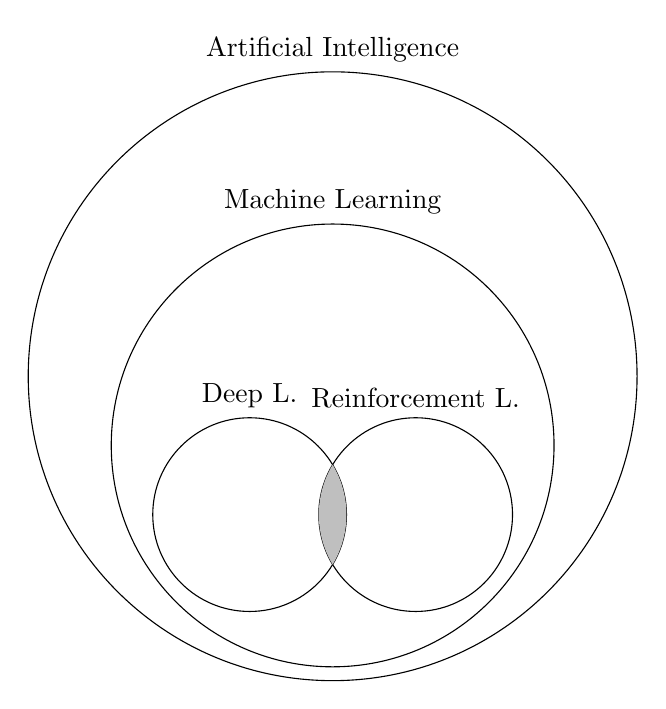
\begin{tikzpicture}

    % Circle with label
    \node[draw,
        circle,
        minimum size =22em,
        label=Artificial Intelligence] (ai_circ) at (0,0){};

    % Circle with label
    \node[draw,
        circle,
        minimum size =16em,
        label=Machine Learning] (ml_circ) at (0,-2.5em){};

    % Circle with label
    \node[draw,
        circle,
        minimum size =7em,
        label=Deep L.] (dl_circ) at (-3em,-5em){};

    \node[draw,
        circle,
        minimum size =7em,
        label=Reinforcement L.] (rl_circ) at (3em,-5em){};


    % Intersection
    \begin{scope}
        \clip (-3em,-5em) circle(3.5em);
        \clip (3em,-5em) circle(3.5em);
        \fill[gray!50](3em,-5em) circle(3.5em);
    \end{scope}

\end{tikzpicture}
    \captionsetup{format=hang} % hanging captions
    \caption{
        The relationship between the fields of Artificial Intelligence,
        Machine Learning, Deep Learning and Reinforcement Learning with some
        arbitrary example provided per field.
    }
    \label{fig:al-ml-dl}
\end{figure}

\section{Machine Learning Fundamentals}
%%%%%%%%%%%%%%%%%%%%%%%%%%%%%%%%%%%%%%%%%%%%%%%%%%%%%%%%%%%%%%%%%%%%%%%%%%%%%%%%
This section aims at providing a non-exhaustive coverage of the basics of
\gls{ML} which can be applied to all \gls{ML} algorithms. This section starts by
defining what is meant when it is said that an algorithm ``learns". The types of
datasets that may be encountered in the application of these learning algorithms
are then briefly covered to provide insight into the potential applications
which are not covered in this review. This is then followed by making the
distinction between the goal of fitting training data and the goal of finding
patterns that generalize to new data. Finally, a very common concept in machine
learning is covered: \textit{hyperparameters}, which are \textit{settings} of a
learning algorithm which must be determined outside the learning algorithm
itself.

\subsection{Learning algorithms\label{ssec:learning_algo}}
%%%%%%%%%%%%%%%%%%%%%%%%%%%%%%%%%%%%%%%%%%%%%%%%%%%%%%%%%%%%%%%%%%%%%%%%%%%%%%%%
Generally speaking, a machine learning algorithm is a procedure for learning
from data. However correct this definition is, it provides little insight into
the relevant concepts in the field. A more succint definition is provided by
Mitchell~\cite{Mitchell97LearningAlgorithm}:

\begin{fancyquotes}
    A computer program is said to learn from experience $E$ with respect
    to some class of tasks $T$ and a performance measure $P$, if its performance
    at tasks in $T$, as measured by $P$, improves with experience $E$.
\end{fancyquotes}

This definition introduces the general entities which are present during all
machine learning tasks. The entities will not be formally defined in the
following sections as it is far outside the scope of this literature, and is
philosophical in nature. This section will instead cover examples of each which
will provide practical insight on which the reader can build their knowledge.

\subsubsection{The Task, $T$}
%%%%%%%%%%%%%%%%%%%%%%%%%%%%%%%%%%%%%%%%%%%%%%%%%%%%%%%%%%%%%%%%%%%%%%%%%%%%%%%%
There exists a plethora of tasks which humanity has applied learning algorithms
to during the timeline of the field. It is common for \gls{ML} practitioners to
originate from domains outside that of computer science, in order to assess the
feasibility of existing algorithms in their domain. There is however a question
that often presents itself to specialists in their respective fields when they
consider applying \gls{ML} to the existing problems in their field. Why should a
specialist opt for solving problems with \gls{ML} that have been solved using
tried and true techniques in their domain of expertise? Goodfellow et al.
\cite{Goodfellow-et-al-2016} provides an insightful response to this:

\begin{fancyquotes}
    Machine learning enables us to tackle tasks that are too difficult
    to solve with fixed programs written and designed by human beings. From a
    scientific and philosophical point of view, machine learning is interesting
    because developing our understanding of it entails developing our
    understanding of the principles that underlie intelligence.
\end{fancyquotes}

An example of a field which has undergone dramatic changes in a short period of
time, with the advent of \gls{DL} and modern hardware, is \gls{CV}. Mahony et
al. discuss this in their paper with a focus on comparing \gls{DL} and \gls{CV}
\cite{Mahony-et-al-2020}. Their paper concludes that many \gls{CV} techniques
invented in the 20 years preceding the paper have become irrelevant as a result
of \gls{DL}. However, they emphasise on the importance of the knowledge
established in those 20 years, arguing that \textit{``knowledge is never
obsolete"}, as it provides specialists with more tools and intuition when
addressing problems. Some typical applications of \gls{CV} are detailed and
although these may be outperformed by \gls{DL}, relying on \gls{DL} in some
cases is overkill. They also point out some hybrid approaches between \gls{DL}
and \gls{CV} which synergize, saying that \gls{CV} provides improved performance
in \gls{DL} by reducing training time. This emphasises that specialists should
not expect an end-all solution from \gls{ML} in addressing their domain-specific
problems, but rather as mentioned by Goodfellow et al., strive for a better
understanding of the principles that underlie intelligence, and by extension,
those that underlie the practitioners domain-specific problems.

\begin{itemize}
    \item \textbf{Classification}: In this task, the learning algorithm is
    expected to produce a function $f: \mathbb{R^n}\rightarrow
    \{1,...,k\}$. When $y=f(\mathbf{x})$, the model assigns a provided
    input, $\mathbf{x}$ to a category identified by numeric code $y$. An
    example of this would be the mapping of a grayscale image,
    $\mathbf{x}\in\mathbb{R}^2$ to a value corresponding to a numerical
    encoding $f:\mathbb{R}^n\rightarrow\{\textrm{Cat},\;\textrm{Dog}\}$.
    \item \textbf{Classification with missing inputs}: Classification becomes
    more challenging when the input measurements to the model are not
    guaranteed to always be the same. In this situation the algorithm must
    learn the set of all function mappings arising from the possible
    combinations of input vectors that arise from missing subsets of
    inputs in $\mathbf{x}$. An example of this would be the classification
    of a diagnosis in medicine, as depending on the invasiveness of
    certain procedures, different subsets of measurements are available.
    \item \textbf{Regression}: In this task, the learning algorithm is expected
    to predict a continuous numerical value for a given input. This is
    done by learning a function $f: \mathbb{R}^n\rightarrow\mathbb{R}$.
    the formulation is similar to that of classification, except for the
    output format. An example of this would be learning of a function to
    predict the expected returns for a given investment given the state of
    the market, as is common is algorithmic trading.
    \item \textbf{Transcription}: This type of task involves the learning
    algorithm observing a relatively unstructured input and transcribing
    it into some discrete textual form. An example of this is the
    transcription of an audio waveform containing speech into text.
    \item \textbf{Machine translation}: In machine translation, the already
    structured input is mapped into a different language. This is common
    in the field of \gls{NLP}, where languages are translated between, for
    example English and French. This however is not limited to natural
    languages but can also be applied to programming languages for
    example.
    \item \textbf{Structured output}: This task entails those where the output
    is a vector or a data structure which details important relationships
    between the contained elements. This task subsumes the prior two of
    transcription and machine translation. An example of this would be the
    parsing of grammatical structure of a natural language sentence,
    addressed in \gls{NLP} and demonstrated by Collobert
    \cite{pmlr-v15-collobert11a}.
    \item \textbf{Anomaly detection}: In this task, a learning algorithm learns
    to sift through a set of events and classify events that are anomalous
    in nature. These algorithms have been applied to credit card companies
    in detection of fraud \cite{DBLP:journals/corr/abs-2108-10005}, and in
    safety in the aviation industry \cite{Janakiraman2016, Basora2019}.
    \item \textbf{Synthesis and sampling}: In this task, learning algorithms
    generate \textbf{new} examples which appear to be drawn from the same
    underlying distribution as, but are not present in the training data.
    A recent example around which a lot of research is being done is the
    \gls{GPT-3} which is able to produce human-like text, given prompts as
    input \cite{DBLP:journals/corr/abs-2005-14165}.
    \item \textbf{Imputation of missing values}: In this task, the learning
    algorithm is given some input $x\in\mathbb{R}$ with some elements
    $x_i$ missing. The algorithm must then make predictions for the
    missing values. Emmanuel et al. discuss the latest methods in
    \gls{ML} that address this task~\cite{Emmanuel2021}. A recent example of
    imputation of missing frames for the purpose of adding frames to videos
    is \gls{RIFE} \cite{huang2020rife}.
    \item \textbf{Denoising}: In this learning task, the machine learning
    algorithm learns to generate a clean example $\mathbf{x}\in\mathbb{R}^n$
    from a corrupted sample $\tilde{\mathbf{x}}\in\mathbb{R}^n$. Generally
    speaking the learner is predicting the probability distribution
    $p(\mathbf{x}|\tilde{\mathbf{x}})$.
    \item \textbf{Density estimation} or \textbf{probability mass function estimation}
    involves the task of learning a function $p_\text{model}:\mathbb{R}^n\rightarrow{}\mathbb{R}$,
    where $p_\text{model}(\mathbf{x})$ is interpreted as a probability distribution function
    from which $\mathbf{x}$ was drawn. Effectively the algorithm learns the
    structure of the data that it has been provided with. Most of the
    aforementioned tasks involve learning this distribution function, at least
    implicitly. For example for the missing value imputation task, if $x_i$ is
    missing, and all other values $x_{-i}$ are given, then the algorithm learns
    the distribution $p(x_i|\mathbf{x}_{-i})$ which involves $p(\mathbf{x})$
    implicitly.
\end{itemize}
%An ongoing trend in society is the augmentation of responsibility in intelligent
%algorithms through autonomy, evident by the advent of semi-autonomous cars,
%autonomous cyber-security \cite{Taeihagh2019}, autonomous industrial site
%inspection\footnote{\url{https://newsroom.ibm.com/Boston-Dynamics-and-IBM-Join-Forces-to-Bring-Mobile-Edge-Analytics-to-Industrial-Operations}},
%and autonomous supply-chain
%management\footnote{\url{https://www.forbes.com/sites/stevebanker/2021/04/01/amazon-supply-chain-innovation-continues/}},
%to name a few.

%This section reviews the current ongoing research in the field of machine
%learning as a whole. First the main categories:

\subsubsection{The Performance, $P$\label{sec:ML-performance}}
%%%%%%%%%%%%%%%%%%%%%%%%%%%%%%%%%%%%%%%%%%%%%%%%%%%%%%%%%%%%%%%%%%%%%%%%%%%%%%%%
In order to assess the performance of our learning algorithm in task $T$,
we must have some quantitative measure of performance $P$ with which we steer
the algorithm towards the desired behaviour. $T$ and $P$ in this way are
coupled, and must $P$ must be chosen according to $T$. In this way it can be
unclear to the \gls{ML} practitioner what $P$ should be chosen.

Firstly, it is worth considering the true goal of the learning algorithm. We
wish for it to train according to some dataset such that it can generalize to
inputs that it has never seen before. After all, there is little worth in a
classification algorithm recognizing cats and dogs with 90\% accuracy on its
training dataset, if it performs with 20\% accuracy on an unseen \textbf{test}
dataset. This previously mentioned scenario is known as \textit{overfitting} and
is discussed in its own section later in the chapter. For this reason, the first
requirement on managing our dataset is presented, there must be some
\textbf{train-test split}. This is further complicated by the
\textbf{validation} dataset which is discussed later in the chapter.

Given that the input-output pair is $\{\gls{x_in_i}, \gls{y_true_i}\}$,
\gls{y_true_i} is commonly referred to as the \textit{ground truth}, and
$\hat{\mathbf{f}}(\gls{x_in_i})=\gls{y_pred_i}$ are referred to as the
\textit{predictor} and \textit{predicted output} respectively. The performance
in the form of a loss function \gls{J} (also referred to as an objective or cost
function in literature) is then a function of \gls{y_true_i} and
\gls{y_pred_i}, therefore $\gls{J}(\gls{y_pred_i}, \gls{y_true_i})$.

\gls{ML} often borrows from \textit{approximation theory} vector norm notation
($\ell(\cdot)_p=||\cdot||_p$) to simplify notation in performance metrics. See
\autoref{appendix:vector_norms} for the expressions of vector norms.

\textbf{Regression loss functions}
\begin{itemize}
    \item \textbf{\Gls{MSE}} is the average of the squared differences between
    predictions and the ground truth. It is only concerned with the average
    magnitude of errors irrespective of their direction. Due to the squaring,
    predictions which have greater errors are more heavily penalized. A
    beneficial mathematical property of \gls{MSE} is that gradients can be
    easily calculated.
    \begin{equation}
        \gls{J}_\text{\gls{MSE}} = \frac{1}{\gls{ml:m}}\sum_{i=1}^{\gls{ml:m}}||\gls{y_pred_i}-\gls{y_true_i}||^2_2
        \label{eq:MSE}
    \end{equation}
    \begin{equation*}
        \begin{aligned}
            \textrm{where, }
            \eqdesc{J}\text{,} \\
            \eqdesc{m}\text{,} \\
            \eqdesc{y_pred_i}\text{,} \\
            \eqdesc{y_true_i}\text{.} \\
        \end{aligned}
    \end{equation*}
    \item \textbf{L2 error} is the average of the differences between
    predictions and the ground truth. It is the same as \gls{MSE} but without
    the squaring. Like \gls{MSE}, the gradient can be easily calculated.
    \begin{equation}
        \gls{J}_\text{L2E} = \frac{1}{\gls{ml:m}}\sum_{i=1}^{\gls{ml:m}}||\gls{y_pred_i}-\gls{y_true_i}||_2
    \end{equation}
    \item \textbf{\Gls{MAE}} or \textbf{L1 loss} is the average of the sum of
    absolute differences between predictions and the ground truth. This measure
    is similar to \gls{MSE} in that it considers the magnitude of the errors and
    ignores their direction. However, \gls{MAE} is more difficult to compute
    gradients for, requiring linear programming. \gls{MAE} is also more
    resilient to large error values as a result of outliers, as it does not make
    use of a square.
    \begin{equation}
        \gls{J}_\text{MAE} = \frac{1}{\gls{ml:m}}\sum_{i=1}^{\gls{ml:m}}||\gls{y_pred_i}-\gls{y_true_i}||_1
        \label{eq:MAE}
    \end{equation}
    \item \textbf{\Gls{MBE}} is the sum of all differences between predictions
    and the ground truth. \gls{MBE} is not often used as a measure of the model
    error as high individual errors can produce a low \gls{MBE}. This metric is
    primarily used to measure the average bias of a prediction.
    \begin{equation}
        \gls{J}_\text{MBE} = \frac{1}{\gls{ml:m}}\sum_{i=1}^{\gls{ml:m}}\sum_{j=1}^{\gls{ml:n_y}}(\gls{y_pred_ij}-\gls{y_true_ij})
    \end{equation}
    \begin{equation*}
        \begin{aligned}
            \textrm{where, }
            \eqdesc{n_y}\text{,} \\
            \eqdesc{y_pred_ij}\text{,} \\
            \eqdesc{y_true_ij}\text{.} \\
        \end{aligned}
    \end{equation*}
    \item \textbf{\Gls{MSLE}} can be interpreted as a measure of the ratio
    between predictions and the ground truth. This metric is used when it is
    desirable to achieve some relative measure of accuracy as opposed to an
    absolute. In other words, large and small discrepancies between the
    predicted and ground truth are dealt in a relative manner, resulting in
    similar loss value magnitudes.
    \begin{equation}
        \begin{aligned}
            \gls{J}_\text{MSLE} &= \frac{1}{\gls{ml:m}}\sum_{i=1}^{\gls{ml:m}}\sum_{j=1}^{\gls{ml:n_y}}(\log{(\gls{y_true_ij}+1)} - \log{(\gls{y_pred_ij}+1)})^2 \\
            &= \frac{1}{\gls{ml:m}}\sum_{i=1}^{\gls{ml:m}}\sum_{j=1}^{\gls{ml:n_y}}2\log(\frac{\gls{y_true_ij}+1}{\gls{y_pred_ij}+1})
        \end{aligned}
    \end{equation}
    \item \textbf{\Gls{CP}} or \textbf{\gls{CS}} is a measure of similarity
    between two non-zero vectors of an inner product space. The metric is
    defined as the cosine of the angle between the two vectors. The metric is
    bounded in the interval $[-1,1]$, -1 for opposing orientation and 1 for the
    same orientation. This is not often useful in some \gls{ML} tasks, so an
    alternative form known as the \textbf{\gls{CD}} is used instead. The
    relation between the metrics is $\text{\gls{CD}}=1-\text{\gls{CP}}$,
    bounding the error in the interval $[0,2]$.
    \begin{equation}
        \gls{J}_\text{\gls{CD}} =
        \frac{1}{\gls{ml:m}}\sum_{i=1}^{\gls{ml:m}}\bigg(1-\frac{\gls{y_true_i}\cdot{}\gls{y_pred_i}}{||\gls{y_true_i}||_2\cdot{}||\gls{y_pred_i}||_2}\bigg)
    \end{equation}
\end{itemize}

\textbf{Binary classification loss functions}\\
Binary classification differs from multi-class in that the output is a single
value (\gls{ml:n_y}$=1$). For multi-class, the dimension of the output is equal to
the number of classes.

\begin{itemize}
    \item \textbf{\Gls{BCE}}, also known as \textbf{maximum likelihood}, is a
    measure defined simply by the negative log-likelihood between the training
    data and model distribution. In the case where $\gls{y_true_i1}=1$ and
    $\gls{y_pred_i1}=0$, the log probability of the predicted output is
    undefined. For this reason, practitioners often add some small constant on
    the probability of \gls{y_pred_i1}, e.g. $10^{-5}$, resulting in
    \gls{J}$\approx{}5$.
    \begin{equation}
        \gls{J}_\text{\gls{BCE}}=-\sum_{i=1}^{\gls{ml:m}}\bigg(\gls{y_true_i1}\log(\gls{y_pred_i1})+(1-\gls{y_true_i1})\log(1-\gls{y_pred_i1})\bigg)\label{eq:equation}
    \end{equation}
    \item \textbf{\Gls{HL}} is measure which is often used for training binary
    \gls{SVM} classifiers. The loss function assumes that \gls{y_true_ij} and
    \gls{y_pred_ij} are in the bounds $[-1,1]$ for the classification task.
    \begin{equation}
        \gls{J}_\text{\gls{HL}}=\sum_{i=1}^{\gls{ml:m}}\max(0, {1-\gls{y_true_i1}\cdot{}\gls{y_pred_i1}})
    \end{equation}
    \item \textbf{\Gls{SHL}} addresses the constant gradient present in
    \gls{HL}, smoothing the loss function across the domain of the loss function
    ($\gls{y_true_ij}\cdot{}\gls{y_pred_ij}$). This provides better gradient
    learning properties, as predictions that are more incorrect than others have
    a heavier associated gradient.
    \begin{equation}
        \gls{J}_\text{\gls{SHL}}=\sum_{i=1}^{\gls{ml:m}}\max(0, {1-\gls{y_true_i1}\cdot{}\gls{y_pred_i1}})^2
    \end{equation}
\end{itemize}

\textbf{Multi-class classification loss functions}
Multi-class classification is formulated such that each possible class ($n_c$)
is defined by an element of the output vector. The loss functions here are
similar to the binary classification loss functions, but adapted for
$\gls{ml:n_y}=n_c$.

\begin{itemize}
    \item \textbf{\Gls{MCE}}:
    \begin{equation}
        \gls{J}_\text{\gls{MCE}}=-\sum_{i=1}^{\gls{ml:m}}\sum_{j=1}^{\gls{ml:n_y}}\gls{y_true_ij}\log(\gls{y_pred_ij})
    \end{equation}
    \item \textbf{\Gls{MHL}}:
    \begin{equation}
        \gls{J}_\text{\gls{MHL}}=\sum_{i=1}^{\gls{ml:m}}\sum_{j=1}^{\gls{ml:n_y}}\max(0, {1-\gls{y_true_ij}\cdot{}\gls{y_pred_ij}})
    \end{equation}
    \item \textbf{\Gls{MSHL}}:
    \begin{equation}
        \gls{J}_\text{\gls{MSHL}}=\sum_{i=1}^{\gls{ml:m}}\sum_{j=1}^{\gls{ml:n_y}}\max(0, {1-\gls{y_true_ij}\cdot{}\gls{y_pred_ij}})^2
    \end{equation}
\end{itemize}


\begin{itemize}
\end{itemize}

%With the
%In the case of classification, most metrics are derived from the confusion
%matric

\subsubsection{The Experience, $E$\label{sec:ML-experience}}
%%%%%%%%%%%%%%%%%%%%%%%%%%%%%%%%%%%%%%%%%%%%%%%%%%%%%%%%%%%%%%%%%%%%%%%%%%%%%%%%
Tasks provided to machine learning algorithms have different formulations based
on the experience made available. Learning algorithms can be broadly categorized
by the kind of experience that the algorithm has access to during learning, from
which it is generally expected to learn some pattern of interest.

\begin{itemize}
    \item \textbf{Supervised learning} algorithms experience a dataset
    containing features (input) and labels (expected output), and are expected
    to learn a function mapping between the two. These algorithms can be further
    divided into two categories. \textbf{Classification algorithms} learn a
    mapping from an input to a discrete class label output. \textbf{Regression
    algorithms} learn a mapping from an input to a continuous value output.

%    example input-output pairs, otherwise referred to as the labelled training
%    data consisting of a set of training examples. The trained \textit{model} is
%    then provided an unseen $x$ for which it must estimate $y$ based on its
%    experience. Supervised models are further grouped into two subcategories,
%    classification and regression. \textbf{Classification} is the task of
%    mapping $x$ to a discrete output variable $y$ which determines the predicted
%    class based on the $x$. A simple example of this would be a $y$ in
%    $\mathbb{R}^2$ which determines whether the input image was a \textit{cat}
%    or a \textit{dog}. \textbf{Regression} is task of mapping $x$ onto a
%    continuous output variable $y$ which determines the value of some variable
%    of interest. An example of this would be the task of learning an
%    approximator to the function: $f(x)=x^2$.
    % Dimensionality reduction \cite{vogelstein2021supervised}

    \item \textbf{Unsupervised learning} algorithms experience a dataset
    containing only features and learn some useful properties of the structure
    of the dataset. This form of learning often addresses recognition problems
    in \textit{association} \& \textit{clustering} \cite{barlow1999ul}.

    \item \textbf{Semi-supervised} is a middle ground between supervised
    learning (in which all training data is labelled) and unsupervised learning
    (in which no label data is provided)~\cite{books/mit/06/CSZ2006}. Some
    example applications of this paradigm are dimensionality reduction
    ~\cite{Zhang2007}, clustering \cite{Bair2013}, and anomaly detection
    \cite{DBLP:journals/corr/abs-1805-06725}.

    \item \textbf{Reinforcement learning} are learning algorithms which rely
    exclusively on a series of reinforcements from its environment. These
    reinforcements can be positive (rewards) or negative (punishments). This
    category is discussed further in \autoref{ssec:RL}.
\end{itemize}

\subsection{Capacity, Overfitting and Underfitting\label{sec:capoverunder}}
%%%%%%%%%%%%%%%%%%%%%%%%%%%%%%%%%%%%%%%%%%%%%%%%%%%%%%%%%%%%%%%%%%%%%%%%%%%%%%%%
The primary objective in \gls{ML} is to find a model which performs well on
previously \textit{unseen data}, which has not been used during the training or
fitting of a model. This ability of the learning algorithm is referred to as its
ability to \textit{generalise}.

Typically the learning algorithm is trained according to a set of
\textit{training data} with which we aim at reducing the learners
\textbf{training error}. Due to this data having been directly used to optimise
the model during training, we cannot expect this error to be representative of
the model's \textbf{generalisation error}. In order to derive an estimate of the
generalisation error, we separate part of the initial data set into training and
\textbf{test data}, from which the \textbf{test error} is derived. Given some
assumptions about the \textbf{data-generating process}, such as the data being
\textbf{\gls{iid}}, it can be said that the training error is equal to the
expectation of the test error.

An important concept in \gls{ML} is the \textit{capacity} of the model. This is
defined informally as \textit{``a model’s [...] ability to fit a wide
variety of functions"}~\cite[p.~111-112]{Goodfellow-et-al-2016}. Machine learning
algorithms will generally perform their best when their capacity is appropriate
for the true complexity of the task they are expected to perform given the
available training data. Models with insufficient capacity will fail to perform
complex tasks and those with excessive capacity will perform complex tasks, but
they may overfit the training data.

One technique of controlling the capacity of an algorithm is to control its
\textbf{hypothesis space}, the set of possible functions that the algorithm may
use to solve the task at hand. In the case of a polynomial, such as the
arbitrary one seen in \autoref{fig:capacity-plots}, this effect can be
intuitively related to the models propensity to underfit and overfit a set of
training data.

\begin{figure}[htp]
    \centering
    % MIT License
%
% Copyright (c) 2021 Geoffrey H. Garrett
%
% Permission is hereby granted, free of charge, to any person obtaining a copy
% of this software and associated documentation files (the "Software"), to deal
% in the Software without restriction, including without limitation the rights
% to use, copy, modify, merge, publish, distribute, sublicense, and/or sell
% copies of the Software, and to permit persons to whom the Software is
% furnished to do so, subject to the following conditions:
%
% The above copyright notice and this permission notice shall be included in all
% copies or substantial portions of the Software.
%
% THE SOFTWARE IS PROVIDED "AS IS", WITHOUT WARRANTY OF ANY KIND, EXPRESS OR
% IMPLIED, INCLUDING BUT NOT LIMITED TO THE WARRANTIES OF MERCHANTABILITY,
% FITNESS FOR A PARTICULAR PURPOSE AND NONINFRINGEMENT. IN NO EVENT SHALL THE
% AUTHORS OR COPYRIGHT HOLDERS BE LIABLE FOR ANY CLAIM, DAMAGES OR OTHER
% LIABILITY, WHETHER IN AN ACTION OF CONTRACT, TORT OR OTHERWISE, ARISING FROM,
% OUT OF OR IN CONNECTION WITH THE SOFTWARE OR THE USE OR OTHER DEALINGS IN THE
% SOFTWARE.

%%%%%%%%%%%%%%%%%%%%%%%%%%%%%%%%%%%%%%%%%%%%%%%%%%%%%%%%%%%%%%%%%%%%%%%%%%%%%%%
% ACKNOWLEDGEMENTS
%%%%%%%%%%%%%%%%%%%%%%%%%%%%%%%%%%%%%%%%%%%%%%%%%%%%%%%%%%%%%%%%%%%%%%%%%%%%%%%
% Design and implementation of this diagram was inspired and adapted from:
% https://tex.stackexchange.com/questions/573127/tikz-plots-are-not-centered

%%%%%%%%%%%%%%%%%%%%%%%%%%%%%%%%%%%%%%%%%%%%%%%%%%%%%%%%%%%%%%%%%%%%%%%%%%%%%%%
% DEPENDENCIES
%%%%%%%%%%%%%%%%%%%%%%%%%%%%%%%%%%%%%%%%%%%%%%%%%%%%%%%%%%%%%%%%%%%%%%%%%%%%%%%
%\usepackage{tikz}
% \usetikzlibrary{positioning, decorations.text, calc}

%%%%%%%%%%%%%%%%%%%%%%%%%%%%%%%%%%%%%%%%%%%%%%%%%%%%%%%%%%%%%%%%%%%%%%%%%%%%%%%
% USER STYLING
%%%%%%%%%%%%%%%%%%%%%%%%%%%%%%%%%%%%%%%%%%%%%%%%%%%%%%%%%%%%%%%%%%%%%%%%%%%%%%%


%

%\tikzset{declare function={f(\x)=(-0.06*(\x-2)+0.5)*(\x-2)*(\x-2);}}% applied math style
%\foreach \Z in {1,...,42} {\pgfmathsetmacro{\X}{\Z/10}%
%\pgfmathsetmacro{\Y}{f(\X)+0.9*rnd}%
%\ifnum\Z=1
%\xdef\LstOne{(\X,\Y)}%
%\xdef\LstTwo{"(\X,\Y)"}%
%\else
%\xdef\LstOne{\LstOne (\X,\Y)}%
%\xdef\LstTwo{\LstTwo,"(\X,\Y)"}%
%\fi}%

\newcommand{\plotobservations} {
    \addplot[only marks, draw=blue, fill=blue] coordinates {
        (0.0, 2.5991314214589614)
        (0.4444444444444444, 1.3463852235976501)
        (0.8888888888888888, 1.3558966978583558)
        (1.3333333333333333, 0.1719351250071693)
        (1.7777777777777777, 0.0549444514647925)
        (2.2222222222222223, 0.45130282341732175)
        (2.6666666666666665, -0.04104830486674099)
        (3.1111111111111107, 0.3752375262271346)
        (3.5555555555555554, 1.034685792786699)
        (4.0, 1.430935111399573)
    };
}

\newcommand{\plottruedistribution}{
    \addplot[domain=-0.5:4.5, dashed, thin, gray!75] {
        (-0.06 * (x - 2) + 0.5) * (x - 2) * (x - 2)
    };


}

%%%%%%%%%%%%%%%%%%%%%%%%%%%%%%%%%%%%%%%%%%%%%%%%%%%%%%%%%%%%%%%%%%%%%%%%%%%%%%%%
\begin{subfigure}[b]{0.32\textwidth}
    \centering
    \begin{tikzpicture}
        \begin{axis}[
            xmin=-0.5,
            xmax=4.5,
            ymin=-0.5,
            ymax=3.5,
            ticks=none,
            xticklabels={\empty},
            yticklabels={\empty},
            ymajorgrids=false,
            xmajorgrids=false,
            axis line style = semithick,
            width=1.2\columnwidth]
            \plotobservations
            \plottruedistribution
            \addplot[domain=-0.5:4.5, thick, green!50!black] {
                1.3645283299815407 - 0.24329387 * x
            };
        \end{axis}
    \end{tikzpicture}
    \subcaption{Underfitting}
    \label{fig:underfitting}
\end{subfigure}\hfil
%%%%%%%%%%%%%%%%%%%%%%%%%%%%%%%%%%%%%%%%%%%%%%%%%%%%%%%%%%%%%%%%%%%%%%%%%%%
\begin{subfigure}[b]{0.32\textwidth}
    \centering
    \begin{tikzpicture}
        \begin{axis}[
            xmin=-0.5,
            xmax=4.5,
            ymin=-0.5,
            ymax=3.5,
            ticks=none,
            xticklabels={\empty},
            yticklabels={\empty},
            ymajorgrids=false,
            xmajorgrids=false,
            axis line style = semithick,
            width=1.2\columnwidth]
            \plotobservations
            \plottruedistribution
            \addplot[domain=-0.5:4.5, thick, green!50!black] {
                + 2.5332784046893866
                - 2.31697944 * x
                + 0.58870681 * x ^ 2
                - 0.01887639 * x ^ 3
            };
        \end{axis}
    \end{tikzpicture}
    \subcaption{Appropriate capacity}
    \label{fig:appropriate-capacity}
\end{subfigure}\hfil
%%%%%%%%%%%%%%%%%%%%%%%%%%%%%%%%%%%%%%%%%%%%%%%%%%%%%%%%%%%%%%%%%%%%%%%%%%%%%%%%%%%
\begin{subfigure}[b]{0.32\textwidth}
    \centering
    \begin{tikzpicture}
        \begin{axis}[
            xmin=-0.5,
            xmax=4.5,
            ymin=-0.5,
            ymax=3.5,
            ticks=none,
            xticklabels={\empty},
            yticklabels={\empty},
            ymajorgrids=false,
            xmajorgrids=false,
            samples=200,
            axis line style = semithick,
            width=1.2\columnwidth]
            \plotobservations
            \plottruedistribution
            \addplot[domain=-0.5:4.5, thick, green!50!black] {
                +2.599131312448361
                -10.588139742958015 * x^1
                +25.074367329152583 * x^2
                -12.832852119149837 * x^3
                -15.29078616509039 * x^4
                +10.350960340047243 * x^5
                +10.94777207200677 * x^6
                -14.543216443491573 * x^7
                +6.786937457668481 * x^8
                -1.5968672908165933 * x^9
                +0.18962693236609746 * x^10
                -0.009014002246939552 * x^11
            };
        \end{axis}
    \end{tikzpicture}
    \subcaption{Overfitting}
    \label{fig:overfitting}
\end{subfigure}

    \captionsetup{format=hang} % hanging captions
    \caption{
        Three different models fit to an arbitrary example training set
        generated from an arbitrary third-degree polynomial (dashed line) with
        some added noise. (a) Shows that first-degree polynomial (linear model)
        fails in generalising well to the data, and results in
        \textbf{underfitting}. (b) Shows a third-degree polynomial generalising
        well and is described as having an \textbf{appropriate capacity},
        potentially optimal. (c) Shows an eleventh-degree polynomial which has a
        high variance in error and is described as \textbf{overfitting}.
    }
    \label{fig:capacity-plots}
\end{figure}

\begin{figure}[htp]
    \centering
    % Adapted from https://raw.githubusercontent.com/MartinThoma/LaTeX-examples/master/tikz/bias-variance/bias-variance.tex

%\usetikzlibrary{arrows.meta,bending}
\tikzset{>=stealth,
    OptimumStyle/.style={align=center,anchor=center,rotate=90,font=\sffamily\scriptsize},
    OverfitStyle/.style={align=center,anchor=west,rotate=0,font=\sffamily\scriptsize},
    UnderfitStyle/.style={align=center,anchor=east,rotate=0,font=\sffamily\scriptsize},
}
\pgfplotsset{compat=1.17,
    samples=101,
    axis lines = left,
    every axis plot/.append style={line width=2pt},
}

%\begin{document}
%\fbox{
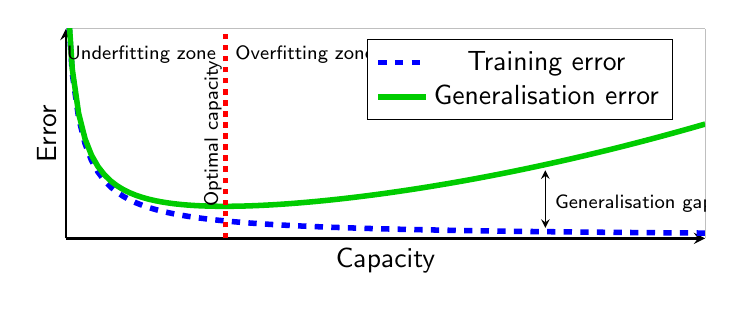
\begin{tikzpicture}[font=\sffamily\sansmath]

    \begin{axis}
        [
        xmin=0,
        xmax=2,
        ymin=0,
        ymax=2,
        xlabel=Capacity,
        ylabel=Error,
        ticks=none,
        xtick={2},
        ytick={2},
        xticklabels={\empty},
        yticklabels={\empty},
        ymajorgrids=true,
        xmajorgrids=true,
        width=0.8\linewidth,
        height=0.35\linewidth,
        axis line style = thick,
        legend style={at={(0.95,0.95)},anchor=north east}
        ]
        \addplot[domain=0.00:2.0, blue, dashed] {0.25/(3*x+0.1) + 0.01};   % Training error
        \addlegendentry{Training error}
        \addplot[domain=0.00:2.0, green!80!black] {0.25/(3*x+0.1) + 0.1*x + 0.2 *x*x + 0.05};  % Generalisation error
        \addlegendentry{Generalisation error}
%      \addplot[domain=0.39:1.61,black] {3*(x-2)*x+3.8};  %Total error
        \addplot[dotted, red] coordinates {(0.5,0) (0.5,2)};           %Optimum model complexity
        \addplot[thin, <->] coordinates {(1.5,0.1) (1.5,0.65)};       %Optimum model complexity

        \node[OptimumStyle] at (axis cs:0.46,1.0) {Optimal capacity};
        \node[UnderfitStyle] at (axis cs:0.5,1.75) {Underfitting zone};
        \node[OverfitStyle] at (axis cs:0.5,1.75) {Overfitting zone};
        \node[OverfitStyle] at (axis cs:1.5,0.33) {Generalisation gap};
%      \node[anchor=south west,text=Maroon] at (axis cs:1.4,0.4){Bias\textsuperscript{2}};
%      \node[anchor=north west,text=TealBlue] at (axis cs:1.4,0.85){Variance};
%      \node[anchor=south east,align=center] at (axis cs:1.5,1.5){Total\\error};
%        \legend{}
    \end{axis}
\end{tikzpicture}
%}

%\end{document}
    \captionsetup{format=hang} % hanging captions
    \caption{
        Typical relationship between capacity and error. Training and test error
        behave differently. At the left end of the graph, training error and
        generalization error are both high. This is the \textbf{underfitting
        regime} As we increase capacity, training error decreases, but the gap
        between training and generalisation error increases. Eventually, the
        size of this gap outweighs the decrease in training error, and we enter
        the \textbf{overfitting regime}, where capacity is too large, above the
        \textbf{optimal capacity}. Adapted from Goodfellow et al.
        \cite{Goodfellow-et-al-2016}.
    }
    \label{fig:capacity}
\end{figure}

\subsubsection{No Free Lunch Theorem}
%%%%%%%%%%%%%%%%%%%%%%%%%%%%%%%%%%%%%%%%%%%%%%%%%%%%%%%%%%%%%%%%%%%%%%%%%%%%%%%%

The \gls{NFLT}, sometimes abbreviated as \gls{NFL}, is a simple but important
concept in \gls{ML} and optimisation~\cite{Wolpert1997}. The theorem suggests
that an optimisation technique will perform equally well as any other, when
averaging its performance over the set of all possible problems. This implies
that there is no single best technique for addressing an arbitrary problem. Luke
states the following in \textit{essentials of
metaheuristics}~\cite{luke2012essentials}:

\begin{fancyquotes}
    The \gls{NFL} stated that within certain constraints, over the space of
    all possible problems, every optimization technique will perform as well as
    every other one on average (including Random Search)
\end{fancyquotes}

This argues that without having substantive information about the fundamentals
of the problem being modelled, choosing to apply a single technique to an
arbitrary problem will not yield a predictably better or worse result than
applying another to the same problem. Therefore, in the case where the
underlying process being optimised is not well-understood, a variety of
techniques should be applied.

However, in practice, knowledge to some degree is known about the problem which
is being optimised, or to which a learning algorithm is being applied. This
theorem highlights the importance of having a clear understanding of the problem
at hand before applying a learning algorithm or an optimisation technique.
Domingos states ~\cite{Domingos15}:

\begin{fancyquotes}
    In the meantime, the practical consequence of the “no free lunch”
    theorem is that there’s no such thing as learning without knowledge. Data
    alone is not enough.
\end{fancyquotes}

This theorem, in effect, motivates the true goal of machine learning, as worded
by Goodfellow et al.~\cite[p.~116]{Goodfellow-et-al-2016}:

\begin{fancyquotes}
    This means that the goal of machine learning research is not to seek
    a universal learning algorithm or the absolute best learning algorithm.
    Instead, our goal is to understand what kinds of distributions are relevant
    to the “real world” that an AI agent experiences, and what kinds of machine
    learning algorithms perform well on data drawn from the kinds of
    data-generating distributions we care about.
\end{fancyquotes}


This is an important insight and directly relates to a learning algorithm's
tendency to overfit or underfit. If we do not have a clear understanding of the
level of complexity of the task we are trying to find a solution to with our
learning algorithm, then we are likely to overfit or underfit. If one assumes
the complexity of the problem to be higher than its true complexity, the learner
will have access to a much larger hypothesis space (capacity) than what is
optimal. On the other hand, if we underestimate the complexity, it is almost
certain that we will design an algorithm with insufficient capacity. This also
extends to the quantity and quality of training data that we are training with.
It is impossible, for example, to model an $n^\text{th}$ order process with anything less
than $n$ training samples without underfitting, and this is without considering
the possibility of measurement noise.

\subsubsection{Regularization}
%%%%%%%%%%%%%%%%%%%%%%%%%%%%%%%%%%%%%%%%%%%%%%%%%%%%%%%%%%%%%%%%%%%%%%%%%%%%%%%%
Generally speaking, regularization is any modification we make to a learning
algorithm that is intended to reduce its generalisation error but not its
training error. Due to the large number of techniques that fit this description
within \gls{ML} and its subfields, it is outside the scope of this paper to
exhaustively cover this concept, however the core idea behind regularization
within \gls{ML} is motivated here through one of its earliest forms.

A fundamental approach to regularization in \gls{ML} originating from
\textit{statistical learning} is the use of \textbf{parameter norm penalties}.
This technique aims at guiding the parameter vectors through the addition of a
penalty term in the objective (cost/loss) function being minimised. This penalty
constrains (regularizes) or shrinks the optimal \gls{w_vec} estimate towards
zero, effectively discouraging a learning algorithm from producing an
excessively complex model, to avoid overfitting. Norm penalty methods can be
generalized as:

\begin{equation}
    \gls{J_reg}(\gls{ml:theta}; \gls{X}, \gls{Y})
    =
    \gls{J}(\gls{ml:theta}; \gls{X}, \gls{Y})_\text{train}
    +
    \gls{ml:w_reg}\gls{o_reg}({\gls{ml:theta}}),
    \label{eq:norm_penalty_reg}
\end{equation}
\begin{equation*}
    \begin{aligned}
        \textrm{where, }
        \eqdesc{J_reg}\text{,} \\
        \eqdesc{ml:theta}\text{,} \\
        \eqdesc{X}\text{,} \\
        \eqdesc{Y}\text{,} \\
        \eqdesc{J}\text{,} \\
        \eqdesc{ml:w_reg}\text{,} \\
        \eqdesc{o_reg}\text{.} \\
    \end{aligned}
\end{equation*}

For learning algorithms which make use of gradient-based learning techniques,
the parameter gradient must be computed. This can be challenging to compute in
cases where the derivative of a cost function is not easily determined, such as
with \gls{MAE} defined by \autoref{eq:MAE}. The expression of the regularized
cost function is given by,

\begin{equation}
    \nabla_{\gls{w_vec}}\gls{J_reg}(\gls{w_vec};\gls{X},\gls{Y})
    =
    \nabla_{\gls{w_vec}}\gls{J}(\gls{w_vec};\gls{X},\gls{Y})
    +
    \gls{ml:w_reg}\nabla_{\gls{w_vec}}\gls{o_reg}(\gls{ml:theta})\text{.}
    \label{eq:norm_penalty_reg_graident}
\end{equation}

$\bm{\text{L}^2}$ \textbf{regularization}, also known as \textbf{ridge
regression}, \textbf{weight decay} or \textbf{Tikhonov regularization}
\cite[p.~227]{Goodfellow-et-al-2016}, is a parameter norm regularization method
which drives the weights of a model towards the origin in the weight space and
contributes to \autoref{eq:norm_penalty_reg} as,
\begin{equation}
    \gls{o_reg}(\gls{ml:theta})=\frac{1}{2}||\gls{w_vec}||^2_2.
    \label{eq:l2_reg}
\end{equation}

Weight decay suppresses any irrelevant components of the weight vector by
choosing the smallest vector that solves the learning problem. Furthermore if
the weight decay parameter is chosen correctly, noise may be suppressed in the
output, subsequently improving generalization~\cite{NIPS1991_8eefcfdf}.

$\bm{\text{L}^1}$ \textbf{regularization}, also known as \textbf{\gls{LASSO}
regression} is a parameter norm regularization method which penalizes the
largest weight magnitudes in the weight vector. It is defined by,
\begin{equation}
    \gls{o_reg}(\gls{ml:theta})=||\gls{w_vec}||_1.
    \label{eq:l1_reg}
\end{equation}

The key difference between $L^1$ and $L^2$ regularization is that $L^1$
regularization tends to better constrain values of $\gls{w_vec}$ to zero,
effectively performing feature selection on the inputs through their weights. It
can be less intuitive to interpret the $L^2$ regularization as a feature
selection method, as it can be unclear whether the weights are truly being
constrained to zero or their importance for generalization is just less than
other elements in \gls{w_vec}. This is seen in
\autoref{fig:l1-l2-regularization}, where the $L^1$ regularization has reduced
$w_1$ to zero, with a negligible impact on the performance, whereas the $L^2$
variant has not.

\begin{figure}[!htp]
    \centering
    \begin{subfigure}[b]{0.49\textwidth}
        \centering
        % MIT License
%
% Copyright (c) 2021 Geoffrey H. Garrett
%
% Permission is hereby granted, free of charge, to any person obtaining a copy
% of this software and associated documentation files (the "Software"), to deal
% in the Software without restriction, including without limitation the rights
% to use, copy, modify, merge, publish, distribute, sublicense, and/or sell
% copies of the Software, and to permit persons to whom the Software is
% furnished to do so, subject to the following conditions:
%
% The above copyright notice and this permission notice shall be included in all
% copies or substantial portions of the Software.
%
% THE SOFTWARE IS PROVIDED "AS IS", WITHOUT WARRANTY OF ANY KIND, EXPRESS OR
% IMPLIED, INCLUDING BUT NOT LIMITED TO THE WARRANTIES OF MERCHANTABILITY,
% FITNESS FOR A PARTICULAR PURPOSE AND NONINFRINGEMENT. IN NO EVENT SHALL THE
% AUTHORS OR COPYRIGHT HOLDERS BE LIABLE FOR ANY CLAIM, DAMAGES OR OTHER
% LIABILITY, WHETHER IN AN ACTION OF CONTRACT, TORT OR OTHERWISE, ARISING FROM,
% OUT OF OR IN CONNECTION WITH THE SOFTWARE OR THE USE OR OTHER DEALINGS IN THE
% SOFTWARE.

%%%%%%%%%%%%%%%%%%%%%%%%%%%%%%%%%%%%%%%%%%%%%%%%%%%%%%%%%%%%%%%%%%%%%%%%%%%%%%%
% ACKNOWLEDGEMENTS
%%%%%%%%%%%%%%%%%%%%%%%%%%%%%%%%%%%%%%%%%%%%%%%%%%%%%%%%%%%%%%%%%%%%%%%%%%%%%%%
% Design and implementation of this diagram was inspired and adapted from:
% https://tex.stackexchange.com/questions/573127/tikz-plots-are-not-centered

%%%%%%%%%%%%%%%%%%%%%%%%%%%%%%%%%%%%%%%%%%%%%%%%%%%%%%%%%%%%%%%%%%%%%%%%%%%%%%%
% DEPENDENCIES
%%%%%%%%%%%%%%%%%%%%%%%%%%%%%%%%%%%%%%%%%%%%%%%%%%%%%%%%%%%%%%%%%%%%%%%%%%%%%%%
%\usepackage{tikz}
%\usepackage{amsmath}
%\usetikzlibrary{shapes.geometry}

%%%%%%%%%%%%%%%%%%%%%%%%%%%%%%%%%%%%%%%%%%%%%%%%%%%%%%%%%%%%%%%%%%%%%%%%%%%%%%%
% USER STYLING
%%%%%%%%%%%%%%%%%%%%%%%%%%%%%%%%%%%%%%%%%%%%%%%%%%%%%%%%%%%%%%%%%%%%%%%%%%%%%%%

%\begin{tikzpicture}
%    \begin{axis}[
%        xmin=-4,
%        xmax=4.5,
%        ymin=-0.5,
%        ymax=3.5,
%        ticks=none,
%        xticklabels={\empty},
%        yticklabels={\empty},
%        ymajorgrids=false,
%        xmajorgrids=false,
%        axis line style = semithick,
%        axis equal image,
%%        width=1.2\columnwidth
%    ]
%    \draw (axis cs:0,3) circle [blue, radius=1];
%    \end{axis}
%\end{tikzpicture}


\newcommand{\plotregularizercontour}[2] {
    \addplot[dashed, dash phase=0.1em, color=none, draw opacity=1, mark=none, fill=cyan!20, fill opacity=0.4] coordinates {
        (#1, 0)
        (0, -#1)
        (-#1, 0)
        (0, #1)
        (#1, 0)
    };
}
%    \draw[dashed, dash phase=0.1em, fill=cyan!20, fill opacity=0.5] (axis cs:0,0) circle [#2, radius=#1];

\newcommand{\plotobjectivecontour}[6] {
    \draw[#6, thin] (#1, #2) ellipse[x radius=#3, y radius=#4, rotate=#5, dashed]; % <---
}

\begin{tikzpicture}

    \begin{axis}
        [
        xticklabels={\empty},
        yticklabels={\empty},
        xlabel={$w_1$},
        ylabel={$w_2$},
        ymajorgrids=false,
        xmajorgrids=false,
        axis line style = semithick,
        ymin=-3.6, ymax=9.5,
        xmin=-3.6, xmax=9.5,
        axis lines=middle,
        axis equal image,
        yticklabels={$a$},
        ]

        % some constants
        \def\ex{4};
        \def\ey{5.95};
        \def\rot{-60};
        \def\ext{3.5};

        % regularizer contour
        \plotregularizercontour{3.5}{}
        \plotregularizercontour{2.5}{}
        \plotregularizercontour{1.5}{}
        \plotregularizercontour{0.5}{}

        % \tilde{w}
        \addplot[color=black, draw opacity=1, mark=*] coordinates {(0, \ext)};
        \node[anchor=east] at (0, \ext) {$\tilde{\bm{w}}$}; % <---

        % J contour
        \plotobjectivecontour{\ex}{\ey}{1.0cm}{2.0cm}{\rot}{red}
        \plotobjectivecontour{\ex}{\ey}{0.8cm}{1.8cm}{\rot}{red!50!orange}
        \plotobjectivecontour{\ex}{\ey}{0.6cm}{1.6cm}{\rot}{red!20!orange}
        \plotobjectivecontour{\ex}{\ey}{0.4cm}{1.4cm}{\rot}{orange!50!green}
        \node[] at (\ex, \ey) {$\bm{w}^*$}; % <---
    \end{axis}
\end{tikzpicture}
        \subcaption{$\text{L}^1~\text{regularization}$}
        \label{fig:underfitting}
    \end{subfigure}\hfil
    \begin{subfigure}[b]{0.49\textwidth}
        \centering
        % MIT License
%
% Copyright (c) 2021 Geoffrey H. Garrett
%
% Permission is hereby granted, free of charge, to any person obtaining a copy
% of this software and associated documentation files (the "Software"), to deal
% in the Software without restriction, including without limitation the rights
% to use, copy, modify, merge, publish, distribute, sublicense, and/or sell
% copies of the Software, and to permit persons to whom the Software is
% furnished to do so, subject to the following conditions:
%
% The above copyright notice and this permission notice shall be included in all
% copies or substantial portions of the Software.
%
% THE SOFTWARE IS PROVIDED "AS IS", WITHOUT WARRANTY OF ANY KIND, EXPRESS OR
% IMPLIED, INCLUDING BUT NOT LIMITED TO THE WARRANTIES OF MERCHANTABILITY,
% FITNESS FOR A PARTICULAR PURPOSE AND NONINFRINGEMENT. IN NO EVENT SHALL THE
% AUTHORS OR COPYRIGHT HOLDERS BE LIABLE FOR ANY CLAIM, DAMAGES OR OTHER
% LIABILITY, WHETHER IN AN ACTION OF CONTRACT, TORT OR OTHERWISE, ARISING FROM,
% OUT OF OR IN CONNECTION WITH THE SOFTWARE OR THE USE OR OTHER DEALINGS IN THE
% SOFTWARE.

%%%%%%%%%%%%%%%%%%%%%%%%%%%%%%%%%%%%%%%%%%%%%%%%%%%%%%%%%%%%%%%%%%%%%%%%%%%%%%%
% ACKNOWLEDGEMENTS
%%%%%%%%%%%%%%%%%%%%%%%%%%%%%%%%%%%%%%%%%%%%%%%%%%%%%%%%%%%%%%%%%%%%%%%%%%%%%%%
% Design and implementation of this diagram was inspired and adapted from:
% https://tex.stackexchange.com/questions/573127/tikz-plots-are-not-centered

%%%%%%%%%%%%%%%%%%%%%%%%%%%%%%%%%%%%%%%%%%%%%%%%%%%%%%%%%%%%%%%%%%%%%%%%%%%%%%%
% DEPENDENCIES
%%%%%%%%%%%%%%%%%%%%%%%%%%%%%%%%%%%%%%%%%%%%%%%%%%%%%%%%%%%%%%%%%%%%%%%%%%%%%%%
%\usepackage{tikz}
%\usepackage{amsmath}

%%%%%%%%%%%%%%%%%%%%%%%%%%%%%%%%%%%%%%%%%%%%%%%%%%%%%%%%%%%%%%%%%%%%%%%%%%%%%%%
% USER STYLING
%%%%%%%%%%%%%%%%%%%%%%%%%%%%%%%%%%%%%%%%%%%%%%%%%%%%%%%%%%%%%%%%%%%%%%%%%%%%%%%

%\begin{tikzpicture}
%    \begin{axis}[
%        xmin=-4,
%        xmax=4.5,
%        ymin=-0.5,
%        ymax=3.5,
%        ticks=none,
%        xticklabels={\empty},
%        yticklabels={\empty},
%        ymajorgrids=false,
%        xmajorgrids=false,
%        axis line style = semithick,
%        axis equal image,
%%        width=1.2\columnwidth
%    ]
%    \draw (axis cs:0,3) circle [blue, radius=1];
%    \end{axis}
%\end{tikzpicture}


\newcommand{\plotregularizercontour}[2] {
%        \addplot[dashed, dash phase=0.1em, thick, color=#2, draw opacity=1, mark=none, fill=#2, fill opacity=0.01] coordinates {
%            (#1, 0)
%            (0, -#1)
%            (-#1, 0)
%            (0, #1)
%            (#1, 0)
%        };
    \draw[dashed, dash phase=0.1em, fill=cyan!20, fill opacity=0.4] (axis cs:0,0) circle [#2, radius=#1];

}

\newcommand{\plotobjectivecontour}[6] {
    \draw[#6, thin] (#1, #2) ellipse[x radius=#3, y radius=#4, rotate=#5, dashed]; % <---
}

\begin{tikzpicture}

    \begin{axis}
        [
        xticklabels={\empty},
        yticklabels={\empty},
        xlabel={$w_1$},
        ylabel={$w_2$},
        ymajorgrids=false,
        xmajorgrids=false,
        axis line style = semithick,
        ymin=-3.5, ymax=9.5,
        xmin=-3.5, xmax=9.5,
        axis lines=middle,
        axis equal image,
%        xtick=\empty,
%        ytick={4},
        yticklabels={$a$},
        ]
        \def\ex{4};
        \def\ey{5.95};
        \def\rot{-60};

        \plotregularizercontour{3.9em}{}
        \plotregularizercontour{2.9em}{}
        \plotregularizercontour{1.9em}{}
        \plotregularizercontour{0.9em}{}

        % J contour
        \plotobjectivecontour{\ex}{\ey}{1.0cm}{2.0cm}{\rot}{red}
        \plotobjectivecontour{\ex}{\ey}{0.8cm}{1.8cm}{\rot}{red!50!orange}
        \plotobjectivecontour{\ex}{\ey}{0.6cm}{1.6cm}{\rot}{red!20!orange}
        \plotobjectivecontour{\ex}{\ey}{0.4cm}{1.4cm}{\rot}{orange!50!green}
        \node[] at (\ex, \ey) {$\bm{w}^*$}; % <---

        % \tilde{w}
        \addplot[color=black, draw opacity=1, mark=*] coordinates {(0.9,3)};
        \node[anchor=north east, shape=circle, fill=white, fill opacity=0.0, text opacity=1] at (0.9,3.2) {$\tilde{\bm{w}}$}; % <---

    \end{axis}
\end{tikzpicture}
        \subcaption{$\text{L}^2~\text{regularization}$}
        \label{fig:underfitting}
    \end{subfigure}\hfil
    \captionsetup{format=hang} % hanging captions
    \caption{
        An illustration of the effect of of (a) L$^1$ and (b) L$^2$ (or weight
        decay) regularization on the optimal value of \gls{w_vec} for
        $\gls{w_vec}\in\mathbb{R}^2$. The solid contours show equal values of
        the unregularized objective. The dashed contours show equal values of
        the respective norm regularizer. The point $\tilde{\bm{w}}$ shows these
        competing objectives reach an equilibrium, determined by the
        minimization of \autoref{eq:norm_penalty_reg}, with each norm's
        regularizer substituted, \autoref{eq:l1_reg} and  \autoref{eq:l2_reg}
        respectively. Illustration adapted from Goodfellow et
        al.~\cite[p.~116]{Goodfellow-et-al-2016} and Hastie et
        al.~\cite[p.~71]{hastie2009elements}
    }
    \label{fig:l1-l2-regularization}
\end{figure}

\textbf{Elastic net regularization} is a combination of both $L^1$ and $L^2$
regularization was introduced by Zou and Hastie \cite{ZouHastie2005} and is
expressed by:
\begin{equation}
    \gls{o_reg}(\gls{ml:theta})=\frac{1-\gls{b_ela}}{2}||\gls{w_vec}||^2_2 + \gls{b_ela}||\gls{w_vec}||_1\text{,}
\end{equation}
\begin{equation*}
    \begin{aligned}
        \textrm{where, }
        \eqdesc{b_ela}\text{.} \\
    \end{aligned}
\end{equation*}
Looking again at \autoref{fig:l1-l2-regularization}, one might wonder if an
alternative vector norm regularization method would be more appropriate, i.e.
$p\notin\{1,2\}$ for \autoref{eq:ell-p}. Hastie et al. state however, that
experience suggests that it is not worth the extra variance incurred to estimate
what vector norm $L^p$ should be used based on the
data~\cite[p.~73]{hastie2009elements}.
%Given some function $f(\gls{x_in};\gls{ml:theta})$ being learnt
%by being modelled by a learning algorithm,

\subsection{Hyperparameters and Validation Sets}
%%%%%%%%%%%%%%%%%%%%%%%%%%%%%%%%%%%%%%%%%%%%%%%%%%%%%%%%%%%%%%%%%%%%%%%%%%%%%%%%
Most machine learning algorithms have parameters referred to as hyperparameters.
These define some algorithm's settings which are not adapted by the algorithm
itself during learning. This however does not mean that the algorithm cannot
exist in a subroutine during which the hyperparameters are optimised. An example
of a hyperaparameter is the value of \gls{ml:w_reg} chosen in
\autoref{eq:norm_penalty_reg}. This parameter is kept constant throughout the
learning algorithm and heavily influences the resultant model. Optimizing
hyperparameters on the training set that control capacity is generally not
appropriated. This is because the hyperparameter would tend towards
overfitting the training data, which would result in the best test score, but
with high variance and thus poor generalization on unseen data. Therefore as
mentioned, the training procedure can be used as a subroutine of a larger
optimization problem, which uses a validation set to assess performance of the
hyperparameters of the model.

\begin{figure}[htp]
    \centering
    % MIT License
%
% Copyright (c) 2021 Geoffrey H. Garrett
%
% Permission is hereby granted, free of charge, to any person obtaining a copy
% of this software and associated documentation files (the "Software"), to deal
% in the Software without restriction, including without limitation the rights
% to use, copy, modify, merge, publish, distribute, sublicense, and/or sell
% copies of the Software, and to permit persons to whom the Software is
% furnished to do so, subject to the following conditions:
%
% The above copyright notice and this permission notice shall be included in all
% copies or substantial portions of the Software.
%
% THE SOFTWARE IS PROVIDED "AS IS", WITHOUT WARRANTY OF ANY KIND, EXPRESS OR
% IMPLIED, INCLUDING BUT NOT LIMITED TO THE WARRANTIES OF MERCHANTABILITY,
% FITNESS FOR A PARTICULAR PURPOSE AND NONINFRINGEMENT. IN NO EVENT SHALL THE
% AUTHORS OR COPYRIGHT HOLDERS BE LIABLE FOR ANY CLAIM, DAMAGES OR OTHER
% LIABILITY, WHETHER IN AN ACTION OF CONTRACT, TORT OR OTHERWISE, ARISING FROM,
% OUT OF OR IN CONNECTION WITH THE SOFTWARE OR THE USE OR OTHER DEALINGS IN THE
% SOFTWARE.

%%%%%%%%%%%%%%%%%%%%%%%%%%%%%%%%%%%%%%%%%%%%%%%%%%%%%%%%%%%%%%%%%%%%%%%%%%%%%%%
% ACKNOWLEDGEMENTS
%%%%%%%%%%%%%%%%%%%%%%%%%%%%%%%%%%%%%%%%%%%%%%%%%%%%%%%%%%%%%%%%%%%%%%%%%%%%%%%
% Design and implementation of this diagram was inspired and adapted from:
% https://tex.stackexchange.com/questions/573127/tikz-plots-are-not-centered

%%%%%%%%%%%%%%%%%%%%%%%%%%%%%%%%%%%%%%%%%%%%%%%%%%%%%%%%%%%%%%%%%%%%%%%%%%%%%%%
% DEPENDENCIES
%%%%%%%%%%%%%%%%%%%%%%%%%%%%%%%%%%%%%%%%%%%%%%%%%%%%%%%%%%%%%%%%%%%%%%%%%%%%%%%
%\usepackage{tikz}
% \usetikzlibrary{positioning, decorations.text, calc}

%%%%%%%%%%%%%%%%%%%%%%%%%%%%%%%%%%%%%%%%%%%%%%%%%%%%%%%%%%%%%%%%%%%%%%%%%%%%%%%
% USER STYLING
%%%%%%%%%%%%%%%%%%%%%%%%%%%%%%%%%%%%%%%%%%%%%%%%%%%%%%%%%%%%%%%%%%%%%%%%%%%%%%%


%

%\tikzset{declare function={f(\x)=(-0.06*(\x-2)+0.5)*(\x-2)*(\x-2);}}% applied math style
%\foreach \Z in {1,...,42} {\pgfmathsetmacro{\X}{\Z/10}%
%\pgfmathsetmacro{\Y}{f(\X)+0.9*rnd}%
%\ifnum\Z=1
%\xdef\LstOne{(\X,\Y)}%
%\xdef\LstTwo{"(\X,\Y)"}%
%\else
%\xdef\LstOne{\LstOne (\X,\Y)}%
%\xdef\LstTwo{\LstTwo,"(\X,\Y)"}%
%\fi}%

\newcommand{\plotobservations} {
    \addplot[only marks, draw=blue, fill=blue] coordinates {
        (0.0, 2.5991314214589614)
        (0.4444444444444444, 1.3463852235976501)
        (0.8888888888888888, 1.3558966978583558)
        (1.3333333333333333, 0.1719351250071693)
        (1.7777777777777777, 0.0549444514647925)
        (2.2222222222222223, 0.45130282341732175)
        (2.6666666666666665, -0.04104830486674099)
        (3.1111111111111107, 0.3752375262271346)
        (3.5555555555555554, 1.034685792786699)
        (4.0, 1.430935111399573)
    };
}

\newcommand{\plottruedistribution}{
    \addplot[domain=-0.5:4.5, dashed, thin, gray!75] {
        (-0.06 * (x - 2) + 0.5) * (x - 2) * (x - 2)
    };


}

%%%%%%%%%%%%%%%%%%%%%%%%%%%%%%%%%%%%%%%%%%%%%%%%%%%%%%%%%%%%%%%%%%%%%%%%%%%%%%%%
\begin{subfigure}[b]{0.32\textwidth}
    \centering
    \begin{tikzpicture}
        \begin{axis}[
            xmin=-0.5,
            xmax=4.5,
            ymin=-0.5,
            ymax=3.5,
            ticks=none,
            xticklabels={\empty},
            yticklabels={\empty},
            ymajorgrids=false,
            xmajorgrids=false,
            axis line style = semithick,
            width=1.2\columnwidth]
            \plotobservations
            \plottruedistribution
            \addplot[domain=-0.5:4.5, thick, green!50!black] {
                1.3645283299815407 - 0.24329387 * x
            };
        \end{axis}
    \end{tikzpicture}
    \subcaption{Underfitting (Excessive $\alpha$)}
    \label{fig:ref-underfitting}
\end{subfigure}\hfil
%%%%%%%%%%%%%%%%%%%%%%%%%%%%%%%%%%%%%%%%%%%%%%%%%%%%%%%%%%%%%%%%%%%%%%%%%%%
\begin{subfigure}[b]{0.32\textwidth}
    \centering
    \begin{tikzpicture}
        \begin{axis}[
            xmin=-0.5,
            xmax=4.5,
            ymin=-0.5,
            ymax=3.5,
            ticks=none,
            xticklabels={\empty},
            yticklabels={\empty},
            ymajorgrids=false,
            xmajorgrids=false,
            axis line style = semithick,
            width=1.2\columnwidth]
            \plotobservations
            \plottruedistribution
            \addplot[domain=-0.5:4.5, thick, green!50!black] {
                + 2.5332784046893866
                - 2.31697944 * x
                + 0.58870681 * x ^ 2
                - 0.01887639 * x ^ 3
            };
        \end{axis}
    \end{tikzpicture}
    \subcaption{Appropriate (Medium $\alpha$)}
    \label{fig:reg-appropriate-capacity}
\end{subfigure}\hfil
%%%%%%%%%%%%%%%%%%%%%%%%%%%%%%%%%%%%%%%%%%%%%%%%%%%%%%%%%%%%%%%%%%%%%%%%%%%%%%%%%%%
\begin{subfigure}[b]{0.32\textwidth}
    \centering
    \begin{tikzpicture}
        \begin{axis}[
            xmin=-0.5,
            xmax=4.5,
            ymin=-0.5,
            ymax=3.5,
            ticks=none,
            xticklabels={\empty},
            yticklabels={\empty},
            ymajorgrids=false,
            xmajorgrids=false,
            samples=200,
            axis line style = semithick,
            width=1.2\columnwidth]
            \plotobservations
            \plottruedistribution
            \addplot[domain=-0.5:4.5, thick, green!50!black] {
                +2.599131312448361
                -10.588139742958015 * x^1
                +25.074367329152583 * x^2
                -12.832852119149837 * x^3
                -15.29078616509039 * x^4
                +10.350960340047243 * x^5
                +10.94777207200677 * x^6
                -14.543216443491573 * x^7
                +6.786937457668481 * x^8
                -1.5968672908165933 * x^9
                +0.18962693236609746 * x^10
                -0.009014002246939552 * x^11
            };
        \end{axis}
    \end{tikzpicture}
    \subcaption{Overfitting ($\alpha\rightarrow{0}$)}
    \label{fig:overfitting}
\end{subfigure}

    \captionsetup{format=hang} % hanging captions
    \caption{
        Regression modelling, as performed in \autoref{fig:capacity-plots}. The
        effect of varying the regularization coefficient \gls{ml:w_reg} in
        \autoref{eq:norm_penalty_reg} is shown in the left panel. The effect of
        varying the regularization coefficient \gls{ml:w_reg} in
        \autoref{eq:l1_reg} is shown in the right panel. The effect of varying
        the regularization coefficient \gls{ml:w_reg} in \autoref{eq:l2_reg} is
        depicted in relation to its effect on the capacity of the model. (a)
        shows that \gls{ml:w_reg} has been chosen excessively, causing the
        hypothesis space available to the learner to be insufficient. (b) shows
        that \gls{ml:w_reg} has been chosen appropriately, resulting in a model
        that generalizes well, and captures the true distribution being learnt.
        (c) shows that no regularization has occurred, resulting in a model that
        overfits the noisy data.
    }
    \label{fig:reg-capacity-plots}
\end{figure}

The importance of optimizing the hyperparameters of a learning algorithm,
especially relating to capacity, is illustrated in
\autoref{fig:reg-capacity-plots} using the example of regularization weight
$\gls{ml:w_reg}$.

\subsubsection{The bias-variance tradeoff}
Bias and variance measure two different sources in an estimator (model).
\textbf{The bias-variance tradeoff} is an inherent property of a model which
allows for the variance of the estimated parameter to be reduced by increasing
the bias of the model and vice versa. This property naturally presents the
\textbf{bias-variance dilemma} or \textbf{bias-variance problem}, which is the
conflict present in a supervised learning algorithm when it attempts to
generalize to new data outside of the training dataset. The most common way to
address this problem is through cross-validation. Alternatively the estimates
of the model parameters $\hat{\theta}_m$ can be compared using \gls{MSE}.

\begin{equation}
    \begin{aligned}
        \text{\gls{MSE}}&=\gls{E}[(\hat{\theta}_m-\theta)^2]\\
        &=\text{Bias}(\hat{\theta}_m)^2+\text{Var}(\hat{\theta}_m)
    \end{aligned}
\end{equation}

This concept of the bias-variance tradeoff is highly coupled to the concepts of
capacity, underfitting and overfitting as evident in
\autoref{fig:bias-variance}.

\begin{figure}[htp!]
    \centering
    % Adapted from https://raw.githubusercontent.com/MartinThoma/LaTeX-examples/master/tikz/bias-variance/bias-variance.tex

%\usetikzlibrary{arrows.meta,bending}
\tikzset{>=stealth,
    OptimumStyle/.style={align=center,anchor=center,rotate=90,font=\sffamily\scriptsize},
    OverfitStyle/.style={align=center,anchor=west,rotate=0,font=\sffamily\scriptsize},
    UnderfitStyle/.style={align=center,anchor=east,rotate=0,font=\sffamily\scriptsize},
}
%\pgfplotsset{compat=1.17,
%    samples=101,
%    axis lines = left,
%    every axis plot/.append style={line width=2pt},
%}

%\begin{document}
%\fbox{
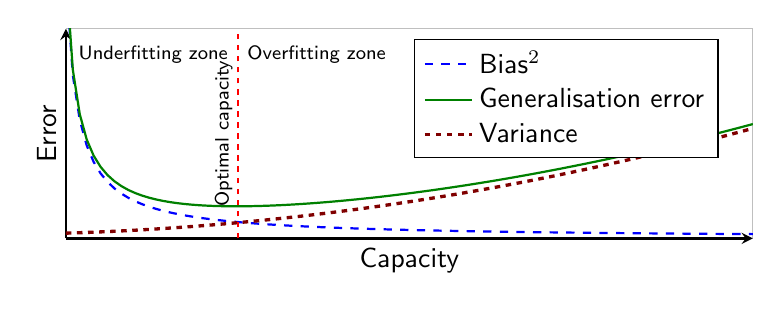
\begin{tikzpicture}[font=\sffamily\sansmath]

    \begin{axis}
        [
        xmin=0,
        xmax=2,
        ymin=0,
        ymax=2,
        xlabel=Capacity,
        ylabel=Error,
        ticks=none,
        xtick={2},
        ytick={2},
        xticklabels={\empty},
        yticklabels={\empty},
        ymajorgrids=true,
        xmajorgrids=true,
        samples=100,
        width=0.85\linewidth,
        height=0.35\linewidth,
        axis line style = thick,
        legend cell align={left},
        legend style={at={(0.95,0.95)},anchor=north east}
        ]
        \addplot[domain=0.00:2.0, blue, dashed, thick] {0.25/(3*x+0.1)};   % Error due to bias
        \addlegendentry{Bias$^2$}
        \addplot[domain=0.00:2.0, green!50!black, thick] {0.25/(3*x+0.1) + 0.1*x + 0.2 *x*x + 0.05};  % Generalisation error
        \addlegendentry{Generalisation error}
        \addplot[domain=0.00:2.0, red!50!black, dotted, very thick] {0.1*x + 0.2 *x*x + 0.05};  % Error due to variance
        \addlegendentry{Variance}
%      \addplot[domain=0.39:1.61,black] {3*(x-2)*x+3.8};  %Total error
        \addplot[dotted, red, thick] coordinates {(0.5,0) (0.5,2)};           %Optimum model complexity
%        \addplot[thin, <->] coordinates {(1.5,0.1) (1.5,0.65)};       %Optimum model complexity

        \node[OptimumStyle] at (axis cs:0.46,1.0) {Optimal capacity};
        \node[UnderfitStyle] at (axis cs:0.5,1.75) {Underfitting zone};
        \node[OverfitStyle] at (axis cs:0.5,1.75) {Overfitting zone};
%        \node[OverfitStyle] at (axis cs:1.5,0.33) {Generalisation gap};
%      \node[anchor=south west,text=Maroon] at (axis cs:1.4,0.4){Bias\textsuperscript{2}};
%      \node[anchor=north west,text=TealBlue] at (axis cs:1.4,0.85){Variance};
%      \node[anchor=south east,align=center] at (axis cs:1.5,1.5){Total\\error};
%        \legend{}
    \end{axis}
\end{tikzpicture}
%}

%\end{document}
    \captionsetup{format=hang} % hanging captions
    \caption{
        \textbf{The error source of a model evaluated using \gls{MSE}}. As the
        capacity of a model increases, the error source of the model transitions
        from bias dominated to variance dominated. The sum of both error sources
        yields the generalization error which is U-shaped. The optimal capacity
        of the model is exactly at this transition, where the bias error
        intersects the variance error. To the right of the transition, the model
        is overfitting and to the left, underfitting. This relationship is
        similar to that seen in \autoref{fig:capacity}.
    }
    \label{fig:bias-variance}
\end{figure}

%\subsubsection{Resubstitution}
%%%%%%%%%%%%%%%%%%%%%%%%%%%%%%%%%%%%%%%%%%%%%%%%%%%%%%%%%%%%%%%%%%%%%%%%%%%%%%%%

%\subsubsection{Holdout}
%%%%%%%%%%%%%%%%%%%%%%%%%%%%%%%%%%%%%%%%%%%%%%%%%%%%%%%%%%%%%%%%%%%%%%%%%%%%%%%%

\subsubsection{Cross-Validation}
%%%%%%%%%%%%%%%%%%%%%%%%%%%%%%%%%%%%%%%%%%%%%%%%%%%%%%%%%%%%%%%%%%%%%%%%%%%%%%%%
Cross-validation is often used for the assessment and optimization of
hyperparameters which improves a learning algorithm's ability to generalize on
unseen data. This is achieved through the separation of training folds from a
validation fold. The training fold is then separated into training data and
test data, while the validation fold is left out of the training procedure
entirely. The validation fold is then used to assess the performance of the
model on unseen data which has not been used to obtain the estimates of the
model parameters. A common way of performing cross-validation is to use a
\gls{KFCV}, where $k$ is the number of \textit{approximately
equal} folds that the data is separated into. The total dataset is then iterated
through, where each fold is used once as the validation fold and the remaining
folds are used as the training folds. The validation error is then calculated by
averaging the errors of all iterations. This is depicted in
\autoref{fig:kfold-cv}. \cite[p.~241-245]{hastie2009elements}


\begin{figure}[htbp]
    \centering
    % DEP
% \usetikzlibrary{matrix}

% ACK
% https://tex.stackexchange.com/questions/429451/k-fold-cross-validation-figure-using-tikz-or-table

\begin{tikzpicture}
    \matrix (M)
        [
        matrix of nodes,
        nodes={
            minimum height = 6mm,
            minimum width = 1.3cm,
            outer sep=0,
            anchor=center,
            draw
        },
        column 1/.style={nodes={draw=none}, minimum width = 4cm},
        column 5/.style={nodes={draw=gray}, dashed},
        column 7/.style={nodes={draw=none},minimum width = 1.0cm},
        row 4/.style={nodes={draw=none}},
        row sep=1mm,
        column sep=-\pgflinewidth,
        nodes in empty cells,
        e/.style={fill=yellow!10},
        n/.style={nodes={draw=none, fill=none}},
        ]
    {
        Iteration 1   & |[e]|  &        &        & $\ldots$ &        & \textrightarrow\;$e_1$ \\
        Iteration 2   &        & |[e]|  &        & $\ldots$ &        & \textrightarrow\;$e_2$ \\
        Iteration 3   &        &        & |[e]|  & $\ldots$ &        & \textrightarrow\;$e_3$ \\
              $\vdots$  & $\vdots$ & $\vdots$ & $\vdots$ & $\ddots$ & $\vdots$ & $\vdots$                \\
        Iteration $k$ &        &        &        & $\ldots$ & |[e]|  & \textrightarrow\;$e_k$ \\
    };
    \draw (M-1-2.north west) ++(0,2mm) coordinate (LT) edge[|<->|, >= latex] node[above]{Total number of folds, $k$} (LT-|M-1-6.north east);
%    \draw[decorate,decoration = {brace}] (bias-brace-down) --  (bias-brace-up);
    \draw[decorate,decoration = {brace, raise=0.5em, amplitude=0.5em}]
        (M-5-6.south east)
        -- node[below=1em, align=center] {Validation \\ fold}
        ([shift={(0.1em,0)}]M-5-6.south west);

    \draw[decorate,decoration = {brace, raise=0.5em, amplitude=0.5em}]
        ([shift={(-0.1em,0)}]M-5-5.south east)
        -- node[below=1em, align=center] {Training folds}
        (M-5-2.south west);

    \draw[decorate,decoration = {brace, raise=0.5em, amplitude=0.5em}]
        (M.north east)
        -- node[midway, right=1.5em] {$e=\frac{1}{k}\sum_{i=0}^k{e_i}$}
        (M.south east);

%    \matrix (L)
%        [
%        matrix of nodes,
%        right=of M,
%        nodes={
%            minimum height = 6mm,
%            minimum width = 1.5cm,
%            outer sep=0,
%            anchor=center,
%            draw
%        },
%        column 1/.style={nodes={draw=none}, minimum width = 4cm},
%        row sep=1mm,
%        column sep=-\pgflinewidth,
%        nodes in empty cells,
%        e/.style={fill=yellow!10}
%        ]
%    {
%        Training   &       \\
%        Validation & |[e]| \\
%    };

%    \node[east=of M.east] {
%    \hskip1em
%    \begin{tabular}[c]{|p{2em}|l}
%      \cline{1-1}
%      \ccell{0}{1}  & Training
%      \nextrow{1-1}
%      \ccell{1}{1}  & Validation\\
%      \cline{1-1}
%    \end{tabular}
%    }
\end{tikzpicture}
    \captionsetup{format=hang} % hanging captions
    \caption{
        $\bm{k}$\textbf{-fold cross-validation procedure:} (1) Dataset is divided into
        $k$-folds of roughly equal size. (2) Choose one fold randomly to be the
        holdout set then fit model on the remaining $k-1$ folds. (3) Iterate
        through the remaining $k-1$ folds, using each as the holdout set and
        record the error $e_i$ of the iteration. (4) Average the errors obtained
        over the $k$-folds.
    }
    \label{fig:kfold-cv}
\end{figure}

%\subsection{Challenges faced Machine Learning}
%%%%%%%%%%%%%%%%%%%%%%%%%%%%%%%%%%%%%%%%%%%%%%%%%%%%%%%%%%%%%%%%%%%%%%%%%%%%%%%%%
%Machine learning methods explored in the field of statistical learning have
%worked well in founding key concepts in machine learning and have been
%successful in a variety of important problems. They however fail to address
%human-like learning tasks such as speech recognition, object recognition, and
%character recognition. Many practitioners had started to believe that such
%complex learning tasks were not solvable using learning algorithms.
%
%
%\subsubsection{The curse of dimensionality}
%%%%%%%%%%%%%%%%%%%%%%%%%%%%%%%%%%%%%%%%%%%%%%%%%%%%%%%%%%%%%%%%%%%%%%%%%%%%%%%%%
%
%\subsubsection{Local constancy and smoothness regularization}
%%%%%%%%%%%%%%%%%%%%%%%%%%%%%%%%%%%%%%%%%%%%%%%%%%%%%%%%%%%%%%%%%%%%%%%%%%%%%%%%%
%
%\subsubsection{Manifold learning}
%%%%%%%%%%%%%%%%%%%%%%%%%%%%%%%%%%%%%%%%%%%%%%%%%%%%%%%%%%%%%%%%%%%%%%%%%%%%%%%%%

%\subsubsection{Leave-One-Out Cross-Validation (LOOCV)}
%%%%%%%%%%%%%%%%%%%%%%%%%%%%%%%%%%%%%%%%%%%%%%%%%%%%%%%%%%%%%%%%%%%%%%%%%%%%%%%%

%\subsubsection{Bootstrapping}
%%%%%%%%%%%%%%%%%%%%%%%%%%%%%%%%%%%%%%%%%%%%%%%%%%%%%%%%%%%%%%%%%%%%%%%%%%%%%%%%

%\subsection{Supervised}
%%%%%%%%%%%%%%%%%%%%%%%%%%%%%%%%%%%%%%%%%%%%%%%%%%%%%%%%%%%%%%%%%%%%%%%%%%%%%%%%


%%%%%%%%%%%%%%%%%%%%%%%%%%%%%%%%%%%%%%%%%%%%%%%%%%%%%%%%%%%%%%%%%%%%%%%%%%%%%%%%

\newpage\section{Deep Learning\label{sec:DL}}
%%%%%%%%%%%%%%%%%%%%%%%%%%%%%%%%%%%%%%%%%%%%%%%%%%%%%%%%%%%%%%%%%%%%%%%%%%%%%%%%
\Gls{DL} is a field of \gls{ML} that is primarily concerned with the learning of
representations of data. At the core of \gls{DL} is the use of \glspl{MLP}, used
to model these representations. \Glspl{MLP} are fully connected layers of
biologically inspired artifical neurons, also known as \textbf{perceptrons}. A
brief history are these biologically inspired models are covered in
\autoref{ssec:perceptrons} with adapted notation from the field of \gls{DL}.
Although not all practices in \gls{DL}, strictly speaking, make use of
\glspl{MLP}, they are a fundamental concept which must be understood in the
stepping stones towards concepts of higher complexity in the field.
\autoref{ssec:mlps} covers this concept, extending directly on their composite
component: perceptrons.

\Glspl{MLP} are also called \textbf{feedfoward} as information is propagated in
only a forward direction, as apposed to exhibiting \textbf{feedback} connections,
where intermediate computations are fed back into the network. When feedforward
networks are extended to include feedback connections, they are called
\textbf{\glspl{RNN}}. These types of networks excel at learning temporal
features, exhibiting a refined hypothesis space favouring sequenced information,
such as a series of chronological observations. \autoref{ssec:rnn} covers this
type of \gls{DNN}, and the prominent sub-type of \glspl{RNN}: \glspl{LSTM}.

One category of neural networks which are similar to \glspl{MLP}, popular in
contemporary research, are \glspl{CNN}. These \glspl{DNN} are essentially
\glspl{MLP} which omit the property of being fully connected, in favour of
refining the hypothesis space towards detection of spatially-related features.

The main difference between a \gls{NN} and a
traditional \gls{ML} algorithm is that the neural network is a function of the
data, rather than the data itself.

\subsection{Brief History of the Perceptron\label{ssec:perceptrons}}
%%%%%%%%%%%%%%%%%%%%%%%%%%%%%%%%%%%%%%%%%%%%%%%%%%%%%%%%%%%%%%%%%%%%%%%%%%%%%%%%

The McCullock-Pitts neuron, an earlier iteration of an artificial neuron, was
proposed by McCulloch and Pitts in the field of neuroscience in 1943
\cite{McCulloch1943}. Their work contended that neurons with a binary activation
function were analogous to first order logic sentences. The perception of
artifical neurons changed with Hebb's work in 1949, where he proposed an idea
which has come to be known as Hebb's rule:

\begin{fancyquotes}
    Let us assume that the persistence or repetition of a reverberatory activity
    (or ``trace") tends to induce lasting cellular changes that add to its
    stability. [...] When an axon of cell A is near enough to excite a cell B
    and repeatedly or persistently takes part in firing it, some growth process
    or metabolic change takes place in one or both cells such that A’s
    efficiency, as one of the cells firing B, is increased. \cite{10.1007/978-3-642-70911-1_15}
\end{fancyquotes}

This theory is often summaraized as \textit{``Cells that fires together, wire
together"} \cite{doi:10.1126/science.7912852}, which persists today in the
gradient-based learning at the core of contemporary \gls{DL}. The perceptron was
proposed by Rosenblatt \cite{Rosenblatt_1957_6098} in his technical report
funded by the United States Office of Naval Research
\cite{doi:10.1177/030631296026003005} in 1957. Rosenblatt incorporated Hebb's
findings into the McCullock-Pitts neuron.

The \textit{perceptron} is arguably the most fundamental concept in deep
learning, describing a mathematical model of a biological neuron. There are two
different sets of notation which exist when dealing with the bias of a
perceptron. One involves the inclusion of a unit constant in the input vector
$\mathbf{x}$, with the bias being specified by the value of the first weight
$w_0$. An alternative notation exists which treats the bias as a standalone
value $b$. The latter notation will be used, as it is the preferred notation in
contemporary deep learning research. The notation defining the mapping of a
perceptron is then: $f(\gls{ml:x};\gls{w_vec},
\gls{b})=\gls{ml:x}^T\gls{w_vec}+\gls{b}$;
$\gls{ml:x}\in\gls{set:R}^{\gls{ml:n_x}}$,
$\gls{w_vec}\in\gls{set:R}^{\gls{ml:n_x}}$, $\gls{b}\in\gls{set:R}$. Furthermore
the model parameters, \gls{ml:theta}, as introduced in
\autoref{sec:capoverunder}, are defined by the union of the bias and weight
vectors: $\gls{ml:theta}=\{\gls{w_vec},\gls{b}\}$.
\begin{figure}[htbp]
    \centering
    % MIT License
%
% Copyright (c) 2021 Geoffrey H. Garrett
%
% Permission is hereby granted, free of charge, to any person obtaining a copy
% of this software and associated documentation files (the "Software"), to deal
% in the Software without restriction, including without limitation the rights
% to use, copy, modify, merge, publish, distribute, sublicense, and/or sell
% copies of the Software, and to permit persons to whom the Software is
% furnished to do so, subject to the following conditions:
%
% The above copyright notice and this permission notice shall be included in all
% copies or substantial portions of the Software.
%
% THE SOFTWARE IS PROVIDED "AS IS", WITHOUT WARRANTY OF ANY KIND, EXPRESS OR
% IMPLIED, INCLUDING BUT NOT LIMITED TO THE WARRANTIES OF MERCHANTABILITY,
% FITNESS FOR A PARTICULAR PURPOSE AND NONINFRINGEMENT. IN NO EVENT SHALL THE
% AUTHORS OR COPYRIGHT HOLDERS BE LIABLE FOR ANY CLAIM, DAMAGES OR OTHER
% LIABILITY, WHETHER IN AN ACTION OF CONTRACT, TORT OR OTHERWISE, ARISING FROM,
% OUT OF OR IN CONNECTION WITH THE SOFTWARE OR THE USE OR OTHER DEALINGS IN THE
% SOFTWARE.

%%%%%%%%%%%%%%%%%%%%%%%%%%%%%%%%%%%%%%%%%%%%%%%%%%%%%%%%%%%%%%%%%%%%%%%%%%%%%%%
% ACKNOWLEDGEMENTS
%%%%%%%%%%%%%%%%%%%%%%%%%%%%%%%%%%%%%%%%%%%%%%%%%%%%%%%%%%%%%%%%%%%%%%%%%%%%%%%
% Design and implementation of this diagram was inspired and adapted from:
% https://tex.stackexchange.com/questions/104334/tikz-diagram-of-a-perceptron

%%%%%%%%%%%%%%%%%%%%%%%%%%%%%%%%%%%%%%%%%%%%%%%%%%%%%%%%%%%%%%%%%%%%%%%%%%%%%%%
% DEPENDENCIES
%%%%%%%%%%%%%%%%%%%%%%%%%%%%%%%%%%%%%%%%%%%%%%%%%%%%%%%%%%%%%%%%%%%%%%%%%%%%%%%
%\usepackage{tikz}
%\usetikzlibrary{decorations.pathreplacing}    % for TikZ braces
%\usetikzlibrary{positioning}                  % for TikZ relative positioning

%%%%%%%%%%%%%%%%%%%%%%%%%%%%%%%%%%%%%%%%%%%%%%%%%%%%%%%%%%%%%%%%%%%%%%%%%%%%%%%
% USER STYLING
%%%%%%%%%%%%%%%%%%%%%%%%%%%%%%%%%%%%%%%%%%%%%%%%%%%%%%%%%%%%%%%%%%%%%%%%%%%%%%%

% TikZ node design.
\tikzset{basic/.style={draw,text width=1em,text badly centered}}
\tikzset{input/.style={}}
\tikzset{output/.style={}}
\tikzset{weight/.style={basic,circle}}
\tikzset{hidden/.style={basic,circle}}
\tikzset{function/.style={basic,circle}}
\def\layersep{3em}
\def\transferx{9em}
\def\hiddenx{7em}
\def\hiddenxn{12em}

% Labels and symbols.
\def\activationlabel{activation function}  % activation function label
\def\activationsymbol{$\phi$}              % activation function symbol
\def\transferlabel{transfer function}      % transfer function label
\def\transfersymbol{$\sum$}                % transfer function symbol
\def\outputsymbol{$y$}                     % output symbol
\def\inputsymbol{$x$}                      % input symbol
\def\inputvecsymbol{$\mathbf{x}$}          % input vector symbol
\def\weightslabel{weights}                 % input vector symbol
\def\biassymbol{$b$}                       % bias symbol

\def\sep{4em}
\def\L{\gls{L}}       % number of hidden layers
\def\y{\gls{y_true}}  % output vector
\def\x{\gls{ml:x}}    % input vector
\def\h{\gls{a_vec}}   % hidden output
\def\nx{\gls{np:dim}[_\gls{fn:in}]}   % hidden output
\def\ny{\gls{np:dim}[_\gls{fn:out}]}   % hidden output
\def\a{\gls{dl:a}}   % hidden output
\def\z{\gls{dl:z}}   % hidden output

%%%%%%%%%%%%%%%%%%%%%%%%%%%%%%%%%%%%%%%%%%%%%%%%%%%%%%%%%%%%%%%%%%%%%%%%%%%%%%%
% TIKZ PICTURE
%%%%%%%%%%%%%%%%%%%%%%%%%%%%%%%%%%%%%%%%%%%%%%%%%%%%%%%%%%%%%%%%%%%%%%%%%%%%%%%
\begin{tikzpicture}

    \node[function] at ({\transferx}, -{int(2)})  (transfer) {\transfersymbol};
    \node[function, right=3em of transfer] (activation) {\activationsymbol};
    \node[below of=activation,font=\scriptsize,text width=3em] {\activationlabel};
    \node[below of=transfer,font=\scriptsize,text width=3em] {\transferlabel};
    \node[output, right=\layersep of activation] (output) {\outputsymbol};
    \path[draw,->] (transfer) -- node[above] {\z} (activation);
    \path[draw,->] (activation) -- node[above] {\a} (output);
%    \path[draw,->] (activation)(output);

    % Iterate through each row of units.
    \foreach \n [evaluate=\n as \p using {int(\n-1)}] in {0,1,2,3,4} {
        \ifnum \n=0
            \node[input] at (0, -\n) (X-\n) {$1$};
            \node[weight] at (\layersep, -\n) (W-\n) {$w_\n$};
        \else \ifnum \n=3
            \node[] at (0, -\n) (X-\n) {$\vdots$};
            \node[] at (\layersep, -\n) (W-\n) {$\vdots$};
        \else \ifnum \n=4
            \node[input] at (0, -\n) (X-\n) {$x_{\nx}$};
            \node[weight,label={[xshift=-0.0em]center:$w_{\nx}$}] at (\layersep, -\n) (W-\n) {\phantom{$w_{\nx}$}};
        \else
            \node[input] at (0, -\n) (X-\n) {$x_\n$};
            \node[weight] at (\layersep, -\n) (W-\n) {$w_\n$};
        \fi
        \fi
        \fi

        % Arrow from input to weight.
        \ifnum \n=3
        \else
            \path[draw,->] (X-\n) -- (W-\n);
                        \path[draw,->] (W-\n) -- (transfer);
        \fi

    }

    % Brace for bias.
    \node[left=1em of X-0] (bias-brace) {};
    \node[above=1em of bias-brace] (bias-brace-up) {};
    \node[below=1em of bias-brace] (bias-brace-down) {};
    \draw[decorate,decoration = {brace}] (bias-brace-down) --  (bias-brace-up);
    \node[left of=bias-brace,font=\scriptsize] {bias, \biassymbol};

    % Brace for input.
    \node[below=10em of bias-brace-down] (input-brace-down) {};
    \node[below=5em of bias-brace-down] (input-brace) {};
    \draw[decorate,decoration = {brace}] (input-brace-down) --  (bias-brace-down);
    \node[left of=input-brace,font=\scriptsize] {inputs, \inputvecsymbol};

    % Weights label.
    \node[below of=W-4,font=\scriptsize] {\weightslabel};

\end{tikzpicture}

    \captionsetup{format=hang} % hanging captions
    \caption{
        \textbf{Generalized illustration of a perceptron.} The mapping is
        defined by $f(\gls{ml:x};\gls{w_vec},
        \gls{b})=\gls{ml:x}^T\gls{w_vec}+\gls{b}$ where
        $\{\gls{w_vec},\gls{b}\}=\gls{ml:theta}$. The original formulation of
        the perceptron \cite{Rosenblatt_1957_6098} was intended to output a
        binary value, using a threshold step function, for classification
        purposes. The actual activation function \gls{dl:activation} has been
        generalized in order to relate the concept to modern deep learning
        techniques.
    }
    \label{fig:perceptron}
\end{figure}

\begin{equation}
    a=g\bigg(\sum_{k=0}^{\gls{ml:n_x}}{w_k}x_k + b\bigg)=g(z)
\end{equation}


%Rosenblatt's incorporated the model of  Rosenblatt
%incorporated the findings of Hebb \cite{10.1007/978-3-642-70911-1_15} into the
%model proposed by A set of inputs \gls{ml:x} would be weighted before being
%passed through a threshold step activation function \gls{dl:activation}.
%\autoref{fig:perceptron} shows a more general formulation which applies to the
%field of deep learning, with any activation function, \gls{dl:activation},
%mimicking a level of excitation akin to a biological neuron in response to its
%stimulus \gls{ml:x}.

\begin{figure}[!htp]
    \centering
    \begin{subfigure}[b]{0.70\textwidth}
        \centering
        % MIT License
%
% Copyright (c) 2021 Geoffrey H. Garrett
%
% Permission is hereby granted, free of charge, to any person obtaining a copy
% of this software and associated documentation files (the "Software"), to deal
% in the Software without restriction, including without limitation the rights
% to use, copy, modify, merge, publish, distribute, sublicense, and/or sell
% copies of the Software, and to permit persons to whom the Software is
% furnished to do so, subject to the following conditions:
%
% The above copyright notice and this permission notice shall be included in all
% copies or substantial portions of the Software.
%
% THE SOFTWARE IS PROVIDED "AS IS", WITHOUT WARRANTY OF ANY KIND, EXPRESS OR
% IMPLIED, INCLUDING BUT NOT LIMITED TO THE WARRANTIES OF MERCHANTABILITY,
% FITNESS FOR A PARTICULAR PURPOSE AND NONINFRINGEMENT. IN NO EVENT SHALL THE
% AUTHORS OR COPYRIGHT HOLDERS BE LIABLE FOR ANY CLAIM, DAMAGES OR OTHER
% LIABILITY, WHETHER IN AN ACTION OF CONTRACT, TORT OR OTHERWISE, ARISING FROM,
% OUT OF OR IN CONNECTION WITH THE SOFTWARE OR THE USE OR OTHER DEALINGS IN THE
% SOFTWARE.

%%%%%%%%%%%%%%%%%%%%%%%%%%%%%%%%%%%%%%%%%%%%%%%%%%%%%%%%%%%%%%%%%%%%%%%%%%%%%%%
% ACKNOWLEDGEMENTS
%%%%%%%%%%%%%%%%%%%%%%%%%%%%%%%%%%%%%%%%%%%%%%%%%%%%%%%%%%%%%%%%%%%%%%%%%%%%%%%
% Design and implementation of this diagram was inspired and adapted from:
% https://tex.stackexchange.com/questions/104334/tikz-diagram-of-a-perceptron

%%%%%%%%%%%%%%%%%%%%%%%%%%%%%%%%%%%%%%%%%%%%%%%%%%%%%%%%%%%%%%%%%%%%%%%%%%%%%%%
% DEPENDENCIES
%%%%%%%%%%%%%%%%%%%%%%%%%%%%%%%%%%%%%%%%%%%%%%%%%%%%%%%%%%%%%%%%%%%%%%%%%%%%%%%
%\usepackage{tikz}
%\usetikzlibrary{decorations.pathreplacing}    % for TikZ braces
%\usetikzlibrary{positioning}                  % for TikZ relative positioning

%%%%%%%%%%%%%%%%%%%%%%%%%%%%%%%%%%%%%%%%%%%%%%%%%%%%%%%%%%%%%%%%%%%%%%%%%%%%%%%
% USER STYLING
%%%%%%%%%%%%%%%%%%%%%%%%%%%%%%%%%%%%%%%%%%%%%%%%%%%%%%%%%%%%%%%%%%%%%%%%%%%%%%%

% TikZ node design.
\tikzset{basic/.style={draw,text width=1em,text badly centered}}
\tikzset{input/.style={}}
\tikzset{output/.style={}}
\tikzset{weight/.style={basic,circle}}
\tikzset{hidden/.style={basic,circle}}
\tikzset{function/.style={basic,circle}}
\def\layersep{3em}
\def\transferx{9em}
\def\hiddenx{7em}
\def\hiddenxn{12em}

% Labels and symbols.
\def\activationlabel{threshold step}  % activation function label
\def\activationsymbol{$H$}              % activation function symbol
\def\transferlabel{sum}      % transfer function label
\def\transfersymbol{$\sum$}                % transfer function symbol
\def\outputsymbol{$\text{AND}(x_1, x_2)$}                     % output symbol
\def\inputsymbol{$x$}                      % input symbol
\def\inputvecsymbol{$\mathbf{x}$}          % input vector symbol
\def\weightslabel{weights}                 % input vector symbol
\def\biassymbol{$b$}                       % bias symbol

\def\sep{4em}
\def\L{\gls{L}}       % number of hidden layers
\def\y{\gls{y_true}}  % output vector
\def\x{\gls{ml:x}}    % input vector
\def\h{\gls{a_vec}}   % hidden output
\def\nx{\gls{ml:n_x}}   % hidden output
\def\ny{\gls{ml:n_y}}   % hidden output
\def\z{\gls{dl:z}}   % hidden output
\def\a{\gls{dl:a}}   % hidden output

%%%%%%%%%%%%%%%%%%%%%%%%%%%%%%%%%%%%%%%%%%%%%%%%%%%%%%%%%%%%%%%%%%%%%%%%%%%%%%%
% TIKZ PICTURE
%%%%%%%%%%%%%%%%%%%%%%%%%%%%%%%%%%%%%%%%%%%%%%%%%%%%%%%%%%%%%%%%%%%%%%%%%%%%%%%
\begin{tikzpicture}

    \node[function] at ({\transferx}, -{int(2)})  (transfer) {\transfersymbol};
    \node[function, right=3em of transfer] (activation) {\activationsymbol};
    \node[below of=activation,font=\scriptsize,text width=3em] {\activationlabel};
    \node[below of=transfer,font=\scriptsize,text width=3em] {\transferlabel};
    \node[output, right=\layersep of activation] (output) {\outputsymbol};
    \path[draw,->] (transfer) -- node[above] {\z} (activation);
    \path[draw,->] (activation) -- node[above] {\a} (output);

    \node[input] at (0, -1) (X-1) {$1$};
    \def\wone{$-1$}
    \node[weight, label={[xshift=-0.0em]center:\wone}] at (\layersep, -1) (W-1) {\phantom{\wone}};

    \node[input] at (0, -2) (X-2) {$x_1$};
    \def\wtwo{$1$}
    \node[weight, label={[xshift=-0.0em]center:\wtwo}] at (\layersep, -2) (W-2) {\phantom{\wtwo}};

    \node[input] at (0, -3) (X-3) {$x_2$};
    \def\wthree{$1$}
    \node[weight, label={[xshift=-0.0em]center:\wthree}] at (\layersep, -3) (W-3) {\phantom{\wthree}};

    \path[draw,->] (X-1) -- (W-1);
    \path[draw,->] (X-2) -- (W-2);
    \path[draw,->] (X-3) -- (W-3);
    \path[draw,->] (W-1) -- (transfer);
    \path[draw,->] (W-2) -- (transfer);
    \path[draw,->] (W-3) -- (transfer);

    % Brace for bias.
    \node[left=1em of X-1] (bias-brace) {};
    \node[above=1em of bias-brace] (bias-brace-up) {};
    \node[below=1em of bias-brace] (bias-brace-down) {};
    \draw[decorate,decoration = {brace}] (bias-brace-down) --  (bias-brace-up);
    \node[left of=bias-brace,font=\scriptsize] {bias, \biassymbol};

    % Brace for input.
    \node[below=4.5em of bias-brace-down] (input-brace-down) {};
    \node[below=2.25em of bias-brace-down] (input-brace) {};
    \draw[decorate,decoration = {brace}] (input-brace-down) --  (bias-brace-down);
    \node[left of=input-brace,font=\scriptsize] {inputs, \inputvecsymbol};

    % Weights label.
    \node[below of=W-3,font=\scriptsize] {\weightslabel};

\end{tikzpicture}

        \captionsetup{format=hang} % hanging captions
        \subcaption{Perceptron mapping}
        \label{fig:perceptron:and:mapping}
    \end{subfigure}\hfil
    \begin{subfigure}[b]{0.29\textwidth}
        \centering
        \renewcommand{\arraystretch}{1.5}
        \begin{tabular}{C{0.1\linewidth}C{0.1\linewidth}|C{0.1\linewidth}}
            \hline
            $x_1$ & $x_2$ & $y$ \\ \hline
            0     & 0     & 0   \\
            0     & 1     & 0   \\
            1     & 0     & 0   \\
            1     & 1     & 1
        \end{tabular}
        \vspace{0.5cm}
        \subcaption{Truth table}
        \label{fig:perceptron:and:truth}
    \end{subfigure}\hfil
    \captionsetup{format=hang} % hanging captions
    \caption{
        \textbf{Truth table of the AND logic gate.}
    }
    \label{fig:perceptron:and}
\end{figure}



Rosenblatt's statements caused an unfortunate controversy in the fledgling field
of \gls{AI}. According to the New York Times, he reported the perceptron to be
\textit{``the embryo of an electronic computer that [the Navy] expects will be
able to walk, talk, see, write, reproduce itself and be conscious of its
existence."} \cite{Olazaran1996} The backlash from the \gls{AI} community

\subsubsection{Perceptrons and Logic Gates}




In its original form, the perceptron was used as a supervised learning method
for binary classifiers.

The primary criticism of the perceptron came in 1969 from Minsky and Papert
\cite{minsky69perceptrons}, where it was shown that the perceptron could only
solve \textit{linearly separable} functions, and failed to solve the XOR and
NXOR functions. They claimed that the work being done in this area was doomed to
failure due to these limitations, resulting in little subsequent research until
about the 1980's.


%
%\newpage
\newpage

\subsection{Multi-layer perceptrons\label{ssec:mlps}}
%%%%%%%%%%%%%%%%%%%%%%%%%%%%%%%%%%%%%%%%%%%%%%%%%%%%%%%%%%%%%%%%%%%%%%%%%%%%%%%%%
\Gls{MLPs}, otherwise known as \textbf{artificial neural networks} or
\textbf{feedforward neural networks}, are the fundamental models of \gls{DL}.
These models are biologically inspired, and make direct use of the concept of
the perceptron discussed in \autoref{ssec:perceptrons}. The primary extensions
involve the use of a variety of activation functions other than the threshold
step, and multiple layers of fully connected perceptrons, often referred to as
\textbf{neurons} or \textbf{units}. \gls{MLPs} are characterized as being
\textbf{fully-connected} which means that all the units in a layer are connected
to all units in the next. These models are often referred to as \textbf{deep
feedfoward networks} by virtue of having \textit{several} hidden layers. Note
that there is no universally accepted definition of what integer values of
perceptron layers \gls{dl:L} constitute deep and shallow networks, but generally
speaking: a shallow network will usually have one hidden layer and a deep
network will have several hidden layers. The mapping of an \gls{MLP} is defined
by $\gls{y_pred}=f(\gls{ml:x}; \gls{theta})$;
$\gls{ml:x}\in\gls{set:R}^{\gls{ml:n_x}}$;
$\gls{y_pred}\in\gls{set:R}^{\gls{ml:n_y}}$.

\begin{figure}[htp]
    \centering
    % MIT License
%
% Copyright (c) 2021 Geoffrey H. Garrett
%
% Permission is hereby granted, free of charge, to any person obtaining a copy
% of this software and associated documentation files (the "Software"), to deal
% in the Software without restriction, including without limitation the rights
% to use, copy, modify, merge, publish, distribute, sublicense, and/or sell
% copies of the Software, and to permit persons to whom the Software is
% furnished to do so, subject to the following conditions:
%
% The above copyright notice and this permission notice shall be included in all
% copies or substantial portions of the Software.
%
% THE SOFTWARE IS PROVIDED "AS IS", WITHOUT WARRANTY OF ANY KIND, EXPRESS OR
% IMPLIED, INCLUDING BUT NOT LIMITED TO THE WARRANTIES OF MERCHANTABILITY,
% FITNESS FOR A PARTICULAR PURPOSE AND NONINFRINGEMENT. IN NO EVENT SHALL THE
% AUTHORS OR COPYRIGHT HOLDERS BE LIABLE FOR ANY CLAIM, DAMAGES OR OTHER
% LIABILITY, WHETHER IN AN ACTION OF CONTRACT, TORT OR OTHERWISE, ARISING FROM,
% OUT OF OR IN CONNECTION WITH THE SOFTWARE OR THE USE OR OTHER DEALINGS IN THE
% SOFTWARE.

%%%%%%%%%%%%%%%%%%%%%%%%%%%%%%%%%%%%%%%%%%%%%%%%%%%%%%%%%%%%%%%%%%%%%%%%%%%%%%%
% ACKNOWLEDGEMENTS
%%%%%%%%%%%%%%%%%%%%%%%%%%%%%%%%%%%%%%%%%%%%%%%%%%%%%%%%%%%%%%%%%%%%%%%%%%%%%%%
% Adapted from:
% https://www.researchgate.net/figure/The-agent-environment-interaction-in-reinforcement-learning_fig1_328494763

%%%%%%%%%%%%%%%%%%%%%%%%%%%%%%%%%%%%%%%%%%%%%%%%%%%%%%%%%%%%%%%%%%%%%%%%%%%%%%%
% DEPENDENCIES
%%%%%%%%%%%%%%%%%%%%%%%%%%%%%%%%%%%%%%%%%%%%%%%%%%%%%%%%%%%%%%%%%%%%%%%%%%%%%%%
%\usepackage{tikz}
%\usetikzlibrary{decorations.pathreplacing}    % for TikZ braces
%\usetikzlibrary{positioning}                  % for TikZ relative positioning

%%%%%%%%%%%%%%%%%%%%%%%%%%%%%%%%%%%%%%%%%%%%%%%%%%%%%%%%%%%%%%%%%%%%%%%%%%%%%%%
% USER STYLING
%%%%%%%%%%%%%%%%%%%%%%%%%%%%%%%%%%%%%%%%%%%%%%%%%%%%%%%%%%%%%%%%%%%%%%%%%%%%%%%

% TikZ node design.
\tikzset{basic/.style={draw,text width=1em,text badly centered}}
\tikzset{input/.style={basic, fill=green!25, circle}}
\tikzset{output/.style={basic, fill=blue!25, circle}}
\tikzset{weight/.style={basic,circle}}
\tikzset{hidden/.style={basic,circle}}
\tikzset{function/.style={basic,circle}}
\def\layersep{3em}
\def\transferx{9em}
\def\hiddenx{7em}
\def\hiddenxn{12em}


\def\sep{4em}
\def\L{\gls{L}}       % number of hidden layers
\def\y{\gls{y_true}}  % output vector
\def\x{\gls{ml:x}}    % input vector
\def\h{\gls{a_vec}}   % hidden output
\def\nx{\gls{ml:n_x}}   % hidden output
\def\ny{\gls{ml:n_y}}   % hidden output


%%%%%%%%%%%%%%%%%%%%%%%%%%%%%%%%%%%%%%%%%%%%%%%%%%%%%%%%%%%%%%%%%%%%%%%%%%%%%%%
% TIKZ PICTURE
%%%%%%%%%%%%%%%%%%%%%%%%%%%%%%%%%%%%%%%%%%%%%%%%%%%%%%%%%%%%%%%%%%%%%%%%%%%%%%%
\begin{tikzpicture}
    \usetikzlibrary{decorations.pathreplacing}    % for TikZ braces
    \usetikzlibrary{positioning}                  % for TikZ relative positioning

    % input
    \foreach \n/\p in {0/1,1/2,2/3,3/4,4/5} {
        \ifnum \n=3
            % dots layer
            \node[] at (0, -\n) (X_\n) {$\vdots$};
            \node[] at (\hiddenx, -\n) (H1_\n) {$\vdots$};
            \node[right of=H1_\n] (M-\n) {$\ddots$};
            \node[below of=H1_2] (H2_\n) {$\vdots$};
            \node[below of=H2_2] (H2_\n) {$\vdots$};
            \node[right=5.7em of H2_\n] (Y_\n) {$\vdots$};
        \else
        \ifnum \n=4
            % n layer
            \node[input] at (0, -\n) (X_\n) {};
            \node[left of=X_\n] (I_\n) {$x_{\nx}$};
            \path[draw,->] (I_\n) -- (X_\n);
            \node[hidden] at (\hiddenx, -\n) (H1_\n) {}; %{$h_{n, 1}$};
            \node[right of= H1_\n] (M-\n) {$\ldots$};
            \node[hidden, right of= M-\n] (H2_\n) {}; % {$h_{n, m}$};
            \node[output, right= 5em of H2_\n] (Y_\n) {}; % {$h_{n, m}$};
            \node[right of=Y_\n] (O_\n) {$y_{\ny}$};
            \path[draw,->] (Y_\n) -- (O_\n);
        \else
            \node[input] at (0, -{\n}) (X_\n) {};
            \node[left of=X_\n] (I_\n) {$x_{\p}$};
            \path[draw,->] (I_\n) -- (X_\n);
            \node[hidden] at (\hiddenx, -\n) (H1_\n) {};%{$h_{\n, 1}$};
            \node[right of=H1_\n] (M-\n) {$\ldots$};
            \node[hidden, right of=M-\n] (H2_\n) {};% {$h_{\n, m}$};
            \node[output, right= 5em of H2_\n] (Y_\n) {}; % {$h_{n, m}$};
            \node[right of=Y_\n] (O_\n) {$y_\p$};
            \path[draw,->] (Y_\n) -- (O_\n);
        \fi
        \fi
    }

    % input layer connected to first hidden layer
    \foreach \j in {0,1,2,4} {
        \foreach \n in {0,1,2,4} {
            \path[draw,->] (X_\n) -- (H1_\j);
        }
    }

    % second hidden layer connected to output layer
    \foreach \j in {0,1,2,4} {
        \foreach \n in {0,1,2,4} {
            \path[draw,->] (H2_\n) -- (Y_\j);
        }
    }

    % labels
    \node[below of=X_4,font=\scriptsize, align=center] {input\\layer};
    \node[below of=Y_4,font=\scriptsize, align=center] {output\\layer};

    % brace for hidden layers
    \node[below=1em of M-4] (hidden-brace) {};
    \node[right=3em of hidden-brace] (hidden-brace-right) {};
    \node[left=3em of hidden-brace] (hidden-brace-left) {};
    \draw [decorate,decoration = {brace}] (hidden-brace-right) --  (hidden-brace-left);
    \node[below=0.5em of hidden-brace,font=\scriptsize] (hlayer) {hidden layer(s)};

\end{tikzpicture}


    \captionsetup{format=hang} % hanging captions
    \caption{
        \textbf{Generalized form of an \gls{MLP}}. Each layer, \textbf{excluding
        the input layer}, has associated weights, biases and activation
        functions. Furthermore, the layers are characterized as being
        \textbf{fully-connected}.
    }
    \label{fig:mlp}
\end{figure}

\autoref{fig:mlp} depicts the generalized concept of the \gls{MLP}. There are
three distinct types of layers: hidden, input, and output, for which
there is only one of each for the latter two. The input layer is simply the
input vector $\gls{ml:x}$, which does not have any weights, bias or activation
function associated to it.

\begin{figure}[htp]
    \centering
    % MIT License
%
% Copyright (c) 2021 Geoffrey H. Garrett
%
% Permission is hereby granted, free of charge, to any person obtaining a copy
% of this software and associated documentation files (the "Software"), to deal
% in the Software without restriction, including without limitation the rights
% to use, copy, modify, merge, publish, distribute, sublicense, and/or sell
% copies of the Software, and to permit persons to whom the Software is
% furnished to do so, subject to the following conditions:
%
% The above copyright notice and this permission notice shall be included in all
% copies or substantial portions of the Software.
%
% THE SOFTWARE IS PROVIDED "AS IS", WITHOUT WARRANTY OF ANY KIND, EXPRESS OR
% IMPLIED, INCLUDING BUT NOT LIMITED TO THE WARRANTIES OF MERCHANTABILITY,
% FITNESS FOR A PARTICULAR PURPOSE AND NONINFRINGEMENT. IN NO EVENT SHALL THE
% AUTHORS OR COPYRIGHT HOLDERS BE LIABLE FOR ANY CLAIM, DAMAGES OR OTHER
% LIABILITY, WHETHER IN AN ACTION OF CONTRACT, TORT OR OTHERWISE, ARISING FROM,
% OUT OF OR IN CONNECTION WITH THE SOFTWARE OR THE USE OR OTHER DEALINGS IN THE
% SOFTWARE.

%%%%%%%%%%%%%%%%%%%%%%%%%%%%%%%%%%%%%%%%%%%%%%%%%%%%%%%%%%%%%%%%%%%%%%%%%%%%%%%
% DEPENDENCIES
%%%%%%%%%%%%%%%%%%%%%%%%%%%%%%%%%%%%%%%%%%%%%%%%%%%%%%%%%%%%%%%%%%%%%%%%%%%%%%%
%\usepackage{tikz}
%\usetikzlibrary{decorations.pathreplacing}    % for TikZ braces
%\usetikzlibrary{positioning}                  % for TikZ relative positioning

%%%%%%%%%%%%%%%%%%%%%%%%%%%%%%%%%%%%%%%%%%%%%%%%%%%%%%%%%%%%%%%%%%%%%%%%%%%%%%%
% USER STYLING
%%%%%%%%%%%%%%%%%%%%%%%%%%%%%%%%%%%%%%%%%%%%%%%%%%%%%%%%%%%%%%%%%%%%%%%%%%%%%%%

% TikZ node design.
\tikzset{basic/.style={draw,text badly centered}}
\tikzset{input/.style={basic,minimum width=1.2cm, fill=green!25, circle}}
\tikzset{output/.style={basic,minimum width=1.2cm, fill=blue!25, circle}}
\tikzset{weight/.style={basic,circle}}
\tikzset{hidden/.style={basic,circle, minimum width=1.2cm}}
\tikzset{function/.style={basic,circle}}

\def\sep{4em}
\def\L{\gls{L}}       % number of hidden layers
\def\y{\gls{y_pred}}  % output vector
\def\x{\gls{ml:x}}    % input vector
\def\h{\gls{a_vec}}   % hidden output

%%%%%%%%%%%%%%%%%%%%%%%%%%%%%%%%%%%%%%%%%%%%%%%%%%%%%%%%%%%%%%%%%%%%%%%%%%%%%%%
% TIKZ PICTURE
%%%%%%%%%%%%%%%%%%%%%%%%%%%%%%%%%%%%%%%%%%%%%%%%%%%%%%%%%%%%%%%%%%%%%%%%%%%%%%%
\begin{tikzpicture}
    \node[input, label={[xshift=-0.0em]center:\gls{dl:a:vec:0}}] (X) {\phantom{\gls{dl:a:vec:1}}};
    \node[, left=1.5em of X] (in) {$\bm{x}$};

    \node[hidden, right=\sep of X, label={[xshift=-0.0em]center:\gls{dl:a:vec:1}}] (H1) {\phantom{\gls{dl:a:vec:1}}};
    \node[hidden, right=\sep of H1, label={[xshift=-0.0em]center:\gls{dl:a:vec:Lm1}}] (H2) {\phantom{\gls{dl:a:vec:Lm1}}};
    \node[output, right=\sep of H2,  label={[xshift=-0.0em]center:\gls{dl:a:vec:L}}] (Y) {\phantom{\gls{dl:a:vec:L}}};
    \node[, right=1.5em of Y] (out) {$\bm{\hat{y}}$};

    \path[draw,->] (in) -- (X);
    \path[draw,->] (X) -- (H1);
    \node[right=0.8em of H1] (M) {$\ldots$};
    \path[draw,->] (H2) -- (Y);
    \path[draw,->] (Y) -- (out);
\end{tikzpicture}


    \captionsetup{format=hang} % hanging captions
    \caption{
        \textbf{Generalized vector form of an \gls{MLP}}. By notation, the
        input layer is denoted by $\gls{dl:a:vec:0}$ or $\gls{ml:x}$, the
        output layer is denoted by $\gls{dl:a:vec:L}$ or $\gls{y_pred}$, and the
        hidden layers as $\gls{dl:a:vec:l}\;\forall{}\;l\in\{1,...,\gls{dl:L}-1\}$.
    }
    \label{fig:mlp-vec}
\end{figure}

\autoref{fig:mlp} and \autoref{fig:mlp-vec} are equivalent and introduce the
notation used for the variables of the network. The vector form of the
$l^\text{th}$ layer's activation variable is given by:

\begin{equation}
    \gls{dl:a:vec:l}
    = \gls{dl:g:l} \bigg(\gls{dl:w:l}^\text{T} \gls{dl:a:vec:lm1} + \gls{dl:b:l} \bigg)
    = \gls{dl:g:l}(\gls{dl:z:vec:l});
    \label{eq:mlp:a:vec}
\end{equation}

In the next section, where backpropagation is discussed, the following
scalar form of the activation will be used when deriving the expressions
used in the backpropagation algorithm:

\begin{equation}
    \gls{dl:a:l:j}
    = \gls{dl:g:l} \bigg(\sum_{k=0}^{\gls{dl:nh:lm1}} \gls{dl:w:l:jk} \gls{dl:a:lm1:k} + \gls{dl:b:l:j} \bigg)
    = \gls{dl:g:l}(\gls{dl:z:l:j});
    \label{eq:mlp:a}
\end{equation}

Given an example of a network with two layers of perceptrons
($\gls{dl:L}=2$), the following set of equations (given by
\autoref{eq:mlp:a:vec}) define the \textbf{forward pass} or \textbf{forward
propagation} of information through the network:

\begin{equation}
    \begin{aligned}
        \gls{dl:a:vec:0} &= \gls{ml:x}; \\
        \gls{dl:a:vec:1} &= \gls{dl:g:1} \bigg(\gls{dl:W:1}^\text{T}\gls{dl:a:vec:0}  + \gls{dl:b:vec:1}\bigg); \\
        \gls{dl:a:vec:2} &= \gls{dl:g:2} \bigg(\gls{dl:W:2}^\text{T}\gls{dl:a:vec:1}  + \gls{dl:b:vec:2}\bigg) = \gls{y_pred}.
    \end{aligned}
\end{equation}

The number of model parameters $n_{\theta}$ for an \gls{MLP} can be calculated
as:

\begin{equation}
    n_{\theta}=\sum_{l=1}^{\gls{dl:L}} \gls{dl:nh:l} (\gls{dl:nh:lm1} + 1)
\end{equation}


\newcommand\pardiff[2]{
    \frac{\partial{#1}}{\partial{#2}}
}

\subsection{Backpropagation\label{ssec:backprop}}

An important variable for the gradient-based optimization commonly used in
neural architectures is the gradient of the cost function with respect to the
model parameters $\nabla_{\gls{dl:theta}}$\gls{dl:J}(\gls{dl:theta}). This first
order partial differential is used to calculate updated estimates of the optimal
set of model parameters \gls{dl:theta}$^*$. Backpropagation is the technique
used for this calculation. Using \autoref{eq:mlp:a}, we seek to find expressions
for the first order partial derivative of the cost function with respect to
weights and biases of the network. Using the chain rule, we have:

\begin{equation}
    \pardiff{\gls{ml:J}}{\gls{dl:w:l:jk}} = \pardiff{\gls{ml:J}}{\gls{dl:z:l:j}}\pardiff{\gls{dl:z:l:j}}{\gls{dl:w:l:jk}}.
    \label{eq:bp:w:0}
\end{equation}

Following directly from  \autoref{eq:mlp:a}, the derivative of the $j^\text{th}$
unit's latent variable $z$ with respect to a weight associated to the unit $j$
in the previous layer is:

\begin{equation}
    \pardiff{\gls{dl:z:l:j}}{\gls{dl:w:l:jk}} = \gls{dl:a:lm1:k}.
    \label{eq:bp:w:1}
\end{equation}

Combining \autoref{eq:bp:w:0} and \autoref{eq:bp:w:1} gives:

\begin{equation}
    \pardiff{\gls{ml:J}}{\gls{dl:w:l:jk}} = \pardiff{\gls{ml:J}}{\gls{dl:z:l:j}}  \gls{dl:a:lm1:k}
    \label{eq:bp:w:2}
\end{equation}

A similar set of equations can be derived for the bias associated to the
$j^\text{th}$ unit of a layer. Again, from the chain rule we have:

\begin{equation}
    \pardiff{\gls{ml:J}}{\gls{dl:b:l:j}} = \pardiff{\gls{ml:J}}{\gls{dl:z:l:j}}\pardiff{\gls{dl:z:l:j}}{\gls{dl:b:l:j}}.
    \label{eq:bp:b:0}
\end{equation}

The first order partial derivative of the latent variable $z$ with respect to
the same unit's bias is:

\begin{equation}
    \pardiff{\gls{dl:z:l:j}}{\gls{dl:b:l:j}} = 1
    \label{eq:bp:b:1}
\end{equation}

Combining \autoref{eq:bp:b:0} and \autoref{eq:bp:b:1} gives:

\begin{equation}
    \pardiff{\gls{ml:J}}{\gls{dl:b:l:j}} = \pardiff{\gls{ml:J}}{\gls{dl:z:l:j}}.
    \label{eq:bp:b:2}
\end{equation}

The expression for $\partial\gls{ml:J}/\partial\gls{dl:z:l:j}$ depends on the
architecture of the network in question, and unless it concerns the output
layer, it will be comprised of numerous other partials from later layers in the
network. For this reason, a table filling strategy somtimes called
\textbf{dynamic programming}, is used \cite[p.~214]{Goodfellow-et-al-2016} to
avoid redundant calculations (a.k.a. fancy bookkeeping).

\autoref{fig:mlp-example} shows the general way of illustrating an \gls{MLP}
with 2 perceptron layers with 2 inputs, 2 hidden units and 2 outputs. It can
be misleading to those unfamiliar with the simplifications made, following
from the illustration of a perceptron in \autoref{ssec:perceptrons}.
\autoref{fig:mlp-example-bp} shows the same network with all model parameters
included for concise illustration of the backpropagation algorithm.

\begin{figure}[htbp]
    \centering
    % MIT License
%
% Copyright (c) 2021 Geoffrey H. Garrett
%
% Permission is hereby granted, free of charge, to any person obtaining a copy
% of this software and associated documentation files (the "Software"), to deal
% in the Software without restriction, including without limitation the rights
% to use, copy, modify, merge, publish, distribute, sublicense, and/or sell
% copies of the Software, and to permit persons to whom the Software is
% furnished to do so, subject to the following conditions:
%
% The above copyright notice and this permission notice shall be included in all
% copies or substantial portions of the Software.
%
% THE SOFTWARE IS PROVIDED "AS IS", WITHOUT WARRANTY OF ANY KIND, EXPRESS OR
% IMPLIED, INCLUDING BUT NOT LIMITED TO THE WARRANTIES OF MERCHANTABILITY,
% FITNESS FOR A PARTICULAR PURPOSE AND NONINFRINGEMENT. IN NO EVENT SHALL THE
% AUTHORS OR COPYRIGHT HOLDERS BE LIABLE FOR ANY CLAIM, DAMAGES OR OTHER
% LIABILITY, WHETHER IN AN ACTION OF CONTRACT, TORT OR OTHERWISE, ARISING FROM,
% OUT OF OR IN CONNECTION WITH THE SOFTWARE OR THE USE OR OTHER DEALINGS IN THE
% SOFTWARE.

%%%%%%%%%%%%%%%%%%%%%%%%%%%%%%%%%%%%%%%%%%%%%%%%%%%%%%%%%%%%%%%%%%%%%%%%%%%%%%%
% ACKNOWLEDGEMENTS
%%%%%%%%%%%%%%%%%%%%%%%%%%%%%%%%%%%%%%%%%%%%%%%%%%%%%%%%%%%%%%%%%%%%%%%%%%%%%%%
% Design and implementation of this diagram was inspired and adapted from:
% https://tex.stackexchange.com/questions/104334/tikz-diagram-of-a-perceptron

%%%%%%%%%%%%%%%%%%%%%%%%%%%%%%%%%%%%%%%%%%%%%%%%%%%%%%%%%%%%%%%%%%%%%%%%%%%%%%%
% DEPENDENCIES
%%%%%%%%%%%%%%%%%%%%%%%%%%%%%%%%%%%%%%%%%%%%%%%%%%%%%%%%%%%%%%%%%%%%%%%%%%%%%%%
%\usepackage{tikz}
%\usetikzlibrary{decorations.pathreplacing}    % for TikZ braces
\usetikzlibrary{positioning}                  % for TikZ relative positioning

%%%%%%%%%%%%%%%%%%%%%%%%%%%%%%%%%%%%%%%%%%%%%%%%%%%%%%%%%%%%%%%%%%%%%%%%%%%%%%%
% USER STYLING
%%%%%%%%%%%%%%%%%%%%%%%%%%%%%%%%%%%%%%%%%%%%%%%%%%%%%%%%%%%%%%%%%%%%%%%%%%%%%%%

% TikZ node design.
\tikzset{basic/.style={draw,text width=1em,text badly centered}}
\tikzset{input/.style={basic, fill=green!25, circle}}
\tikzset{output/.style={basic, fill=blue!25, circle}}
\tikzset{weight/.style={basic,circle}}
\tikzset{hidden/.style={basic,circle}}
\tikzset{function/.style={basic,circle}}

\def\layersep{3.0em}
\def\layerseg{0.9em}
\def\transferx{9em}
\def\hiddenx{7em}
\def\hiddenxn{12em}

% Labels and symbols.
\def\activationlabel{threshold step}       % activation function label
\def\activationsymbol{$H$}                 % activation function symbol
\def\transferlabel{sum}                    % transfer function label
\def\transfersymbol{$\sum$}                   % transfer function symbol
\def\outputsymbol{$\text{OR}(x_1, x_2)$}   % output symbol
\def\inputsymbol{$x$}                      % input symbol
\def\inputvecsymbol{$\mathbf{x}$}          % input vector symbol
\def\weightslabel{weights}                 % input vector symbol
\def\biassymbol{$b$}                       % bias symbol

\def\sep{4em}
\def\L{\gls{L}}       % number of hidden layers
\def\y{\gls{y_true}}  % output vector
\def\x{\gls{ml:x}}    % input vector
\def\h{\gls{a_vec}}   % hidden output
\def\nx{\gls{ml:n_x}}   % hidden output
\def\ny{\gls{ml:n_y}}   % hidden output
\def\z{\gls{dl:z}}   % hidden output
\def\a{\gls{dl:a}}   % hidden output

%%%%%%%%%%%%%%%%%%%%%%%%%%%%%%%%%%%%%%%%%%%%%%%%%%%%%%%%%%%%%%%%%%%%%%%%%%%%%%%
% TIKZ PICTURE
%%%%%%%%%%%%%%%%%%%%%%%%%%%%%%%%%%%%%%%%%%%%%%%%%%%%%%%%%%%%%%%%%%%%%%%%%%%%%%%
\begin{tikzpicture}

    \node[] at ({\transferx}, 0)                                                               (a1-center)   {};
    \node[left=\layersep of a1-center]                                                         (x-center)    {};

    \node[input, above of=x-center, label={[xshift=-0.0em]center:\gls{dl:a:0:1}}]              (a01)         {\phantom{\gls{dl:a:0:1}}};
    \node[input, below of=x-center, label={[xshift=-0.0em]center:\gls{dl:a:0:2}}]              (a02)         {\phantom{\gls{dl:a:0:2}}};

    \node[hidden, right=\layersep of a01, label={[xshift=-0.0em]center:\gls{dl:a:1:1}}]        (a11)         {\phantom{\gls{dl:a:1:1}}};
    \node[hidden, right=\layersep of a02, label={[xshift=-0.0em]center:\gls{dl:a:1:2}}]        (a12)         {\phantom{\gls{dl:a:1:2}}};

    \node[output, right=\layersep of a11, label={[xshift=-0.0em]center:\gls{dl:a:2:1}}]        (a21)         {\phantom{\gls{dl:a:2:1}}};
    \node[output, right=\layersep of a12, label={[xshift=-0.0em]center:\gls{dl:a:2:2}}]        (a22)         {\phantom{\gls{dl:a:2:2}}};

    \node[right=2em of a21]                                                                    (out1)         {$\hat{y}_1$};
    \node[right=2em of a22]                                                                    (out2)         {$\hat{y}_2$};
%

%    \node[input, below of=x-center] (a02) {};
    \node[, left=1em of a01]          (x-1) {$x_1$};
    \node[, left=1em of a02]          (x-2) {$x_2$};

    \path[draw,->] (x-1) -- (a01);
    \path[draw,->] (x-2) -- (a02);

    \path[draw,->] (a01) -- (a12);
    \path[draw,->] (a02) -- (a12);
%    \path[draw,->] (z12) -- (a12);

    \path[draw,->] (a01) -- (a11);
    \path[draw,->] (a02) -- (a11);
%    \path[draw,->] (z11) -- (a11);

    \path[draw,->] (a12) -- (a21);
    \path[draw,->] (a11) -- (a21);
    \path[draw,->] (a12) -- (a22);
    \path[draw,->] (a11) -- (a22);
%    \path[draw,->] (z21) -- (a21);

    \path[draw,->] (a21) -- (out1);
    \path[draw,->] (a22) -- (out2);


\end{tikzpicture}

    \captionsetup{format=hang} % hanging captions
    \caption{
        \textbf{Multi-layer perceptron mapping for an arbitrary network}
        with $\gls{dl:L}=2$ and $\{\gls{ml:n_x},n_h^{[1]},n_y\}=\{2,2,2\}$.
    }
    \label{fig:mlp-example}
\end{figure}
\newpage
Deriving the expression for the partial of the cost function with respect to
$\gls{dl:w:1:22}$ and $\gls{dl:b:1:2}$ using \autoref{eq:bp:w:2} gives:

\begin{equation}
    \begin{aligned}
        \pardiff{\gls{ml:J}}{\gls{dl:w:1:22}}
        &=\pardiff{\gls{ml:J}}{\gls{dl:z:1:2}}\cdot{}\gls{dl:a:0:2};\\
        &=\pardiff{\gls{ml:J}}{\gls{dl:z:1:2}}\cdot{x_2};\\
        \pardiff{\gls{ml:J}}{\gls{dl:b:1:2}}
        &=\pardiff{\gls{ml:J}}{\gls{dl:z:1:2}}.
    \end{aligned}
\end{equation}


\begin{figure}[htbp]
    \centering
    % MIT License
%
% Copyright (c) 2021 Geoffrey H. Garrett
%
% Permission is hereby granted, free of charge, to any person obtaining a copy
% of this software and associated documentation files (the "Software"), to deal
% in the Software without restriction, including without limitation the rights
% to use, copy, modify, merge, publish, distribute, sublicense, and/or sell
% copies of the Software, and to permit persons to whom the Software is
% furnished to do so, subject to the following conditions:
%
% The above copyright notice and this permission notice shall be included in all
% copies or substantial portions of the Software.
%
% THE SOFTWARE IS PROVIDED "AS IS", WITHOUT WARRANTY OF ANY KIND, EXPRESS OR
% IMPLIED, INCLUDING BUT NOT LIMITED TO THE WARRANTIES OF MERCHANTABILITY,
% FITNESS FOR A PARTICULAR PURPOSE AND NONINFRINGEMENT. IN NO EVENT SHALL THE
% AUTHORS OR COPYRIGHT HOLDERS BE LIABLE FOR ANY CLAIM, DAMAGES OR OTHER
% LIABILITY, WHETHER IN AN ACTION OF CONTRACT, TORT OR OTHERWISE, ARISING FROM,
% OUT OF OR IN CONNECTION WITH THE SOFTWARE OR THE USE OR OTHER DEALINGS IN THE
% SOFTWARE.

%%%%%%%%%%%%%%%%%%%%%%%%%%%%%%%%%%%%%%%%%%%%%%%%%%%%%%%%%%%%%%%%%%%%%%%%%%%%%%%
% ACKNOWLEDGEMENTS
%%%%%%%%%%%%%%%%%%%%%%%%%%%%%%%%%%%%%%%%%%%%%%%%%%%%%%%%%%%%%%%%%%%%%%%%%%%%%%%
% Design and implementation of this diagram was inspired and adapted from:
% https://tex.stackexchange.com/questions/104334/tikz-diagram-of-a-perceptron

%%%%%%%%%%%%%%%%%%%%%%%%%%%%%%%%%%%%%%%%%%%%%%%%%%%%%%%%%%%%%%%%%%%%%%%%%%%%%%%
% DEPENDENCIES
%%%%%%%%%%%%%%%%%%%%%%%%%%%%%%%%%%%%%%%%%%%%%%%%%%%%%%%%%%%%%%%%%%%%%%%%%%%%%%%
%\usepackage{tikz}
%\usetikzlibrary{decorations.pathreplacing}    % for TikZ braces
\usetikzlibrary{positioning}                  % for TikZ relative positioning

%%%%%%%%%%%%%%%%%%%%%%%%%%%%%%%%%%%%%%%%%%%%%%%%%%%%%%%%%%%%%%%%%%%%%%%%%%%%%%%
% USER STYLING
%%%%%%%%%%%%%%%%%%%%%%%%%%%%%%%%%%%%%%%%%%%%%%%%%%%%%%%%%%%%%%%%%%%%%%%%%%%%%%%

% TikZ node design.
\tikzset{basic/.style={draw,text width=1em,text badly centered}}
\tikzset{input/.style={basic, fill=green!25, circle}}
\tikzset{output/.style={basic, fill=blue!25, circle}}
\tikzset{weight/.style={basic,circle}}
\tikzset{hidden/.style={basic,circle}}
\tikzset{function/.style={basic,circle}}

\def\layersep{4.5em}
\def\layerseg{0.9em}
\def\transferx{9em}
\def\hiddenx{7em}
\def\hiddenxn{12em}
\def\hh{2.5em}
\def\hv{3em}
\def\hvd{6em}
\def\zsep{6em}
\def\asep{4em}

% Labels and symbols.
\def\activationlabel{threshold step}       % activation function label
\def\activationsymbol{$H$}                 % activation function symbol
\def\transferlabel{sum}                    % transfer function label
\def\transfersymbol{$\sum$}                   % transfer function symbol
\def\outputsymbol{$\text{OR}(x_1, x_2)$}   % output symbol
\def\inputsymbol{$x$}                      % input symbol
\def\inputvecsymbol{$\mathbf{x}$}          % input vector symbol
\def\weightslabel{weights}                 % input vector symbol
\def\biassymbol{$b$}                       % bias symbol

\def\sep{4em}
\def\L{\gls{L}}       % number of hidden layers
\def\y{\gls{y_true}}  % output vector
\def\x{\gls{ml:x}}    % input vector
\def\h{\gls{a_vec}}   % hidden output
\def\nx{\gls{ml:n_x}}   % hidden output
\def\ny{\gls{ml:n_y}}   % hidden output
\def\z{\gls{dl:z}}   % hidden output
\def\a{\gls{dl:a}}   % hidden output

%%%%%%%%%%%%%%%%%%%%%%%%%%%%%%%%%%%%%%%%%%%%%%%%%%%%%%%%%%%%%%%%%%%%%%%%%%%%%%%
% TIKZ PICTURE
%%%%%%%%%%%%%%%%%%%%%%%%%%%%%%%%%%%%%%%%%%%%%%%%%%%%%%%%%%%%%%%%%%%%%%%%%%%%%%%
\begin{tikzpicture}

    \node[] at ({\transferx}, 0)                                                               (a0-center)   {};
    \node[input, above=\hv of a0-center, label={[xshift=-0.0em]center:\gls{dl:a:0:1}}]         (a01)         {\phantom{\gls{dl:a:0:1}}};
    \node[input, below=\hv of a0-center, label={[xshift=-0.0em]center:\gls{dl:a:0:2}}]         (a02)         {\phantom{\gls{dl:a:0:2}}};

    \node[, left=1em of a01]          (x-1) {$x_1$};
    \node[, left=1em of a02]          (x-2) {$x_2$};

    \node[right=\zsep of a0-center]                                                            (z1-center)   {};
    \node[hidden, above=\hv of z1-center, label={[xshift=-0.0em]center:\gls{dl:z:1:1}}]        (z11)         {\phantom{\gls{dl:z:1:1}}};
    \node[hidden, below=\hv of z1-center, label={[xshift=-0.0em]center:\gls{dl:z:1:2}}]        (z12)         {\phantom{\gls{dl:z:1:2}}};
    \node[, above of =z11, label={[xshift=-0.0em]center:\gls{dl:b:1:1}}]                       (b11)         {\phantom{\gls{dl:b:1:1}}};
    \node[, below of=z12, label={[xshift=-0.0em]center:\gls{dl:b:1:2}}]                        (b12)         {\phantom{\gls{dl:b:1:2}}};


    \node[right=\asep of z1-center]                                                            (a1-center)   {};
    \node[hidden, above=\hv of a1-center, label={[xshift=-0.0em]center:\gls{dl:a:1:1}}]        (a11)         {\phantom{\gls{dl:a:1:1}}};
    \node[hidden, below=\hv of a1-center, label={[xshift=-0.0em]center:\gls{dl:a:1:2}}]        (a12)         {\phantom{\gls{dl:a:1:2}}};

    \node[right=\zsep of a1-center]                                                            (z2-center)   {};
    \node[output, above=\hv of z2-center, label={[xshift=-0.0em]center:\gls{dl:z:2:1}}]        (z21)         {\phantom{\gls{dl:z:2:1}}};
    \node[output, below=\hv of z2-center, label={[xshift=-0.0em]center:\gls{dl:z:2:2}}]        (z22)         {\phantom{\gls{dl:z:2:2}}};
    \node[, above of =z21, label={[xshift=-0.0em]center:\gls{dl:b:2:1}}]                       (b21)         {\phantom{\gls{dl:b:2:1}}};
    \node[, below of=z22, label={[xshift=-0.0em]center:\gls{dl:b:2:2}}]                        (b22)         {\phantom{\gls{dl:b:2:2}}};

    \node[right=\asep of z2-center]                                                            (a2-center)   {};
    \node[output, above=\hv of a2-center, label={[xshift=-0.0em]center:\gls{dl:a:2:1}}]        (a21)         {\phantom{\gls{dl:a:2:1}}};
    \node[output, below=\hv of a2-center, label={[xshift=-0.0em]center:\gls{dl:a:2:2}}]        (a22)         {\phantom{\gls{dl:a:2:2}}};
    \node[right=2em of a21]                                                                    (out1)         {$\hat{y}_1$};
    \node[right=2em of a22]                                                                    (out2)         {$\hat{y}_2$};

    \path[draw,->] (x-1) -- (a01);
    \path[draw,->] (x-2) -- (a02);

    \path[draw,->] (a01) to [] node[above right, near end]{\gls{dl:w:1:12}}  (z12);
    \path[draw,->] (a02) to [] node[above, end]{\gls{dl:w:1:22}}  (z12);
    \path[draw,->] (b12) -- (z12);
    \path[draw,->] (z12) -- (a12);

    \path[draw,->] (a01) to [] node[above, end]{\gls{dl:w:1:11}}  (z11);
    \path[draw,->] (a02) to [] node[above left, near end]{\gls{dl:w:1:21}}  (z11);
    \path[draw,->] (b11) -- (z11);
    \path[draw,->] (z11) -- (a11);

    \path[draw,->] (a12) to [] node[above left, near end]{\gls{dl:w:2:21}}  (z21);
    \path[draw,->] (a12) to [] node[above, middle]{\gls{dl:w:2:22}}    (z22);
    \path[draw,->] (a11) to [] node[above, middle]{\gls{dl:w:2:11}}    (z21);
    \path[draw,->] (a11) to [] node[above right, near end]{\gls{dl:w:2:12}}  (z22);
    \path[draw,->] (z21) -- (a21);
    \path[draw,->] (b21) -- (z21);

    \path[draw,->] (z22) -- (a22);
    \path[draw,->] (b22) -- (z22);


    \path[draw,->] (a21) -- (out1);
    \path[draw,->] (a22) -- (out2);

    \def\bplinewidth{0.45mm}
    \path[draw, red, line width=\bplinewidth, dashed, ->]  (a12) -- (z12);
    \path[draw, red, line width=\bplinewidth, dashed, ->]  (z21) -- (a12);
    \path[draw, red, line width=\bplinewidth, dashed, ->]  (z22) -- (a12);
    \path[draw, red, line width=\bplinewidth, dashed, ->]  (a21) -- (z21);
    \path[draw, red, line width=\bplinewidth, dashed, ->]  (a22) -- (z22);


\end{tikzpicture}

    \captionsetup{format=hang} % hanging captions
    \caption{
        \textbf{Multi-layer perceptron mapping for an arbitrary network} with
        $\gls{dl:L}=2$ and $\{\gls{ml:n_x},n_h^{[1]},n_y\}=\{2,2,2\}$ expanded
        to show all model parameters and model variables. Emphasis has been
        placed on the backpropagation to determine the expression for
        $\partial\gls{ml:J}/\partial\gls{dl:z:1:2}$.
    }
    \label{fig:mlp-example-bp}
\end{figure}

The commonality between the updates of $\gls{dl:w:1:22}$ and $\gls{dl:b:1:2}$
are immediately clear, motivating the use of the previously mentioned table filling
strategy. The expression for $\partial\gls{ml:J}/\partial\gls{dl:z:1:2}$ can be determined
using the chain rule and following the influence of the output layer backwards
as seen in \autoref{fig:mlp-example-bp}, gives:

\begin{equation}
    \begin{aligned}
        \pardiff{\gls{ml:J}}{\gls{dl:z:1:2}}
        &= \pardiff{\gls{ml:J}}{\gls{dl:a:1:2}}\cdot{}\pardiff{\gls{dl:a:1:2}}{\gls{dl:z:1:2}}\\
        &= \bigg(\pardiff{\gls{ml:J}}{\gls{dl:z:2:1}}\cdot{}\pardiff{\gls{dl:z:2:1}}{\gls{dl:a:1:2}}
        +\pardiff{\gls{ml:J}}{\gls{dl:z:2:2}}\cdot{}\pardiff{\gls{dl:z:2:2}}{\gls{dl:a:1:2}}\bigg)
        \cdot{}g'^{\;[1]}(\gls{dl:z:1:2})\\
        &= \bigg(\pardiff{\gls{ml:J}}{\gls{dl:a:2:1}}\cdot{}g'^{\;[2]}(\gls{dl:z:2:1})\cdot{}\gls{dl:w:2:21}
        +\pardiff{\gls{ml:J}}{\gls{dl:a:2:2}}\cdot{}g'^{\;[2]}(\gls{dl:z:2:2})\cdot{}\gls{dl:w:2:22}\bigg)
        \cdot{}g'^{\;[1]}(\gls{dl:z:1:2})\\
        &= \bigg(\pardiff{\gls{ml:J}}{\hat{y}_1}\cdot{}g'^{\;[2]}(\gls{dl:z:2:1})\cdot{}\gls{dl:w:2:21}
        +\pardiff{\gls{ml:J}}{\hat{y}_2}\cdot{}g'^{\;[2]}(\gls{dl:z:2:2})\cdot{}\gls{dl:w:2:22}\bigg)
        \cdot{}g'^{\;[1]}(\gls{dl:z:1:2})
    \end{aligned}
    \label{eq:bp-deriv}
\end{equation}


%\begin{equation}
%    \frac{\partial{\gls{ml:J}}}{\partial{\gls{dl:theta:vec}}} = \bigg[
%        \frac{\partial{\gls{ml:J}}}{\partial{\gls{dl:theta:1}}},
%        \frac{\partial{\gls{ml:J}}}{\partial{\gls{dl:theta:2}}},
%        \ldots,
%        \frac{\partial{\gls{ml:J}}}{\partial{\gls{dl:theta:p}}}
%        \bigg]
%\end{equation}
%
%\begin{equation}
%    \begin{aligned}
%        \frac{\partial{\gls{ml:J}}}{\partial{\gls{dl:w:2:1}}}
%        =&
%        \frac{\partial{\gls{ml:J}}}{\partial{\gls{dl:a:2:1}}}
%        \frac{\partial{\gls{dl:a:2:1}}}{\partial{\gls{dl:w:2:1}}} \\
%        \frac{\partial{\gls{dl:a:2:1}}}{\partial{\gls{dl:w:2:1}}} \\
%        =&
%        \frac{\partial{\gls{ml:J}}}{\partial{\gls{dl:a:2:1}}}
%        \frac{\partial{\gls{dl:a:2:1}}}{\partial{\gls{dl:z:2:1}}}
%        \frac{\partial{\gls{dl:z:2:1}}}{\partial{\gls{dl:w:2:1}}} \\
%        =&
%        \frac{\partial{\gls{ml:J}}}{\partial{\gls{dl:a:2:1}}}
%        \frac{\partial{\gls{dl:a:2:1}}}{\partial{\gls{dl:z:2:1}}}
%        \frac{\partial{\gls{dl:z:2:1}}}{\partial{\gls{dl:w:2:1}}} \\
%        =&
%    \end{aligned}
%\end{equation}
%
%\begin{equation}
%    \frac{\partial{\gls{ml:J}}}{\partial{\gls{dl:w:2:2}}} =
%    \frac{\partial{\gls{ml:J}}}{\partial{\gls{dl:a:2:1}}}
%    \frac{\partial{\gls{dl:a:2:1}}}{\partial{\gls{dl:w:2:2}}}
%\end{equation}
%
%\begin{equation}
%    \frac{\partial{\gls{ml:J}}}{\partial{\gls{dl:b:2}}} =
%    \frac{\partial{\gls{ml:J}}}{\partial{\gls{dl:a:2:1}}}
%    \frac{\partial{\gls{dl:a:2:1}}}{\partial{\gls{dl:w:2:2}}}
%\end{equation}

\subsection{Activation function}
%%%%%%%%%%%%%%%%%%%%%%%%%%%%%%%%%%%%%%%%%%%%%%%%%%%%%%%%%%%%%%%%%%%%%%%%%%%%%%%%

A wide variety of activation functions $\phi$ have been used and improve upon
the threshold step function. The primary concept used in motivating different
activation functions is the problem of \textbf{vanishing gradient} when using
deep neural networks. Vanishing gradient is a phenomena that occurs in deep
neural networks when calculating the partial derivative of the cost function
with respect to the weights being updated. \autoref{eq:bp-deriv} shows that when
the gradient of a unit in a layer (e.g. $g'^{\;[2]}$), becomes small
(learning is nearly complete), the backpropagated gradients to earlier weights
(e.g. $\gls{dl:w:2:22}$) become increasingly small. This phenomena is worsened
by activation functions whose gradients are zero in regions of their input
domain, effectively halting learning.

The Sigmoid function (a.k.a. the logistic function) was introduced to replace
the step function in the initial design of the perceptron
(\autoref{ssec:perceptrons}), which has no gradients to be exploited by gradient
descent methods. The sigmoid exhibits problems with vanishing gradients due to
the saturation that occurs at 0 and 1 in the output, where gradients are
extremely close to zero. In addition to vanishing gradients, the derivative is
computationally expensive when networks become large. A similar activation
function to the Sigmoid, is the hyperbolic tangent (TanH) function, seen in
\autoref{}. Tanh suffers from the same problems as the Sigmoid. The main
difference between the two is that the output of TanH is zero centered in the
range of -1 to 1, which has been known to improve convergence in learning
\autoref{}. The problems faced by the Sigmoid and TanH functions motivated a
simpler activation: the ReLU (\autoref{}), which has become the most commonly
used in the field of \gls{DL}.

The sigmoid function (seen in \autoref{}) has been one of the most widely
used activation functions in machine learning

%\begin{figure}[htbp]
%    \centering
%    \makeatletter
\pgfmathdeclarefunction{erf}{1}{%
    \begingroup
    \pgfmathparse{#1 > 0 ? 1 : -1}%
    \edef\sign{\pgfmathresult}%
    \pgfmathparse{abs(#1)}%
    \edef\x{\pgfmathresult}%
    \pgfmathparse{1/(1+0.3275911*\x)}%
    \edef\t{\pgfmathresult}%
    \pgfmathparse{%
        1 - (((((1.061405429*\t -1.453152027)*\t) + 1.421413741)*\t
        -0.284496736)*\t + 0.254829592)*\t*exp(-(\x*\x))}%
    \edef\y{\pgfmathresult}%
    \pgfmathparse{(\sign)*\y}%
    \pgfmath@smuggleone\pgfmathresult%
    \endgroup
}
%dep
%subfig
\begin{figure}[htp]
    \centering
    \captionsetup{format=hang} % hanging captions
    \subfloat[Threshold Step]{
        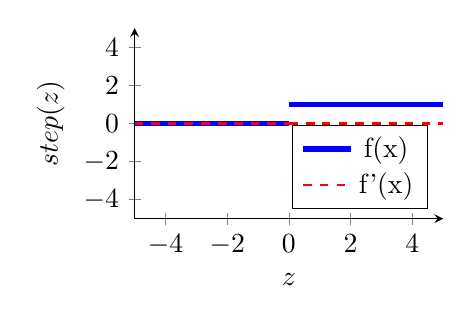
\begin{tikzpicture}
            \label{fig:threshold}
            \begin{axis}
                [width=5.5cm,height=4cm,ylabel=$step(z)$,xlabel=$z$,ymin=-5.0,ymax=5.0,xmin=-5,xmax=5,
                legend style={at={(0.95,0.05)},anchor=south east},]
                \addplot[blue,smooth, domain=-5:0] {0};
                \addplot[red,dashed, thick, domain=-5:0] {0};
                \addplot[blue,smooth, domain=-0:5] {1};
                \addplot[red,dashed, thick, domain=-0:5] {0};
                \addlegendentry{f(x)}
                \addlegendentry{f'(x)}
            \end{axis}
        \end{tikzpicture}
    }
    \subfloat[Linear]{
        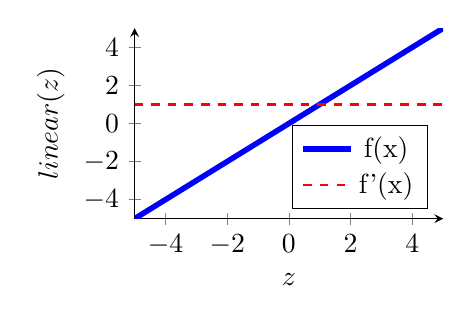
\begin{tikzpicture}
            \label{fig:linear}
            \begin{axis}
                [width=5.5cm,height=4cm,ylabel=$linear(z)$,xlabel=$z$,ymin=-5.0,ymax=5.0,xmin=-5,xmax=5,
                legend style={at={(0.95,0.05)},anchor=south east},]
                \addplot[blue,smooth] {x};
                \addlegendentry{f(x)}
                \addplot[red,dashed, thick] {1};
                \addlegendentry{f'(x)}
            \end{axis}
        \end{tikzpicture}
    }
    \subfloat[Sigmoid]{
        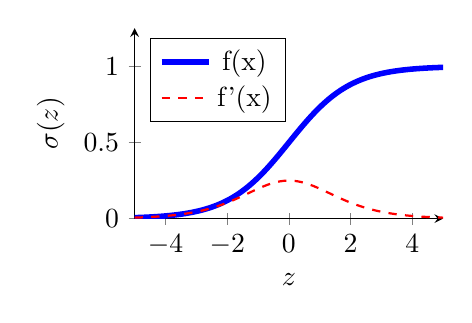
\begin{tikzpicture}
            \label{fig:sigmoid}
            \begin{axis}
                [width=5.5cm,height=4cm,ylabel=$\sigma(z)$,xlabel=$z$,ymin=0,ymax=1.25,xmin=-5,xmax=5,
                legend style={at={(0.05,0.95)},anchor=north west},]
                \addplot[blue,smooth] {1/(1+exp(-x))};
                \addlegendentry{f(x)}
                \addplot[red, dashed, thick] {1/(1+exp(-x)) * (1-1/(1+exp(-x)))};
                \addlegendentry{f'(x)}
            \end{axis}
        \end{tikzpicture}
    }\\
    \subfloat[Hyperbolic tangent]{
        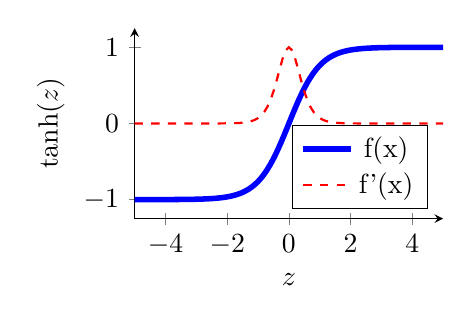
\begin{tikzpicture}
            \label{fig:hyperbolic_tangent}
            \begin{axis}
                [width=5.5cm,height=4cm,ylabel=$\tanh(z)$,xlabel=$z$,ymin=-1.25,ymax=1.25,xmin=-5,xmax=5, legend style={at={(0.95,0.05)},anchor=south east},]
                \addplot[blue,smooth] {tanh(x)};
                \addlegendentry{f(x)}
                \addplot[red,dashed, thick] {1/cosh(2*x)*1/cosh(2*x)};
                \addlegendentry{f'(x)}
            \end{axis}
        \end{tikzpicture}
    }
    \subfloat[ReLU]{
        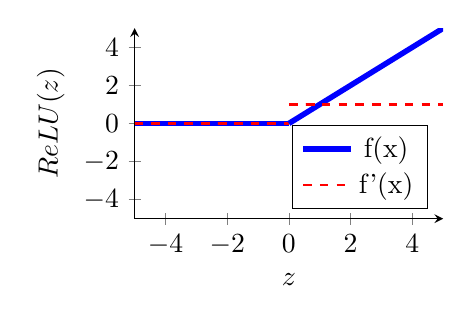
\begin{tikzpicture}
            \label{fig:relu}
            \begin{axis}
                [width=5.5cm,height=4cm,ylabel=$ReLU(z)$,xlabel=$z$,ymin=-5.0,ymax=5.0,xmin=-5,xmax=5,
                legend style={at={(0.95,0.05)},anchor=south east},]
                \addplot[blue,smooth, domain=-5:0] {0};
                \addplot[red,dashed, thick, domain=-5:0] {0};
                \addplot[blue,smooth, domain=-0:5] {x};
                \addplot[red,dashed, thick, domain=-0:5] {1};
                \addlegendentry{f(x)}
                \addlegendentry{f'(x)}
            \end{axis}
        \end{tikzpicture}
    }
    \subfloat[Leaky ReLU]{
        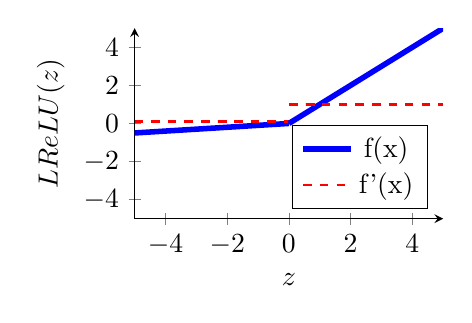
\begin{tikzpicture}
            \label{fig:lrelu}
            \begin{axis}
                [width=5.5cm,height=4cm,ylabel=$LReLU(z)$,xlabel=$z$,ymin=-5.0,ymax=5.0,xmin=-5,xmax=5,
                legend style={at={(0.95,0.05)},anchor=south east},]
                \addplot[blue,smooth, domain=-5:0] {0.1*x};
                \addplot[red,dashed, thick, domain=-5:0] {0.1};
                \addplot[blue,smooth, domain=-0:5] {x};
                \addplot[red,dashed, thick, domain=-0:5] {1};
                \addlegendentry{f(x)}
                \addlegendentry{f'(x)}
            \end{axis}
        \end{tikzpicture}
    }\\
    \subfloat[GELU]{
        \begin{tikzpicture}
            \label{fig:gelu}
            \begin{axis}
                [width=5.5cm,height=4cm,ylabel=$GELU(z)$,xlabel=$z$,ymin=-5.0,ymax=5.0,xmin=-5,xmax=5,
                legend style={at={(0.95,0.05)},anchor=south east},]
                \addplot[blue,smooth] {x * 0.5 * (1 + erf(x /sqrt(2)))};
                \addplot[red,dashed, thick] {0.5 * (1 + erf(x /sqrt(2))) + 1/sqrt(2*pi) * (exp(-x*x/2))};
                \addlegendentry{f(x)}
                \addlegendentry{f'(x)}
            \end{axis}
        \end{tikzpicture}
    }
    \subfloat[Swish]{
        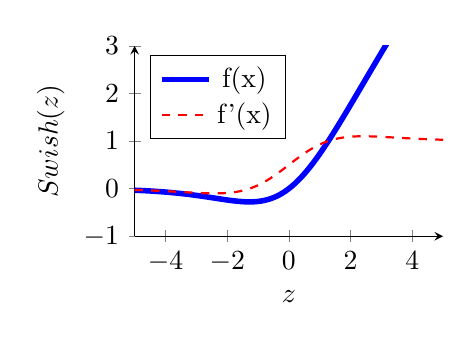
\begin{tikzpicture}
            \label{fig:swish}
            \begin{axis}
                [width=5.5cm,height=4cm,ylabel=$Swish(z)$,xlabel=$z$,ymin=-1,ymax=3.0,xmin=-5,xmax=5,
                legend style={at={(0.05,0.95)},anchor=north west},]
                \addplot[blue,smooth] {x*(1/(1+exp(-x)))}; % f (x) + σ (x) (1 − f (x))
                \addlegendentry{f(x)}
                \addplot[red, dashed, thick] {x/(1+exp(-x)) + 1/(1+exp(-x)) * (1-x/(1+exp(-x)))};
                \addlegendentry{f'(x)}
            \end{axis}
        \end{tikzpicture}
    }
    \subfloat[SIREN]{
        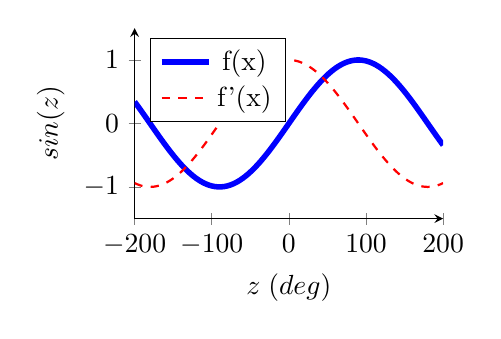
\begin{tikzpicture}
            \label{fig:siren}
            \begin{axis}
                [width=5.5cm,height=4cm,ylabel=$sin(z)$,xlabel=$z\;\text{(deg)}$,ymin=-1.5,ymax=1.5,xmin=-200,xmax=200,
                legend style={at={(0.05,0.95)},anchor=north west},]
                \addplot[blue,smooth,domain=-200:200] {sin(x)}; % f (x) + σ (x) (1 − f (x))
                \addlegendentry{f(x)}
                \addplot[red, dashed, thick,domain=-200:200] {cos(x)};
                \addlegendentry{f'(x)}
            \end{axis}
        \end{tikzpicture}
    }
    \caption[Activation functions.]{\textbf{Activation functions} used in \gls{DL}, included for results in their performance or historic significance in the applications of artificial neural networks.}
    \label{fig:activation-functions}
\end{figure}
%    \caption{Activation functions}
%    \label{fig:activation}
%\end{figure}
\makeatletter
\pgfmathdeclarefunction{erf}{1}{%
    \begingroup
    \pgfmathparse{#1 > 0 ? 1 : -1}%
    \edef\sign{\pgfmathresult}%
    \pgfmathparse{abs(#1)}%
    \edef\x{\pgfmathresult}%
    \pgfmathparse{1/(1+0.3275911*\x)}%
    \edef\t{\pgfmathresult}%
    \pgfmathparse{%
        1 - (((((1.061405429*\t -1.453152027)*\t) + 1.421413741)*\t
        -0.284496736)*\t + 0.254829592)*\t*exp(-(\x*\x))}%
    \edef\y{\pgfmathresult}%
    \pgfmathparse{(\sign)*\y}%
    \pgfmath@smuggleone\pgfmathresult%
    \endgroup
}
%dep
%subfig
\begin{figure}[htp]
    \centering
    \captionsetup{format=hang} % hanging captions
    \subfloat[Threshold Step]{
        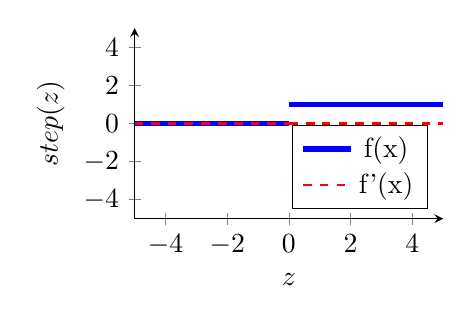
\begin{tikzpicture}
            \label{fig:threshold}
            \begin{axis}
                [width=5.5cm,height=4cm,ylabel=$step(z)$,xlabel=$z$,ymin=-5.0,ymax=5.0,xmin=-5,xmax=5,
                legend style={at={(0.95,0.05)},anchor=south east},]
                \addplot[blue,smooth, domain=-5:0] {0};
                \addplot[red,dashed, thick, domain=-5:0] {0};
                \addplot[blue,smooth, domain=-0:5] {1};
                \addplot[red,dashed, thick, domain=-0:5] {0};
                \addlegendentry{f(x)}
                \addlegendentry{f'(x)}
            \end{axis}
        \end{tikzpicture}
    }
    \subfloat[Linear]{
        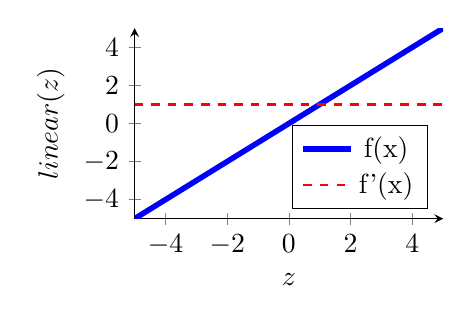
\begin{tikzpicture}
            \label{fig:linear}
            \begin{axis}
                [width=5.5cm,height=4cm,ylabel=$linear(z)$,xlabel=$z$,ymin=-5.0,ymax=5.0,xmin=-5,xmax=5,
                legend style={at={(0.95,0.05)},anchor=south east},]
                \addplot[blue,smooth] {x};
                \addlegendentry{f(x)}
                \addplot[red,dashed, thick] {1};
                \addlegendentry{f'(x)}
            \end{axis}
        \end{tikzpicture}
    }
    \subfloat[Sigmoid]{
        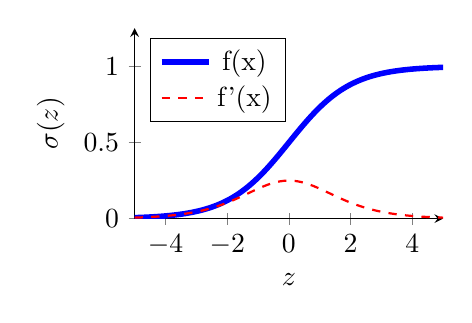
\begin{tikzpicture}
            \label{fig:sigmoid}
            \begin{axis}
                [width=5.5cm,height=4cm,ylabel=$\sigma(z)$,xlabel=$z$,ymin=0,ymax=1.25,xmin=-5,xmax=5,
                legend style={at={(0.05,0.95)},anchor=north west},]
                \addplot[blue,smooth] {1/(1+exp(-x))};
                \addlegendentry{f(x)}
                \addplot[red, dashed, thick] {1/(1+exp(-x)) * (1-1/(1+exp(-x)))};
                \addlegendentry{f'(x)}
            \end{axis}
        \end{tikzpicture}
    }\\
    \subfloat[Hyperbolic tangent]{
        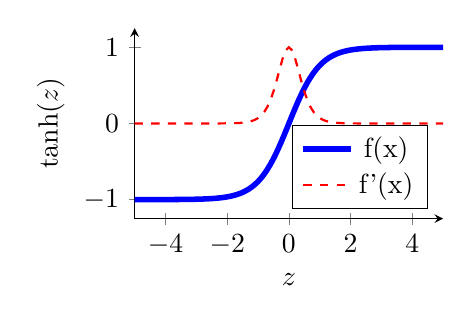
\begin{tikzpicture}
            \label{fig:hyperbolic_tangent}
            \begin{axis}
                [width=5.5cm,height=4cm,ylabel=$\tanh(z)$,xlabel=$z$,ymin=-1.25,ymax=1.25,xmin=-5,xmax=5, legend style={at={(0.95,0.05)},anchor=south east},]
                \addplot[blue,smooth] {tanh(x)};
                \addlegendentry{f(x)}
                \addplot[red,dashed, thick] {1/cosh(2*x)*1/cosh(2*x)};
                \addlegendentry{f'(x)}
            \end{axis}
        \end{tikzpicture}
    }
    \subfloat[ReLU]{
        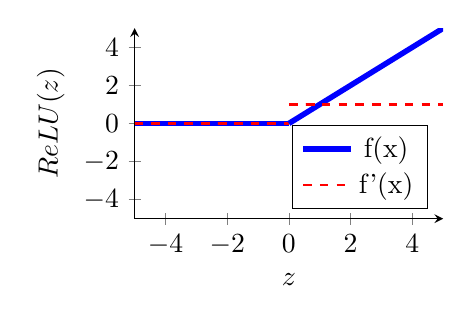
\begin{tikzpicture}
            \label{fig:relu}
            \begin{axis}
                [width=5.5cm,height=4cm,ylabel=$ReLU(z)$,xlabel=$z$,ymin=-5.0,ymax=5.0,xmin=-5,xmax=5,
                legend style={at={(0.95,0.05)},anchor=south east},]
                \addplot[blue,smooth, domain=-5:0] {0};
                \addplot[red,dashed, thick, domain=-5:0] {0};
                \addplot[blue,smooth, domain=-0:5] {x};
                \addplot[red,dashed, thick, domain=-0:5] {1};
                \addlegendentry{f(x)}
                \addlegendentry{f'(x)}
            \end{axis}
        \end{tikzpicture}
    }
    \subfloat[Leaky ReLU]{
        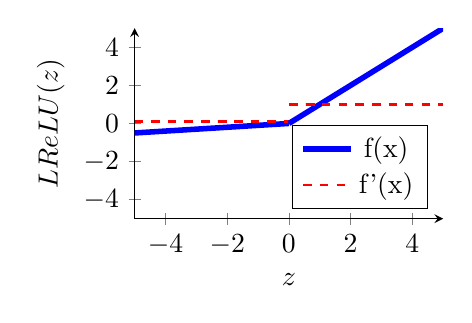
\begin{tikzpicture}
            \label{fig:lrelu}
            \begin{axis}
                [width=5.5cm,height=4cm,ylabel=$LReLU(z)$,xlabel=$z$,ymin=-5.0,ymax=5.0,xmin=-5,xmax=5,
                legend style={at={(0.95,0.05)},anchor=south east},]
                \addplot[blue,smooth, domain=-5:0] {0.1*x};
                \addplot[red,dashed, thick, domain=-5:0] {0.1};
                \addplot[blue,smooth, domain=-0:5] {x};
                \addplot[red,dashed, thick, domain=-0:5] {1};
                \addlegendentry{f(x)}
                \addlegendentry{f'(x)}
            \end{axis}
        \end{tikzpicture}
    }\\
    \subfloat[GELU]{
        \begin{tikzpicture}
            \label{fig:gelu}
            \begin{axis}
                [width=5.5cm,height=4cm,ylabel=$GELU(z)$,xlabel=$z$,ymin=-5.0,ymax=5.0,xmin=-5,xmax=5,
                legend style={at={(0.95,0.05)},anchor=south east},]
                \addplot[blue,smooth] {x * 0.5 * (1 + erf(x /sqrt(2)))};
                \addplot[red,dashed, thick] {0.5 * (1 + erf(x /sqrt(2))) + 1/sqrt(2*pi) * (exp(-x*x/2))};
                \addlegendentry{f(x)}
                \addlegendentry{f'(x)}
            \end{axis}
        \end{tikzpicture}
    }
    \subfloat[Swish]{
        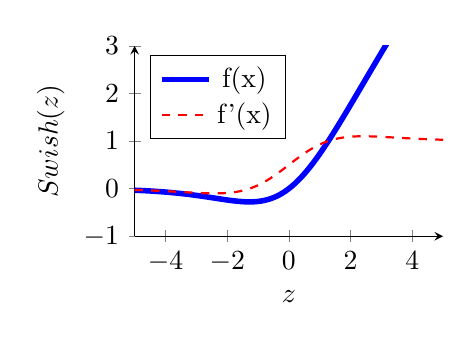
\begin{tikzpicture}
            \label{fig:swish}
            \begin{axis}
                [width=5.5cm,height=4cm,ylabel=$Swish(z)$,xlabel=$z$,ymin=-1,ymax=3.0,xmin=-5,xmax=5,
                legend style={at={(0.05,0.95)},anchor=north west},]
                \addplot[blue,smooth] {x*(1/(1+exp(-x)))}; % f (x) + σ (x) (1 − f (x))
                \addlegendentry{f(x)}
                \addplot[red, dashed, thick] {x/(1+exp(-x)) + 1/(1+exp(-x)) * (1-x/(1+exp(-x)))};
                \addlegendentry{f'(x)}
            \end{axis}
        \end{tikzpicture}
    }
    \subfloat[SIREN]{
        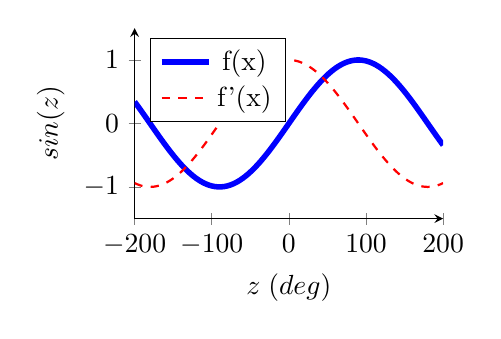
\begin{tikzpicture}
            \label{fig:siren}
            \begin{axis}
                [width=5.5cm,height=4cm,ylabel=$sin(z)$,xlabel=$z\;\text{(deg)}$,ymin=-1.5,ymax=1.5,xmin=-200,xmax=200,
                legend style={at={(0.05,0.95)},anchor=north west},]
                \addplot[blue,smooth,domain=-200:200] {sin(x)}; % f (x) + σ (x) (1 − f (x))
                \addlegendentry{f(x)}
                \addplot[red, dashed, thick,domain=-200:200] {cos(x)};
                \addlegendentry{f'(x)}
            \end{axis}
        \end{tikzpicture}
    }
    \caption[Activation functions.]{\textbf{Activation functions} used in \gls{DL}, included for results in their performance or historic significance in the applications of artificial neural networks.}
    \label{fig:activation-functions}
\end{figure}
%
\newpage

\subsection{Optimization of Neural Networks}
%%%%%%%%%%%%%%%%%%%%%%%%%%%%%%%%%%%%%%%%%%%%%%%%%%%%%%%%%%%%%%%%%%%%%%%%%%%%%%%%


It was seen in \autoref{eq:} that the partial differential of \gls{ml:J} can be
expressed with respect to the model parameters of a \gls{MLP}. These first
order expressions can therefore be used in gradient optimization of the network.
This is referred to as \textbf{gradient descent}, of which there are three
variants which differ in their use of the training dataset.

\begin{itemize}
    \item \textbf{\Gls{GD}}, a.k.a. batch gradient descent or vanilla gradient
    descent computes the gradient of the cost function over the entire training
    dataset and performs a single update:
    \begin{equation}
        \gls{dl:theta}_{t+1} = \gls{dl:theta}_t - \gls{dl:lr} \nabla_{\gls{dl:theta}}\gls{dl:J}(\gls{dl:theta}_t)
        \label{eq:dl:opt:gd}
    \end{equation}
    This method of gradient descent can be slow and intractable for datasets
    that do not fit in memory. This method of optimization is also incompatible
    with \textit{online} learning. \cite{ruder2017overview}

    \item \textbf{\Gls{SGD}} computes the gradient of the cost function for
    \textit{each} example in the dataset and performs an update for each
    input-output pair in the dataset:
    \begin{equation}
        \gls{dl:theta}_{t+1} = \gls{dl:theta}_t - \gls{dl:lr} \nabla_{\gls{dl:theta}}\gls{dl:J}(\gls{dl:theta}_t;\gls{ml:x:i},\gls{ml:y_true:i})
        \label{eq:dl:opt:sgd}
    \end{equation}
    Batch gradient descent often results in redundant gradient calculations for
    large datasets when encountering similar examples. \Gls{SGD} overcomes this
    redundancy however exhibits updates with high variance which can cause high
    fluctuations in the cost function. These high fluctuations result in
    overshooting of the minima being converged towards, and therefore often
    requires a lower learning rate than \Gls{GD}. \cite{ruder2017overview}

    \item \textbf{\Gls{MB-SGD}} has the advantages of both \gls{SGD} and \gls{GD},
    computing the gradient of the cost function for every mini-batch of \gls{ml:m}
    training examples:
    \begin{equation}
        \gls{dl:theta}_{t+1} = \gls{dl:theta}_t - \gls{dl:lr} \nabla_{\gls{dl:theta}}\gls{dl:J}(\gls{dl:theta}_t;\gls{ml:x:i:i+m},\gls{ml:y_true:i:i+m})
        \label{eq:dl:opt:mb_sgd}
    \end{equation}
    Memory constraints are no longer encountered (as in \Gls{GD}), and high
    variance in updates are avoided (as in \Gls{SGD}). Mini-batch gradient
    descent methods are the typical choice when training a neural architecture
    \cite{ruder2017overview}. \textbf{Note} that the term \Gls{SGD} is very
    often used in literature to refer to \Gls{MB-SGD}.

\end{itemize}

Some challenges exist for vanilla gradient descent methods, most of which
concern the topology of the cost function. Constant learning rates can lead to
slow convergence, especially when a saddle point in encountered in the cost
function in non-convex problems, which are notoriously difficult to escape. This
motivates the need to schedule, adapt or augment the learning rate throughout
the learning process. This issues are addressed by the specific variants of the
optimization algorithms used. For the next section, the parameters in the
notation $\nabla_{\gls{dl:theta}}\gls{dl:J}(\gls{dl:theta}_k; \ldots)$ are
dropped, as it is implicitly defined by the choice of batch size in \Gls{MB-SGD}
(as mentioned, a.k.a. \gls{SGD}).

\begin{figure}[htp]
    %%%%%%%%%%%%%%%%%%%%%%%%%%%%%%%%%%%%%%%%%%%%%%%%%%%%%%%%%%%%%%%%%%%%%%%%%%%%%%%%%%%
    \begin{subfigure}[b]{0.49\textwidth}
        \centering
        \begin{tikzpicture}
    \begin{axis}
        [samples=20,
        ylabel=$\theta_2$,
        xlabel=$\theta_1$,
        zlabel=$\gls{ml:J}(\gls{dl:theta})$,
        ticks=none,
        xticklabels={\empty},
        yticklabels={\empty},
        ]
        \addplot3[
        surf,
        domain y=0:15,
        domain=-3.141:3.141,
        ] {-125*(cos(deg(x)))+y^2};
        \addplot3[color=black,mark=o] table[col sep=comma] {code/output/vanilla_lr0.015.csv};
    \end{axis}
\end{tikzpicture}
        \subcaption{Slow learning rate (Low $\gls{dl:lr}$)}
        \label{fig:gd-low-eta}
    \end{subfigure}\hfil
    %%%%%%%%%%%%%%%%%%%%%%%%%%%%%%%%%%%%%%%%%%%%%%%%%%%%%%%%%%%%%%%%%%%%%%%%%%%
    \begin{subfigure}[b]{0.49\textwidth}
        \centering
        \begin{tikzpicture}
    \begin{axis}
        [samples=20,
        ylabel=$\theta_2$,
        xlabel=$\theta_1$,
        zlabel=$\gls{ml:J}(\gls{dl:theta})$,
        ticks=none,
        xticklabels={\empty},
        yticklabels={\empty},]
        \addplot3[
        surf,
        domain y=0:15,
        domain=-3.141:3.141,
        ] {-125*(cos(deg(x)))+y^2};
        \addplot3[color=black,mark=o] table[col sep=comma] {code/output/vanilla_lr0.025.csv};
    \end{axis}
\end{tikzpicture}

        \subcaption{Medium learning rate (Medium $\gls{dl:lr}$)}
        \label{fig:gd-medium-eta}
    \end{subfigure}\hfil
    %%%%%%%%%%%%%%%%%%%%%%%%%%%%%%%%%%%%%%%%%%%%%%%%%%%%%%%%%%%%%%%%%%%%%%%%%%%%%%%%%%%
    \captionsetup{format=hang} % hanging captions
    \caption{
        An illustration of \gls{SGD} at varied levels of learning rate
        (\gls{dl:lr}), in the convergence of the cost function optimization
        (\gls{ml:J}) with a ravine-like topology. \gls{SGD} notoriously has
        trouble navigating ravines, seen by its oscillation across the slops of
        the ravine, with hesitant progress towards the minima. a) shows a very
        slow convergence with a constant low setting of $\gls{dl:lr}$. b) shows
        an overshooting of the ravine's trough with a constant medium setting of
        \gls{dl:lr}. There exists a third case where \gls{dl:lr} is set to an
        excessive value, causing the first update to exit the ravine-like
        topology entirely.
    }
    \label{fig:vanilla-gd-learning}
\end{figure}

\subsubsection{Gradient descent optimization algorithms}
%\hline

\textbf{Momentum}~\cite{QIAN1999145} was introduced to deal with the problem
that \gls{SGD} exhibits in ravine-like topology
(\autoref{fig:vanilla-gd-learning}), accelerating the descent along the relevant
direction, while dampening it in the other direction~\cite{ruder2017overview}.
This technique is often compared to that of a ball rolling down a ravine, with
momentum building up in the relevant direction.
This is achieved through adding a fraction ($\gamma$) of the previous update to
the current update:
\begin{equation}
    \begin{aligned}
        \bm{v}_t                  &= \gamma{}\bm{v}_{t-1} + \gls{dl:lr} \nabla_{\gls{dl:theta}}\gls{dl:J}(\gls{dl:theta}_t) \\
        \gls{dl:theta}_{t+1} &= \gls{dl:theta}_t - \bm{v}_t
        \label{eq:dl:opt:sgd_momentum}
    \end{aligned}
\end{equation}

\textbf{\Gls{NAG}}~\cite{Nesterov1983AMF} addresses a shortcoming of momentum.
This technique adds a mechanism which can be compared to a \textit{smarter} ball
rolling down the hill, which slows down before the hill slopes up again after
the lowest point. This is achieved through the use of the momentum term $\gamma
\bm{v}_{t-1}$, although the gradient of cost function is evaluated at
$\gls{dl:theta}_t-\gamma \bm{v}_{t-1}$, a rough guess where the parameters are going
to be, rather than $\gls{dl:theta}_t$:
\begin{equation}
    \begin{aligned}
        \bm{v}_t &= \gamma \bm{v}_{t-1} + \gls{dl:lr} \nabla_{\gls{dl:theta}}\gls{dl:J}(\gls{dl:theta}_k - \gamma \bm{v}_{t-1}) \\
        \gls{dl:theta}_{t+1} &= \gls{dl:theta}_t - \bm{v}_t
    \end{aligned}
\end{equation}

\textbf{Adagrad} \cite{JMLR:v12:duchi11a} adapts the learning rate
according to the historical updates of the parameters. Larger updates are
carried out for infrequently updated parameters, and smaller for those more
frequently updated. This property makes this algorithm perform well for sparsely
distributed data. The following is often set for simplicity in literature:
\begin{equation}
    g_{t,i} & = \nabla_{\gls{dl:theta}_i} \gls{dl:J}(\gls{dl:theta}_k)
\end{equation}
Adagrad modifies the learning rate $\eta$ at each time step $t$ using the
past computed gradients for each parameter $\theta_i$ as:
\begin{equation}
    \gls{dl:theta}_{t+1,i} &= \gls{dl:theta}_{t,i} -\frac{\gls{dl:lr}}{\sqrt{G_{t,ii}+\epsilon}}\cdot{g_{t,i}}
\end{equation}
Where $G_t$ is a diagonal matrix where each element $i,i$ corresponds to the sum
of the squares of all historical gradients of $g_i$, expressed by:
\begin{equation}
    G_t & = \sum_{t=1}^T \bm{g}_{\tau}^2
\end{equation}
A smoothing factor $\epsilon$ is used to avoid division by zero, typically set
as $1e-8$. The primary benefit of Adagrad is the elimination of the need to
manually tune $\gls{dl:lr}$, its is typically set and left at
$0.01$~\cite{ruder2017overview}. The primary weakness of Adagrad is that the
accumulated sum of squares of the gradient continuously grows during training,
causing the learning rate to asymptotically approach zero.

\textbf{Adadelta}~\cite{zeiler2012adadelta} is an extension of Adagrad
which aims to reduce its aggressive, monotomically decreasing learning rate.
Adadelta achieves this by storing a running average of the squared gradient
updates within a window, defined by a fraction $\gamma$ (similar to that seen in
momentum):
\begin{equation}
    \gls{E} [g^2]_t = \gamma{}\gls{E} [g^2]_{t-1} + (1-\gamma) g_t^2
\end{equation}
The fraction $\gamma$ is typically set at $0.9$ giving an effective window width
of 10 for the running average. The original authors introduce a second exponentially
decaying average, the running average of the squared gradient updates:
\begin{equation}
    \gls{E} [\Delta{\theta}^2]_t = \gamma{}\gls{E} [\Delta{\theta}^2]_{t-1} +
    (1-\gamma)\Delta{\theta}^2_{t}
\end{equation}b
From these expectations, the author approximates the RMS of the gradients and
parameter updates as:
\begin{equation}
    \begin{aligned}
        \text{RMS}[g]              & = \sqrt{\gls{E} [g^2] + \epsilon} \\
        \text{RMS}[\Delta{\theta}] & = \sqrt{\gls{E} [\Delta{\theta}^2] + \epsilon} \\
    \end{aligned}
\end{equation}
From which the final expression for the parameter updates are expressed:
\begin{equation}
    \begin{aligned}
        \Delta{\gls{dl:theta}_t} &= - \frac{\text{RMS}[\Delta{\gls{dl:theta}}]_{t-1}}{\text{RMS}[\bm{g}]_t}\cdot{}\bm{g}_t \\
        \gls{dl:theta}_{t+1} &= \gls{dl:theta}_t + \Delta{\gls{dl:theta}_t}
    \end{aligned}
\end{equation}
The motivation and derivation of the implementation are omitted here but can be
found in literature \cite{zeiler2012adadelta,ruder2017overview}. The key
takeaway is that there is no need to set the learning rate $\gls{dl:lr}$ to a
fixed value. \textcolor{red}{(Include personal experience on initial expectation
of parameter update?)}.

\textbf{RMSProp}~\cite{JMLR:v12:duchi11a}

\begin{equation}
    \begin{aligned}
        \gls{E} [\Delta{\theta}^2] &= \gamma{}\gls{E} [\Delta{\theta}^2]_{t-1} + (1-\gamma)\Delta{\theta}^2_{t} \\
        \gls{dl:theta}_{t+1}       &= \gls{dl:theta}_t + \frac{\gls{dl:lr}}{\sqrt{\gls{E} [\Delta{\theta}^2]_t+\epsilon}}\bm{g}_t
    \end{aligned}
\end{equation}

\textbf{Adam}~\cite{JMLR:v12:duchi11a}

\begin{equation}
    \begin{aligned}
        m_t &= \beta_1 m_{t-1} + (1-\beta_1)\bm{g}_t \\
        v_t &= \beta_2 v_{t-1} + (1-\beta_2)\bm{g}_t^2 \\
    \end{aligned}
\end{equation}

\begin{equation}
    \begin{aligned}
        \hat{m}_t &= \frac{m_t}{1-\beta_1^t} \\
        \hat{v}_t &= \frac{v_t}{1-\beta_2^t} \\
    \end{aligned}
\end{equation}

\begin{equation}
    \begin{aligned}
        \Delta{\gls{dl:theta}_t} &= - \frac{\hat{m}_t}{\sqrt{\hat{v}_t} + \epsilon} \bm{g}_t \\
        \gls{dl:theta}_{t+1}       &= \gls{dl:theta}_t + \Delta{\gls{dl:theta}_t}
    \end{aligned}
\end{equation}

\begin{figure}[htp]
    \centering
    %! Author = ggarr
%! Date = 05/01/2022

\begin{tikzpicture}
    \begin{axis}
        [samples=20,
        ylabel=$\theta_2$,
        xlabel=$\theta_1$,
        zlabel=$\gls{ml:J}(\gls{dl:theta})$,
        ticks=none,
        xticklabels={\empty},
        yticklabels={\empty},
        ]
        \addplot3[
        surf,
        domain y=0:15,
        domain=-3.141:3.141,
        ] {-125*(cos(deg(x)))+y^2};
        \addplot3[color=black,mark=o] table[col sep=comma] {code/output/adam2.csv};
    \end{axis}
\end{tikzpicture}



    %%%%%%%%%%%%%%%%%%%%%%%%%%%%%%%%%%%%%%%%%%%%%%%%%%%%%%%%%%%%%%%%%%%%%%%%%%%%%%%%%%%
    \captionsetup{format=hang} % hanging captions
    \caption{
        Vanilla gradient descent methods with an illustration of the effect of
        varied levels of learning rate (\gls{dl:lr}), in the convergence of the
        cost function optimization (\gls{ml:J}) with a ravine-like topology. a)
        shows a very slow convergence with a constant low setting of
        $\gls{dl:lr}$. b) shows an overshooting of the minimum with a constant
        medium setting of \gls{dl:lr}. There exists a third case where
        \gls{dl:lr} is set to an excessive value, causing the first update to
        exit the ravine-like topology entirely.
    }
    \label{fig:vanilla-gd-learning}
\end{figure}
It should be noted that in addition to these, there are the popular
\textbf{AdaMax} and \textbf{Nadam} \cite{ruder2017overview} methods. The AdaMax
algorithm is a generalization of the Adam algorithm, which uses $\ell_2$ norms,
allowing formulation with any $\ell_p$ norm. The Nadam algorithm incorporates a
combination of the elements used in the \gls{NAG} and Adam algorithms. These
algorithms are not included here as their use is sparse throughout literature,
rather the RMSProp and Adam algorithms are most commonly used.
\textcolor{red}{More motivation here}




\item \textbf{\Gls{Learning to Optimize}}: \cite{ruder2017overview,Li2017}

%
%\subsection{Gradient based learning}
%%%%%%%%%%%%%%%%%%%%%%%%%%%%%%%%%%%%%%%%%%%%%%%%%%%%%%%%%%%%%%%%%%%%%%%%%%%%%%%%%
%

%
%\begin{equation}
%    \pardiff{\gls{ml:J}}{\gls{dl:w:l:jk}}
%    =
%    \pardiff{\gls{ml:J}}{\gls{dl:z:l:j}}
%    \pardiff{\gls{dl:z:l:j}}{\gls{dl:w:l:jk}}
%\end{equation}
%
%\begin{equation}
%    \gls{dl:z:l:j} = \sum_{k=1}^{\gls{dl:n:h:l}}\gls{dl:w:l:jk}\gls{dl:a:lm1:k}+\gls{dl:b:l:j}
%\end{equation}
%
%%\begin{equation}
%%    \frac{\partial{u^{(n)}}}{\partial{u^{(j)}}} = \sum_{\text{path($u^{(\pi_1)}, u^{(\pi_2)}, \ldots, u^{(\pi_t)}$), \\ from $\pi_1=j$ to $\pi_t=n$}}
%%\end{equation}
%
%Backpropagation, short for "backward propagation of errors," is a
%\textit{supervised learning} algorithm for artificial neural networks using
%\textit{gradient descent}.
%
%\begin{figure}[htp]
%    \centering
%    
% https://github.com/davidstutz/latex-resources/blob/master/tikz-gradient-descent/gradient-descent.tex
% \usepackage{tikz}
% \usepackage{tikz}
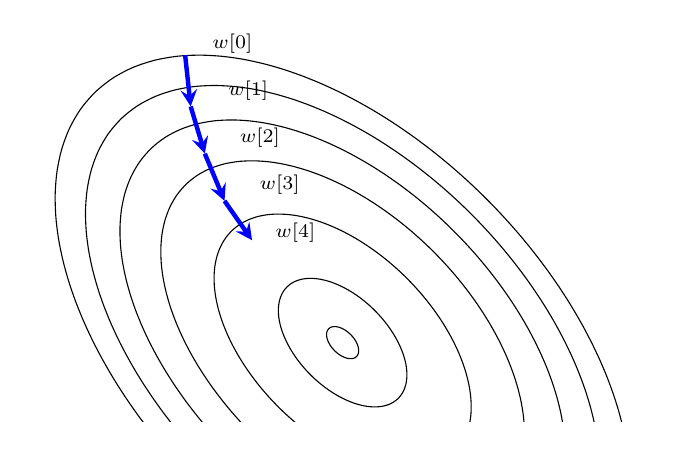
\begin{tikzpicture}[samples=100,smooth]
    \begin{scope}
        \clip(-4,-1) rectangle (4,4);
        \draw plot[domain=0:360] ({cos(\x)*sqrt(20/(sin(2*\x)+2))},{sin(\x)*sqrt(20/(sin(2*\x)+2))});
        \draw plot[domain=0:360] ({cos(\x)*sqrt(16/(sin(2*\x)+2))},{sin(\x)*sqrt(16/(sin(2*\x)+2))});
        \draw plot[domain=0:360] ({cos(\x)*sqrt(12/(sin(2*\x)+2))},{sin(\x)*sqrt(12/(sin(2*\x)+2))});
        \draw plot[domain=0:360] ({cos(\x)*sqrt(8/(sin(2*\x)+2))},{sin(\x)*sqrt(8/(sin(2*\x)+2))});
        \draw plot[domain=0:360] ({cos(\x)*sqrt(4/(sin(2*\x)+2))},{sin(\x)*sqrt(4/(sin(2*\x)+2))});
        \draw plot[domain=0:360] ({cos(\x)*sqrt(1/(sin(2*\x)+2))},{sin(\x)*sqrt(1/(sin(2*\x)+2))});
        \draw plot[domain=0:360] ({cos(\x)*sqrt(0.0625/(sin(2*\x)+2))},{sin(\x)*sqrt(0.0625/(sin(2*\x)+2))});

        \draw[->,blue,ultra thick] (-2,3.65) to (-1.93,3);
        \draw[->,blue,ultra thick] (-1.93,3) to (-1.75,2.4);
        \draw[->,blue,ultra thick] (-1.75,2.4) to (-1.5,1.8);
        \draw[->,blue,ultra thick] (-1.5,1.8) to (-1.15,1.3);

        \node at (-1.4,3.8){\scriptsize $w[0]$};
        \node at (-1.2,3.2){\scriptsize $w[1]$};
        \node at (-1.05,2.6){\scriptsize $w[2]$};
        \node at (-0.8,2){\scriptsize $w[3]$};
        \node at (-0.6,1.4){\scriptsize $w[4]$};
    \end{scope}
\end{tikzpicture}

%    \caption{Gradient based learning}
%    \label{fig:gradient-descent}
%\end{figure}
%
%
%\begin{figure}[htp]
%    \centering
%    

% \pgfplotsset{compat=1.17}
% \usetikzlibrary{decorations.pathreplacing}
% \usepackage{pgfplots}

\tikzset{arrowed/.style={decorate,

decoration={show path construction,
moveto code={},
lineto code={
    \draw[#1] (\tikzinputsegmentfirst) --  (\tikzinputsegmentlast);
},
curveto code={},
closepath code={},
}},arrowed/.default={-stealth}}
\pgfplotsset{gradient function/.initial=f,
    dx/.initial=0.01,dy/.initial=0.01}
\pgfmathdeclarefunction{xgrad}{2}{%
    \begingroup%
    \pgfkeys{/pgf/fpu,/pgf/fpu/output format=fixed}%
    \edef\myfun{\pgfkeysvalueof{/pgfplots/gradient function}}%
    \pgfmathparse{(\myfun(#1+\pgfkeysvalueof{/pgfplots/dx},#2)%
    -\myfun(#1,#2))/\pgfkeysvalueof{/pgfplots/dx}}%
    % \pgfmathsetmacro{\mysum}{\mysum+\myfun(\value{isum},#2)}%
    \pgfmathsmuggle\pgfmathresult\endgroup%
}%
\pgfmathdeclarefunction{ygrad}{2}{%
    \begingroup%
    \pgfkeys{/pgf/fpu,/pgf/fpu/output format=fixed}%
    \edef\myfun{\pgfkeysvalueof{/pgfplots/gradient function}}%
    \pgfmathparse{(\myfun(#1,#2+\pgfkeysvalueof{/pgfplots/dy})%
    -\myfun(#1,#2))/\pgfkeysvalueof{/pgfplots/dy}}%
    % \pgfmathsetmacro{\mysum}{\mysum+\myfun(\value{isum},#2)}%
    \pgfmathsmuggle\pgfmathresult\endgroup%
}%

\begin{tikzpicture}
    \begin{axis}
        [width=12cm,%
        declare function={f(\x,\y)=cos(deg(\x)*0.8)*cos(deg(\y)*0.6)*exp(0.1*\x);}]
        \addplot3[surf,shader=interp,domain=-4:4,%samples=81
        ]{f(x,y)};
        \edef\myx{0.15} % first x coordinate
        \edef\myy{-0.15} % first y coordinate
        \edef\mystep{-2}% negative values mean descending
        \pgfmathsetmacro{\myf}{f(\myx,\myy)}
        \edef\lstCoords{(\myx,\myy,\myf)}
        \pgfplotsforeachungrouped\X in{0,...,5}
            {
            \pgfmathsetmacro{\myx}{\myx+\mystep*xgrad(\myx,\myy)}
            \pgfmathsetmacro{\myy}{\myy+\mystep*ygrad(\myx,\myy)}
            \pgfmathsetmacro{\myf}{f(\myx,\myy)}
            \edef\lstCoords{\lstCoords\space (\myx,\myy,\myf)}
        }
        \addplot3[samples y=0,arrowed] coordinates \lstCoords;
    \end{axis}
\end{tikzpicture}
%    \caption{Gradient based learning}
%    \label{fig:gradient-descent}
%\end{figure}
%
%\subsection{Universal Approximation Properties and Depth}
%%%%%%%%%%%%%%%%%%%%%%%%%%%%%%%%%%%%%%%%%%%%%%%%%%%%%%%%%%%%%%%%%%%%%%%%%%%%%%%%%
%
%A linear model by definition, may only optimised to represent linear functions.
%It has advantages in its simplicity to optimise however we often require our
%estimator models to learn nonlinear functions.
%
%%\subsection{Backpropagation}
%%%%%%%%%%%%%%%%%%%%%%%%%%%%%%%%%%%%%%%%%%%%%%%%%%%%%%%%%%%%%%%%%%%%%%%%%%%%%%%%%
%
%
\subsection{Common Frameworks and Techniques}

\newpage\subsection{Deep Learning in Space Exploration}

Disregarding the disagreements of whether space should be privatised or remain
only in the public sector, the uncertain economic returns of space exploration
are well known to be a key hindrance to progress in the field. Space
exploration is expensive, and this uncertainty of return is unattractive to
profit-seeking companies, making stakeholders far and few between. As a result,
the most successful results from \gls{DL} are rarely used in space exploration
due to neural networks not being human readable~\cite{esa_ai}. Interpretation of
neural networks have come a far way however, but require a deep understanding
of the problem domain for effective understanding of the way in which the
network is approaching its given task~\cite{Montavon2018, Sheu2020,
goh2021multimodal, molnar_2022}. The tasks most interpretable tend to be those
that are relatable learning tasks to the human mind, such as language
understanding, vision, and speech recognition.

\gls{DL} in space exploration has been a hot topic of research in recent years,
some examples of the learning tasks have been toward autonomy in docking
\cite{}, navigation, and environment modelling~\cite{IzzoGeodesyNet2021,
IzzoBennu2021}. The former two are tasks coupled within a joint
\gls{DL}-\gls{RL} framework, which are covered in \autoref{chap:DL}. The results
of Izzo et al. in the latter task are particularly promising, as they have
demonstrated that artificial neural networks can be used accurate geodetic models
of highly irregular bodies given minimal prior information on the body. Their
novel method is referred to as using a geodesyNet, which is a neural network
that learns a three-dimensional, differentiable mapping of the body's density,
that the authors refer to as a neural density field~\cite{IzzoGeodesyNet2021}.
The authors use a modified \gls{MAE} loss function to train the network, which
allows the network to focus on learning the deviation from a homogeneously
filled volume $V$, and not concurrently the absolute value of the body mass.
This is achieved using the factor $\kappa$:

\begin{equation}
    \kappa = \frac{\sum^n_{i=1}\hat{y}_i{}y_i}{\sum^m_{i=1}y_i^2},
\end{equation}

which modifies the original \gls{MAE} (see \autoref{chap:ML}) loss function to
the following form:

\begin{equation}
    \gls{J}_{\kappa\text{MAE}} = \frac{1}{\gls{ml:m}}\sum_{i=1}^{\gls{ml:m}}||{y}^{(i)}-\kappa{}\hat{y}^{(i)}||_1.
    \label{eq:MAE}
\end{equation}

\begin{equation}

\begin{figure}
    \centering
    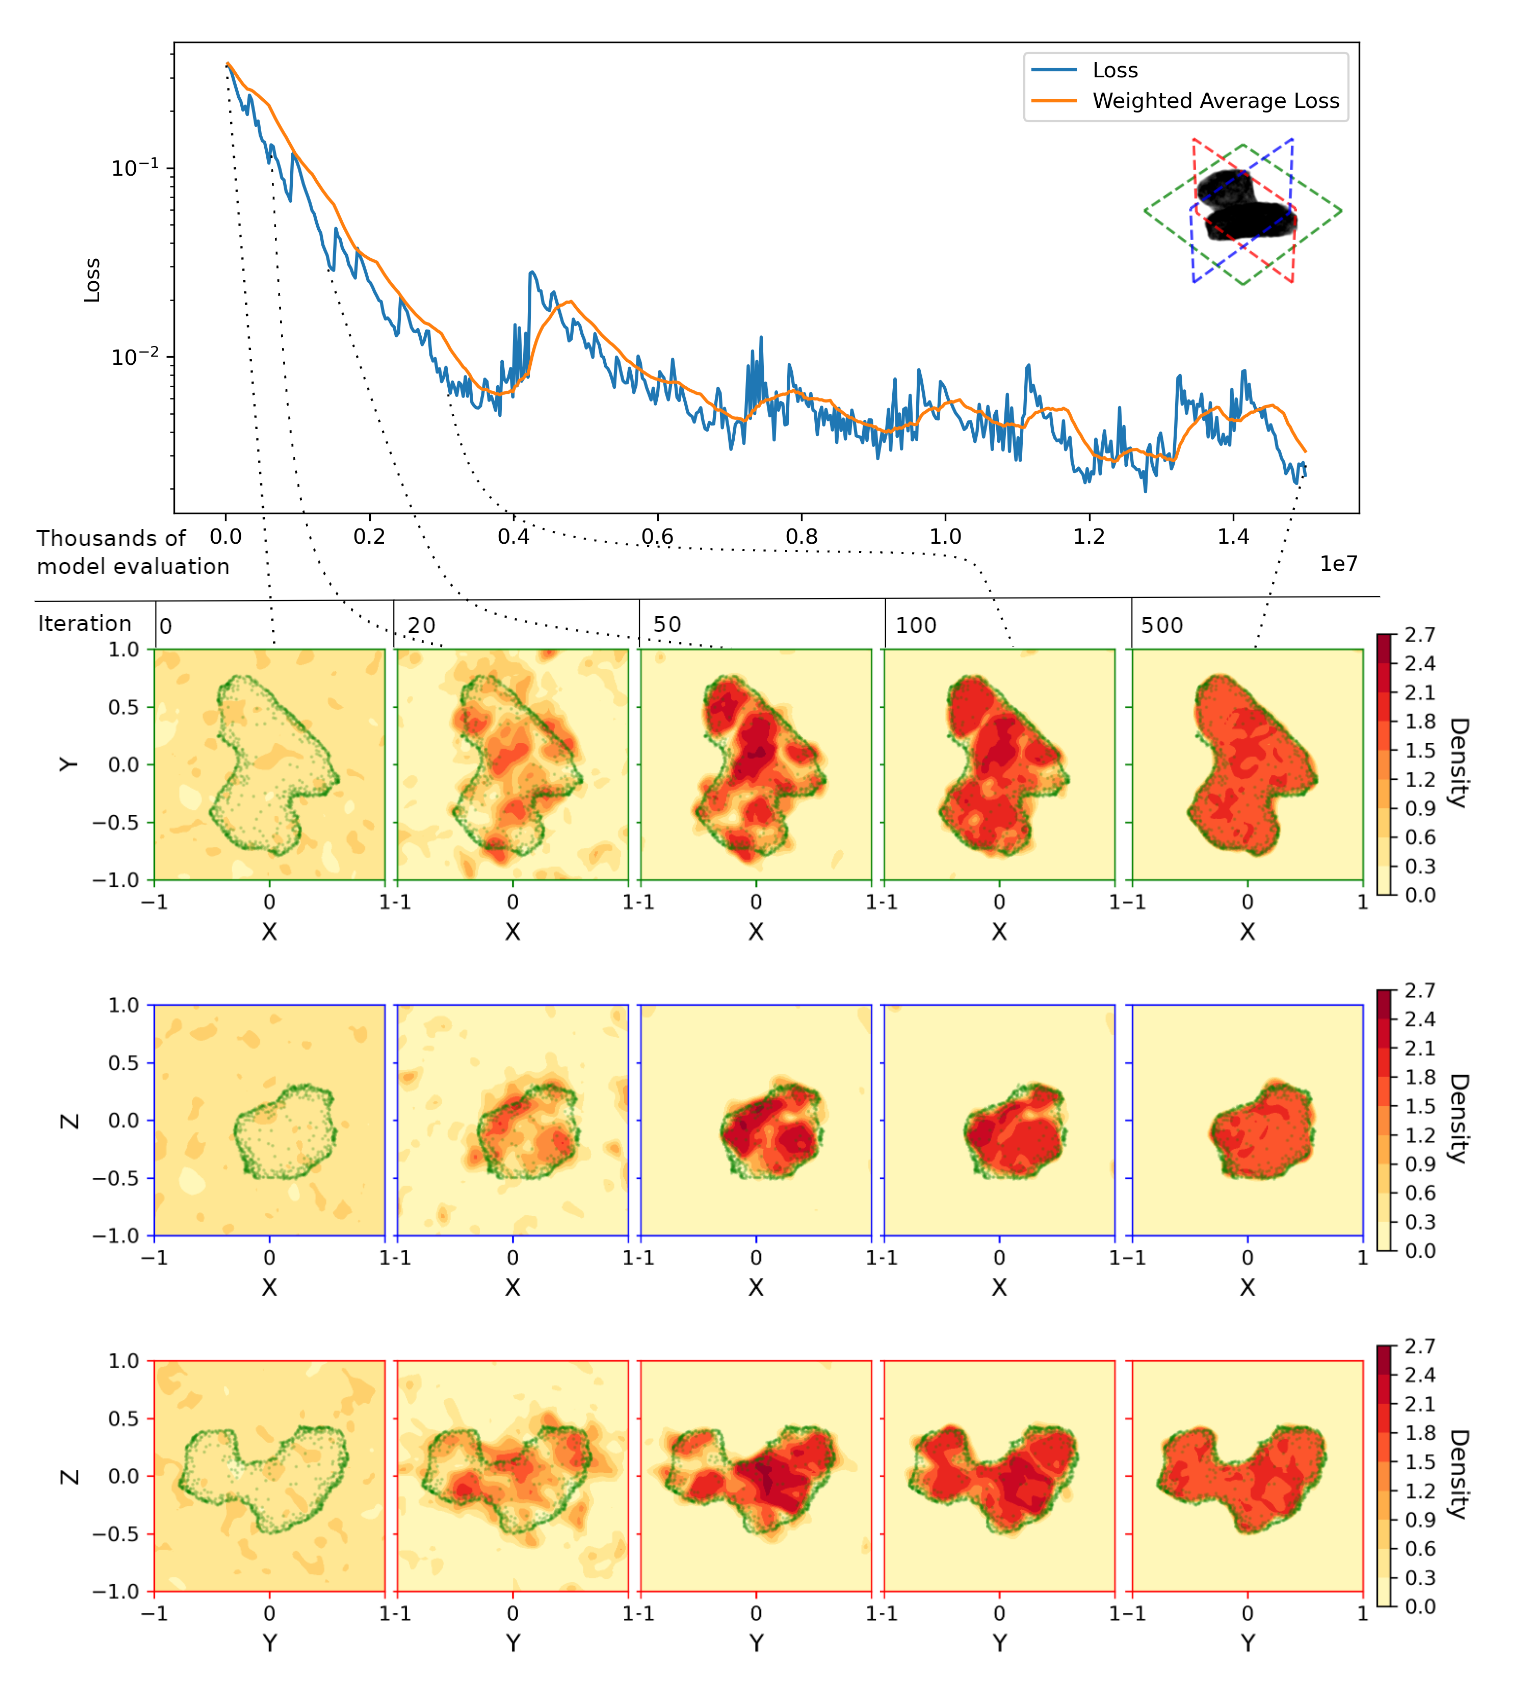
\includegraphics[width=0.8\linewidth]{graphics/geodesynet-example}
    \caption{GeodesyNet~\cite{IzzoGeodesyNet2021}}
    \label{fig:geodesy-net}
\end{figure}




\cite{Kothari2020}
%%%%%%%%%%%%%%%%%%%%%%%%%%%%%%%%%%%%%%%%%%%%%%%%%%%%%%%%%%%%%%%%%%%%%%%%%%%%%%%%

%\newpage\section{Reinforcement Learning}\label{sec:reinforcement_learning}
%%%%%%%%%%%%%%%%%%%%%%%%%%%%%%%%%%%%%%%%%%%%%%%%%%%%%%%%%%%%%%%%%%%%%%%%%%%%%%%%

Reinforcement learning is a type of machine learning that focuses on tasks in which an agent receives a reward (or penalty) signal at each time step throughout its engagement with an environment in which it lives in, and interacts with it through decisions on which action to take. The roots of this field go back to Dr. Richard Bellman in 1954, who is also known as the ``Father of Dynamic Programming''. His works on Dynamic Programming \cite{Bellman1954,Bellman1957a}

\tikzset{basic/.style={draw,text width=1em,text badly centered}}
\tikzset{component/.style={rectangle, draw=black, thick, text width=7em,align=center, rounded corners, minimum height=2em}}

\begin{figure}[!htp]
    \centering
    \captionsetup{format=hang} % hanging captions

    \tikzstyle{block} = [rectangle, draw,
    text width=8em, text centered, rounded corners, minimum height=4em]

    \tikzstyle{line} = [draw, -latex]

    \begin{tikzpicture}[node distance = 6em, auto, thick]
        \node [block] (Agent) {Agent};
        \node [block, below=5em of Agent] (Environment) {Environment};
        \node [left=3em of Environment] (Dashed) {};
        \node [above=1.7em of Dashed] (Dashed-up) {};
        \node [below=1.7em of Dashed] (Dashed-down) {};

        \path [line] (Agent.0) --++ (4em,0em) |- node [near start]{Action, $a_t$} (Environment.0);

        \path [line] (Environment.190) -- (Environment.190-|Dashed-down.east) node [midway, label={[xshift=-0.0em]center:$s_{t+1}$}] {\phantom{$s_{t+1}$}};
        \path [line] (Environment.170) -- (Environment.170-|Dashed-up.east) node [midway, above, label={[xshift=-0.0em]center:$r_{t+1}$}] {\phantom{$r_{t+1}$}};

        \path [line] (Environment.190|-Environment.190) --++ (-6em,0em) |- node [near start] {} node [near start, label={[xshift=-0.0em]center:State, $s_t$}] {\phantom{State, $s_t$}} (Agent.170);
        \path [line] (Environment.170|-Environment.170) --++ (-4.25em,0em) |- node [near start, right] {} node [near start, right, label={[xshift=-0.0em]center:Reward, $r_t$}] {\phantom{Reward, $r_t$}} (Agent.190);

        \draw[dotted] (Dashed-up.east) -- (Dashed-down.east);


    \end{tikzpicture}
    \caption{\textbf{The agent-environment interaction interface} illustrates the interaction between an agent and its environment. The agent takes an action $a_t$ and receives a reward $r_{t+1}$ and a new state $s_{t+1}$, subject to the environment's dynamics.}
    \label{fig:agent-environment}

\end{figure}


\subsection{Key Concepts and Terminology}\label{ssec:key_concepts_and_terminology}
%%%%%%%%%%%%%%%%%%%%%%%%%%%%%%%%%%%%%%%%%%%%%%%%%%%%%%%%%%%%%%%%%%%%%%%%%%%%%%%%
The key concepts and terms used in \gls{RL} are heavily influenced by the field of control theory
\begin{itemize}
    % States and Observations
    \item States \& Observations: A state \gls{rl:s} is a full description of the environment, wheras an observation \gls{rl:o} is partial description of the state. It is said that the environment is \textbf{fully observed} if the agent has access to \gls{rl:s}, and that the environment is \textbf{partially observed} if the agent may only act on \gls{rl:o}. Note that consistent use of notation in \gls{RL} appears to be a primary challenge faced by many researchers, symptomatic of the inconcise use of the term \gls{rl:s} in instances where \gls{rl:o} would be more appropriate.
    
    % Actions
    \item Actions: An action \gls{rl:a} is a description of the agent's action in the environment. The \textbf{action space} is the set of all valid actions in the environment. Some environments have \textbf{discrete action spaces} whereas others have \textbf{continuous action spaces}, which can influence the applicability of some \gls{RL} algorithms (see \autoref{ssec:algorithms}). For the latter, the action space is real, $\gls{rl:A}\in\gls{set:R}$.

    % Policies
    \item Policies: A policy is a rule which determines what action the agent decides to take in the environment. A policy can be \textbf{deterministic}, in which case it is denoted by $\gls{rl:a}[_t]=\gls{rl:mu}(\gls{rl:s}[_t])$, or \textbf{stochastic}, in which case it is denoted by $\gls{rl:a}[_t]\sim\gls{rl:pi}(\cdot|\gls{rl:s}[_t])$. Deterministic policies are straightforward, an example is an \gls{MLP} (see \autoref{ssec:mlps}). Stochastic policies are separated further into \textbf{categorical policies} (used in discrete action spaces) and \textbf{diagonal Gaussian policies} used in continuous action spaces. Categorical stocastic policy neural networks are trained in the same way as a classifier. For a neural network
    
    % Rewards and Returns
    \item Rewards \& Returns: A reward $\gls{rl:r}[_t]$ is a signal received by the agent at each time step \gls{rl:t}[t]. There are two variants of rewards, \textbf{discounted} and \textbf{undiscounted}. The \textbf{finite-horizon undiscounted} return is the sum of all rewards received in within a finite horizon T,
          \begin{equation}
              R(\tau)=\sum_{t=0}^{T} r_t.
          \end{equation}
    The \textbf{infinite-horizon discounted} return, is the sum of all rewards ever returned, with the difference that rewards are discounted by how far in the future they are obtained. The discount factor is $\gls{rl:discount}\in(0,1)$, giving the expression,
    \begin{equation}
        \gls{rl:R}(\gls{rl:tau})=\sum_{{\gls{rl:t}[t]}=0}^{\infty} \gls{rl:discount}^{\gls{rl:t}[t]} \gls{rl:r}_{\gls{rl:t}[t]}.
    \end{equation}
    The intuition of the latter equation is evident, as we wish to place more importance on the immediate rewards from the environment rather than the future rewards. In the case of an \textbf{infinite-horizon} environment this factor is mandatory, as without it, there would be no incentive for the agent to reach the objective state sooner rather than later, in an excessively large period of time. Mathematically the infinite-horizon sum of rewards may not converge to a finite value, without the use of the discount factor. 



    % While the line between these two formulations of return are quite stark in RL formalism, deep RL practice tends to blur the line a fair bit—for instance, we frequently set up algorithms to optimize the undiscounted return, but use discount factors in estimating value functions.
\end{itemize}

\begin{equation}
    \gls{rl:V}^{\gls{rl:pi}}(\gls{rl:s})
    =
    {\displaystyle \mathop{\mathbb{E}}_{\gls{rl:tau}\sim\gls{rl:pi}}}
    \lbrack R(\gls{rl:tau})~|~\gls{rl:s}[_0]=\gls{rl:s}\rbrack,
\end{equation}

\begin{equation}
    \gls{rl:Q}^{\gls{rl:pi}}(\gls{rl:s}, \gls{rl:a})
    =
    {\displaystyle \mathop{\mathbb{E}}_{\gls{rl:tau}\sim\gls{rl:pi}}}
    \lbrack R(\gls{rl:tau})~|~\gls{rl:s}[_0]=\gls{rl:s},~\gls{rl:a}[_0]=\gls{rl:a}\rbrack,
\end{equation}

\begin{equation}
    \gls{rl:V}^{*}(\gls{rl:s})
    =
    \max_{\gls{rl:pi}}{\displaystyle \mathop{\mathbb{E}}_{\gls{rl:tau}\sim\gls{rl:pi}}}
    \lbrack R(\gls{rl:tau})~|~\gls{rl:s}[_0]=\gls{rl:s}\rbrack,
\end{equation}



\subsection{Markov Decision Processes (MDP)}\label{ssec:mdp}
%%%%%%%%%%%%%%%%%%%%%%%%%%%%%%%%%%%%%%%%%%%%%%%%%%%%%%%%%%%%%%%%%%%%%%%%%%%%%%%%
A \gls{MDP} is a discrete-time stochastic process which defines a mathematical framework for decision making. This concept underpins the mathematical formulation of much of reinforcement learning \cite{Bellman1957a}. An \gls{MDP} is a 5-tuple of the form $\tupleft\gls{rl:S},\gls{rl:A},\gls{rl:P},\gls{rl:R},\gls{rl:rho0}\tupright$ where:

\begin{itemize}
    \item \gls{rl:S} is the set of all valid states,
    \item \gls{rl:A} is the set of all valid actions,
    \item \gls{rl:R} : $\gls{rl:S} \times \gls{rl:A} \times \gls{rl:S} \gls{fn:maps} \gls{set:R}$ is the reward function, with $r_t = \gls{rl:R}(\gls{rl:s}_{\gls{rl:t}}, \gls{rl:a}_{\gls{rl:t}}, \gls{rl:s}_{\gls{rl:t}[t]+1})$,
    \item \gls{rl:P} : $\gls{rl:S}  \times \gls{rl:A} \gls{fn:maps} \mathcal{P}(\gls{rl:S})$ is the transition probability function, with $P(\gls{rl:s}'|\gls{rl:s},\gls{rl:a})$ being the probability of transitioning into state $s'$ if you start
          in state $s$ and take action $a$,
    \item and $\rho_0$ is the starting state distribution.
\end{itemize}

\gls{MDP} refers to the system exhibiting the Markov Property, which is the memoryless property of a stochastic system. This means that the future evolution of the Markov process depnds only on the present state, and not on past history. In practice, this is seen as the decisions of the agent and values of the system to be a function of solely the current state. A prerequisite of the decisions and values being effective and informative, is that the state representation be informative. The standard \gls{RL} world model is a \gls{MDP}, however not all \gls{RL} algorithms strictly adhere to the \gls{MDP} formalism. Ocassionally the discount factor \gls{rl:discount} is included in the \gls{MDP} tuple but due to it being optional in the case of a finite-horizon \gls{MDP}, it is often omitted for generality. Consequently the \gls{MDP} may be found in literature as a 6-tuple of the form $\tupleft\gls{rl:S},\gls{rl:A},\gls{rl:P},\gls{rl:R},\gls{rl:rho0},\gls{rl:discount}\tupright$.

\subsection{Partially Observable Markov Decision Processes (POMDP)}\label{ssec:pomdp}
%%%%%%%%%%%%%%%%%%%%%%%%%%%%%%%%%%%%%%%%%%%%%%%%%%%%%%%%%%%%%%%%%%%%%%%%%%%%%%%%
\Glspl{POMDP} were first described by Karl Johan Åström (a control theorist) in 1965 \cite{Astrom1965} in his discussion of \glspl{MDP} with imperfect information. This alternative mathematical framework is powerful in planning problems in environments with partial observability of states due to its careful quantification of the non-deterministic effects in the agents interaction with the environment, a critical problem in robotics \cite{Kurniawati2021}. Following the augmentation of the 5-tuple describing an \gls{MDP} (\autoref{ssec:mdp}) with two additional terms, a \gls{POMDP} is a 7-tuple of the form $\tupleft\gls{rl:S},\gls{rl:A},\gls{rl:obs:set},\gls{rl:P},\gls{rl:R}, \gls{rl:obs:fn}, \gls{rl:rho0}\tupright$ where the additional terms are:

\begin{itemize}
    \item \gls{rl:obs:set} is the set of all possible observations,
    \item \gls{rl:obs:fn} : $\gls{rl:S} \times \gls{rl:A} \gls{fn:maps} \gls{set:R}$ is the observation function.
\end{itemize}

Similarly in the case of an \gls{MDP} (\autoref{ssec:mdp}), the 7-tuple described can sometimes be found in literature as an 8-tuple of the form $\tupleft\gls{rl:S},\gls{rl:A},\gls{rl:obs:set},\gls{rl:P},\gls{rl:R}, \gls{rl:obs:fn}, \gls{rl:rho0}, \gls{rl:discount}\tupright$.

% \subsection{Model-Free vs Model-Based}\label{ssec:model}

Continuous control \cite{Recht2019}
% \begin{itemize}
%     \item states and observations,
%     \item action spaces,
%     \item policies,
%     \item trajectories,
%     \item different formulations of return,
%     \item the RL optimization problem,
%     \item and value functions.
% \end{itemize}


% \begin{equation}
%     \gls{rl:a}[_\gls{rl:t}] = \gls{rl:mu}
% \end{equation}


% $\displaystyle \mathop{\mathbb{E}}_{x\in A}$




\subsection{Policy Optimisation}\label{ssec:algotypes}

\subsubsection{Policy Optimisation}

Policy optimisation is the process of optimising the policy \gls{rl:pi} to maximise the expected return $\gls{ml:J}(\gls{rl:pi}_{\gls{fn:param}})=\gls{E} [\gls{rl:R}(\gls{rl:tau})]$. Here, the finite-horizon undiscounted return $\gls{rl:R}(\gls{rl:tau})$ is used. The foundation of this class of algorithm relies on the derivation of an expression, or surrogate expression, for the gradient of the expected return. The method of optimisation is gradient ascent on the chosen expression,

\begin{equation}
    \theta_{k+1}=\theta_{k}+\alpha \nabla_{\theta} J\left(\pi_{\theta_{k}}\right)|_{\theta_{k}}
\end{equation}

(see \autoref{dl:optimisation} for further explanation)

\begin{enumerate}

    % VANILLA POLICY-GRADIENT
    \item \textbf{\gls{VPG}} 
    \begin{equation}
        \nabla_{\theta} J\left(\pi_{\theta}\right)=\underset{\tau \sim \pi_{\theta}}{\mathrm{E}}\left[\sum_{t=0}^{T} \nabla_{\theta} \log \pi_{\theta}\left(a_{t} \mid s_{t}\right) A^{\pi_{\theta}}\left(s_{t}, a_{t}\right)\right],
    \end{equation}
    (See \autoref{sec:pg:derivation} for derivation)
    \begin{equation}
        \theta_{k+1}=\theta_{k}+\alpha \nabla_{\theta} J\left(\pi_{\theta_{k}}\right)
    \end{equation}

    This equation results in gradients being weighted by the log-probabilities of each action in proportion to the sum of all rewards ever obtained $\gls{rl:R}(\gls{rl:tau})$. This however does not make sense when considering cause and effect. Agents should not be reinforcing actions on the basis on past rewards (causes), but rather on the future rewards obtained (effects). 

    An alternative form of policy gradient, called ``reward-to-go policy gradient'', 
    \begin{equation}
        \begin{gathered}
        \nabla_{\theta} J\left(\pi_{\theta}\right)=\underset{\tau \sim \pi_{\theta}}{\mathrm{E}}\left[\sum_{t=0}^{T} \nabla_{\theta} \log \pi_{\theta}\left(a_{t} \mid s_{t}\right) \sum_{t^{\prime}=t}^{T} R\left(s_{t^{\prime}}, a_{t^{\prime}}, s_{t^{\prime}+1}\right)\right] ,
        \end{gathered}
    \end{equation}

    utilises a modifed weight for the log-probabilities, which is the ``reward-to-go'',

    \begin{equation}
        \hat{R}_{t} \doteq \sum_{t^{\prime}=t}^{T} R\left(s_{t^{\prime}}, a_{t^{\prime}}, s_{t^{\prime}+1}\right).
    \end{equation}

    % TRUST REGION POLICY OPTIMISATION
    \item \textbf{\gls{TRPO}}, a method of \gls{RL} which focuses on optimisation of a control policy, with guranteed monotonic improvement, using a theoretically-justified scheme. It is effective in highly nonlinear policy models such as \glspl{ANN} \cite{Schulman2015}. This method is not used in contemporary \gls{RL} practice, but has provided a useful theoretical foundation for trust-based policy optimisation algorithms. For example, the definition of \gls{TRPO} often precedes the definition of \gls{PPO} in literature, as it has some of the benefits of \gls{TRPO}, but is much simpler to implement, and is characterised by superior exmpirical sample complexity \cite{Schulman2017}.
    
    % PROXIMAL POLICY OPTIMISATION
    \item \textbf{\glsentryfull{PPO}} is a family of policy gradient methods in \gls{RL} which alternates between sampling the environment and optimising a surrogate objective function using \gls{SGD}.
    

\end{enumerate}

\subsubsection{Policy Optimisation}

% \subsection{Taxonomy of Reinforcement Learning}
%%%%%%%%%%%%%%%%%%%%%%%%%%%%%%%%%%%%%%%%%%%%%%%%%%%%%%%%%%%%%%%%%%%%%%%%%%%%%%%%

% \subsection{Value-based methods}
% %%%%%%%%%%%%%%%%%%%%%%%%%%%%%%%%%%%%%%%%%%%%%%%%%%%%%%%%%%%%%%%%%%%%%%%%%%%%%%%%

% \subsection{Policy-based methods}
% %%%%%%%%%%%%%%%%%%%%%%%%%%%%%%%%%%%%%%%%%%%%%%%%%%%%%%%%%%%%%%%%%%%%%%%%%%%%%%%%

% \subsection{Policy gradient}
% %%%%%%%%%%%%%%%%%%%%%%%%%%%%%%%%%%%%%%%%%%%%%%%%%%%%%%%%%%%%%%%%%%%%%%%%%%%%%%%%

% \subsection{Deep deterministic policy gradient (DDPG)}
% %%%%%%%%%%%%%%%%%%%%%%%%%%%%%%%%%%%%%%%%%%%%%%%%%%%%%%%%%%%%%%%%%%%%%%%%%%%%%%%%

\subsection{Algorithms}\label{ssec:algorithms}


\newpage\begin{table}[htp!]
    \renewcommand{\arraystretch}{1.4}
    \centering
    \caption{
        \textbf{}
    }
    \label{tab:rl:algorithms}
    \begin{tabularx}{\textwidth}{lllllX}
            \toprule
            Algorithm           & Policy       & Action Space & State Space & Operator     & Citation                     \\ 
            \midrule
            Monte Carlo         & Either       & Discrete     & Discrete    & Sample-means &                              \\
            Q-learning          & Off-policy   & Discrete     & Discrete    & Q-value      & \cite{Watkins1992}           \\
            SARSA               & On-policy    & Discrete     & Discrete    & Q-value      & \cite{Rummery1994}           \\
            Q-learning - Lambda & Off-policy   & Discrete     & Discrete    & Q-value      &                              \\
            SARSA - Lambda      & On-policy    & Discrete     & Discrete    & Q-value      &                              \\
            DQN                 & Off-policy   & Discrete     & Continuous  & Q-value      & \cite{Mnih2013, Hessel2017}  \\
            DDPG                & Off-policy   & Continuous   & Continuous  & Q-value      & \cite{Lillicrap2015}         \\
            A3C                 & On-policy    & Continuous   & Continuous  & Advantage    & \cite{Mnih2016}              \\
            NAF                 & Off-policy   & Continuous   & Continuous  & Advantage    &                              \\
            TRPO                & On-policy    & Continuous   & Continuous  & Advantage    & \cite{Schulman2015}          \\
            PPO                 & On-policy    & Continuous   & Continuous  & Advantage    & \cite{Schulman2017}          \\
            TD3                 & Off-policy   & Continuous   & Continuous  & Q-value      & \cite{Fujimoto2018}          \\
            SAC                 & Off-policy   & Continuous   & Continuous  & Advantage    & \cite{Haarnoja2018}          \\
            \bottomrule
    \end{tabularx}
\end{table}
    
%%%%%%%%%%%%%%%%%%%%%%%%%%%%%%%%%%%%%%%%%%%%%%%%%%%%%%%%%%%%%%%%%%%%%%%%%%%%%%%%